%
% A Computational Account of the Role of Dopamine in
% Autism Spectrum Disorders
%
% Book Chapter
% Submission Version
% 
% Trenton Kriete & David C. Noelle
% 

\documentclass[man]{apa}
% \helvetica
% The APA Manual requests a serif font!
\usepackage{times}

\usepackage{graphics}
\usepackage{graphicx}
\usepackage{color}
\usepackage{fix2col}
\usepackage{apacite}
% \usepackage{amssymb}

\title{Autism Chapter}

\twoauthors{Trenton Kriete}{David~C.~Noelle}
\twoaffiliations{Department of Psychology \& Neuroscience \\
                 University of Colorado, Boulder}{
                 Cognitive \& Information Sciences \\
                 University of California, Merced}

% John Vokey uses something like this
\ifapamodeman{%
\note{\begin{flushleft}
      Please  address correspondence to: \\[6mm]
      \hspace{2cm}\begin{minipage}{10cm}
      David~C.~Noelle, Ph.D. \\[-4mm]
%      Department of Psychology \& Neuroscience \\[-4mm]
%      University of Colorado Boulder \\[-4mm]
%      Muenzing D244 \\[-4mm]
%      345 UCB345 UCB345 UCB \\[-4mm]
%      Boulder, CO \ \ 80309-0345 \\[-4mm]
%      (303) 492-8662 \\[-4mm]
      \texttt{dnoelle@ucmerced.edu}
      \end{minipage}
      \end{flushleft}}}
{% else, i.e., in jou and doc mode 
\note{Draft: \today \\Please do not cite or quote without permission.}}

\abstract{
Do we need abstract for book chapter?
}

\acknowledgements{Place acknowledgements here.}

\rightheader{DOPAMINE AND AUTISM }
\shorttitle{dopamine and autism} 
\leftheader{Kriete \& Noelle}   

\begin{document}
\maketitle 

%
% Here is the outline that was sent to the editor, Ahmed Moustafa, 
% on May 19, 2015. There is no reason why it could not be altered, at
% least in minor ways.
% 
% * a very brief review of some leading theories of ASD
% * our DA/PFC hypothesis concerning ASD
% - reasons to suspect issues with DA
%     [perhaps including a new analysis of ASD anatomical data]
% * using models of healthy brain function to explore our idea
% * demonstrating the breadth of ASD phenomena explained by our idea
% - executive dysfunction
% - stimulus overselectivity
%     [perhaps including an updated PBWM-based model]
% - implicit learning
% - word sense disambiguation
% - prototype extraction
% * potential future directions
% * the importance of computational modeling in understanding ASD
% 


\section{Introduction}
\label{section:introduction}

% 
% Introduction
%
% Last Modified: DCN Thu Nov  5 22:11:56 PST 2015
%

Autism is an extremely complex developmental disorder diagnosed via the presence of a triad of symptoms including a qualitative impairment in social interactions, qualitative impairments in communication skills, and repetitive / stereotyped movements and behaviors~\nocite{RefWorks:98}(DSM-IV-TR, 2000).  The severity, and sometimes even presence, of the various symptoms in autism is highly variable between those afflicted with the disorder.  Due partly to this high variability, autism is generally seen as a spectrum of disorders known as autism spectrum disorders (ASD).  Alongside the requirements for an autism diagnosis are diverse and complex physical and behavioral profiles which continue to challenge every theories seeking to explain autistic behavior to date.  Steady progress is being made in early identification of behavioral characteristics of the disorder, as well as intervention techniques seeking to mitigate problematic behaviors.  However, no consensus has been reached concerning the neural basis of autism.  In the following we present a formal theoretical framework capable of explaining many aspects of autistic behavior in terms of specific neurological differences.  Specifically, a computational account is used to demonstrate how dysfunctional interactions between the midbrain dopamine system (DA) and the prefrontal cortex (PFC) could give rise to many of the behavioral patterns seen in ASD.

People with autism exhibit difficulties on a range of cognitive tasks.  These tasks assess such abilities as flexible adaptation, planning in order to reach a pre-specified goal, the generation of novel ideas, and determining the mental states of others~\cite{BennettoL:1996:AutismPlanningWCST,Ozonoff:1999:AutismStroopWCST,TurnerW:1999:AutismGenerativity,Baron-Cohen:1985:AutismTOM}.  Physically, abnormal gaits, problems initiating movements, abnormal sleep patterns, and an increased likelihood of developing a seizure disorder all accompany an autism diagnosis~\cite{RefWorks:99,RefWorks:100,RefWorks:101,RefWorks:102}.  Juxtaposed against the impairments of ASD exists a collection of spared, and sometimes enhanced, abilities in tasks such as the Embedded Figures Task~\cite{WitkinHA:1971:EFT} (EFT), where enhanced perceptual discrimination is regularly demonstrated people with autism~\cite{RefWorks:103,RefWorks:104}.  Along with the perceptual processing, superior and sometimes even savant abilities have been demonstrated in areas as diverse as mathematics, map memorization, music, artistic abilities, and date calculations~\cite{RefWorks:105,RefWorks:106,RefWorks:107,RefWorks:37}.   

The amazingly diverse profile demonstrated by people with ASD poses an incredibly daunting task for any single theory seeking to explain behavior in people with autism.  Indeed, the most widely acknowledged theories of ASD are generally circumscribed to account for very specific aspects of behavior.  For instance, an extremely pervasive theory in autism research has been the ``Theory of Mind'' (TOM) hypothesis, championed by Simon Baron-Cohen and Uta Frith~\cite{Baron-Cohen:1985:AutismTOM}, among others.  TOM posits that people with autism lack the ability to understand mental states, particularly intentional states (``I want'', ``I need'', ``I believe''), in others.  TOM is presented as a primary reason people with autism struggle socially. It is unclear, however, how the TOM hypothesis could be used to explain the patterns of deficits and spared abilities outside the social domain in people with ASD.  Instead, a separate theory is needed to account for this phenomenon. Often, the Weak Central Coherence (WCC) hypothesis is used to account for such abilities~\cite{RefWorks:37}.  In WCC, people with autism are viewed as enacting a unique processing style, rather than possessing a deficit, per se.  This style results in a ``piecemeal'' style of processing, rather than one that is more ``holistic''.  It is argued that a bias in favor of processing the pieces, or parts, of objects and situations can enhance performance when the task requires attention to the smaller details.  However, this bias comes at the price of a reduction in the ability to utilize more global, contextual, and gestalt information.  WCC posits that in ASD, there is a fundamental problem integrating the parts and pieces of a situation in order to understand the more global ``gist'' or context.  While WCC provides an account of some phenomena neglected by TOM, there are still other behavioral patterns that fall outside the explanatory range of both of these theories.  A third theory is needed to account for problems in planning, the flexible adaptation of behavior, and the generation of novel ideas.  All of these processes have been viewed as depending upon an executive processing system.  As such, dysfunction of these processes, known as Executive Dysfunction (ED), is believed by some to be a central feature of autism~\cite{HughesC:1994:AutismExecutiveDysfunction,HillEL:2004:AutismExecutiveDysfunction,Ozonoff:1991:AutismExecutiveDysfunction}.  

The combination of multiple theories, in this manner, have allowed theorists to cover the behavioral landscape of ASD.   It is not clear, however, that having a collection of relatively disjoint theories to explain different aspects of autism will foster the discovery of the underlying neural basis of this condition.  Furthermore, even if reliable underlying neural differences are identified and correlated with specific behavioral patterns exhibited by people with autism, we will still not understand how the specific neurological differences give rise to the behavior.  Knowing where the problem resides will not tell us why it results in autistic behavior.  

In the following we address this gap by employing the methods of computational cognitive neuroscience.  Computational models of cognition force the researcher to be explicit concerning the assumptions that are made, as well as the mechanisms employed, during scientific conjecture. The formal nature of these models allow us to form precise and testable hypotheses concerning the mechanisms responsible for the phenomena of interest. By incorporating explicit mechanistic characterizations of the underlying neurobiology, while capturing actual behavioral patterns, computational cognitive neuroscience models provide a means of bridging the conceptual valley between cognitive psychology and cognitive neuroscience in the domain of ASD research.

One general psychological question that has been explored using computational cognitive neuroscience techniques is how deliberate control over behavior (cognitive control) is instantiated within neural circuitry, as well as how this control is adjusted as environmental contingencies change (cognitive flexibility).  The PFC has been broadly implicated in both cognitive control and cognitive flexibility~\cite{Stuss:2000:WCSTLesion,Stuss:2001:StroopLesion}. Under some accounts, cognitive control is enacted via the active maintenance of abstract rule-like representations in PFC.  These sustained PFC representations provide a top-down task-appropriate processing bias to more posterior brain areas~\cite{CohenJD:1990:Stroop}. Biologically, the active maintenance of frontal control representations is supported by dense patterns of recurrent excitation in the PFC, as well as intrinsic maintenance currents~\cite{Goldman-RakicPS:1987:PFC_Maintenance}.  Computational analyses have shown that these two cognitive processes, cognitive control and cognitive flexibility, are at odds with one another.  Control requires robust and ongoing maintenance of a representation, where flexibility requires the ability to quickly and easily adapt these representations as task contingencies change.  This processing conflict suggests the need for a mechanism that intelligently toggles the PFC between a maintenance mode and an updating mode.  In order to avoid the introduction of an underspecified homunculus to control the PFC mode, computational accounts have sought a means for the PFC to learn when updating is appropriate.  This focus on learning has drawn attention to the dopamine system.   

Dopamine (DA), a neurotransmitter with diffuse projections throughout the brain, plays a vital role in contemporary models of prefrontal cortex function.  The dopamine system is seen as implementing a reinforcement learning algorithm, driving the learning of action sequences that lead to reward~\cite{MontaguePR:1996:Dopamine,BartoAG:1994:TDLearning}.  The mesolimbic dopamine system also modulates frontal pyramidal cells.  The DA projections to PFC are used to learn \emph{through experience} when cognitive control should be maintained and when it should be flexibly modified in order to succeed at the current task~\cite{BraverTS:2000:Control,RougierNP:2005:XT}. A useful analogy for this process is that of a “gate” in a fenced enclosure. When cognitive control must be strong, the gate is closed, keeping out distracting inputs that might compromise the needed PFC control signals. When the current control state is no longer appropriate, the gate opens, allowing the old control state to escape and permitting a new control representation to enter the PFC via its inputs.  Recent computational models of PFC function suggest that intelligent ``gating'' of control representations in PFC can be learned, through experience, via the specific error signal provided by DA neurons, as uncovered by electrophysiological studies~\cite{RougierNP:2005:XT,RougierNP:2002:TaskSwitching}. 

These computational accounts of PFC function, and interactions between PFC and the DA system, are potentially highly relevant for understanding the neural basis of behavioral patterns in ASD.  There is growing evidence for abnormal DA functioning in people with autism.  Aberrant levels of DA have been discovered in studies measuring DA via PET~\cite{FernellE:1997:AutismPET}, as well as more indirect measures such as HVA metaboloites~\cite{MartineauJ:1992:AutismDopamine}.  Clinical trials testing different drugs that modulate levels of DA in the brain have shown behavioral benefits as well~\cite{PoseyDJ:2000:AutismDopamine,TsaiLY:1999:AutismDopamine}. Further strengthening the importance of DA dysfunction in people with ASD are the numerous links between DA and behaviors tied to ASD symptomology.  These include increased prevalence of seizures, repetitive behaviors, and problems with skilled motor learning and control~\cite{RefWorks:1,RefWorks:3,RefWorks:5,RefWorks:2,RefWorks:109}.  In the following we use computational modeling methods to investigate and formalize what effect a DA deficit would have on the behavior of a developing individual, relating simulated behavioral results to actual data from studies of people with autism.  

%For example, within the executive profile of people with autism lies a paradox.  Executive functions are traditionally linked to processes believed to be largely instantiated within the frontal lobes, specifically the PFC.  In people with autism, the executive processes needed to instantiate control over behavior appears to be intact.  This is demonstrated by normal performance on tasks such as the classic Stroop test~\cite{StroopJR:1935:Interference,Ozonoff:1999:AutismStroopWCST}.  However, cognitive flexibility, the ability to appropriately adjust cognitive control as the environment changes, is impaired.  Poor performance on the perseverative error measure of the Wisconsin Card Sort Task (WCST) task is one common example of this impairment~\cite{BergEA:1948:WCST,Ozonoff:1999:AutismStroopWCST}.  If the PFC is central to both executive processes, cognitive flexibility and cognitive control, how can one be impaired while the other is spared and relatively robust?  One simple solution is to hypothesize separate mechanisms for each process.  This allows the PFC to function in a normal capacity, appropriately maintaining goal-like and attentional information in order to influence downstream processing.  The mechanism responsible for flexibly updating the contents of PFC is separate, consisting of neural signals arriving from the midbrain dopamine system.  In autism, it is this flexibility mechanism that we suggest is selectively damaged.  My modeling results suggest that weakening the influence of DA on the updating of PFC is sufficient to capture both qualitative and quantitative behavioral results on Stroop and WCST by people with autism.  This work is discussed in detail in Chapter~3.  

%This is just one example of how PFC / DA deficits can result in autistic-like behavior.  In the above case, ED is a direct result of perseveration on a ``rule'' (e.g. ``pay attention to the color'') that is actively maintained within the PFC.  In this case, the contents of PFC bias other cortical areas to produce behavior consistent with the actively maintained ``rule''.   There is no reason, however, the PFC needs to be restricted to only maintain rule-like items.  Indeed, the PFC is believed to be sufficiently general to encode any relevant aspect of an object or situation, and is not restricted to only verbally based ``rules''.  The active maintenance of these more general items allows the PFC to be cast as an important attentional mechanism, highlighting particular aspects and features of objects by providing a bias via up-modulation of cortical areas that are downstream from the PFC.  (Indeed, this is essentially the ``biased competition'' account of attention proposed by Desimone \& Duncan~\nocite{DesimoneR:1995:BiasedCompetition}(1995).)  Viewing the immediate cognitive result of perturbed DA / PFC interactions as perseverative \emph{attention} allows the scope of my theory to expand beyond ED in people with autism, encompassing a much broader range of phenomena.  These phenomena include many traditionally accounted for by attentional theories such as WCC theory and stimulus overselectivity. Stimulus overselectivity can be described as occuring when a overly restricted subset of the possible items in any situation gain control over behavior~\cite{RefWorks:110,RefWorks:111}.  The concept of attentional abnormalities in ASD has been noted by many researchers, including Leo Kanner in his seminal characterization of the disorder~\cite{KannerL:1943:Autism}, and therefore is not a novel idea.  Thus, the contribution of my work is not the novelty of noting attentional difficulties in people with autism.  Rather, it is the precise characterization of the mechanisms which give rise to the observed attentional difficulties.  Taking such a reductionistic approach allows us to provide a general framework explaining multiple aspects of behavior as well as physical manifestations of the disorder in people with ASD.  

%Another major aim of my research is to investigate the effect of overly perseverative attention, resulting from perturbed DA / PFC interactions, on learning and generalization.  Behavioral therapy and intervention techniques trying to mitigate autistic symptoms are extremely concerned with the generalization and transfer of skills learned during therapeutic sessions to novel settings.   In people with autism, stimulus overselectivity opposes the ability to generalize by restricting the attended features to an overly restricted subset of all the possible available items in any given situation.  If the restricted subset of features is not present in new situations where the same behavior is expected, generalization will be poor.  In other words, people with autism tend to associate overly specific, often idiosyncratic, aspects of a situation with the desired behavior.  This leads to problems using the learned behavior in novel contexts that do \emph{not} contain the associated and restricted subset of the learning context~\cite{RefWorks:89}.  Stimulus overselectivity has been operationalized using an operant conditioning paradigm~\cite{RefWorks:110}. (See Figure~\ref{OS-Task}.)  A compound stimulus, consisting of an auditory, visual, and tactile component, is associated with a reward if a lever is pressed.  After the initial stimulus / response association training, each individual component of the stimulus is presented separately. The control group demonstrated equal responding to each of the individual components.  The group of children with autism, however, tended to respond to only one of the three possible cues, demonstrating overselective responding.  In Chapter~4 we provide modeling results that demonstrate how flexible and proper updating of the contents of PFC is important for learning the associations between all stimulus components and reward.  This model demonstrates how overly perseverative modulation from a PFC-like mechanism results in more overselective responding, as compared with when the PFC is able to flexibly switch between dimensions.  A recent study demonstrating that overselectivity can be induced in normally developing individuals simply by inducing a working memory load during the task~\cite{RefWorks:112} provides further support.      

In this chapter we investigate the degree to which a single deficit, a dysfunctional dopaminergic system, can account for many of the patterns of behavior demonstrated by people with autism.  This investigation makes use of the methods of computational cognitive neuroscience, producing formal models that demonstrate how dopamine dysfunction can produce the behavioral patterns of interest.  By focusing on a single neurological mechanism with diverse behavioral effects, this approach provides a level of inter-theoretic reduction not found in many current theories seeking to explain autism.  The implications of the research expand beyond fundamental theorizing, potentially providing an improved understanding of the successes and failures of interventions utilized to reduce overselectivity and foster the generalization of learned behaviors in people with ASD.

%\begin{figure}
%\begin{center}
%	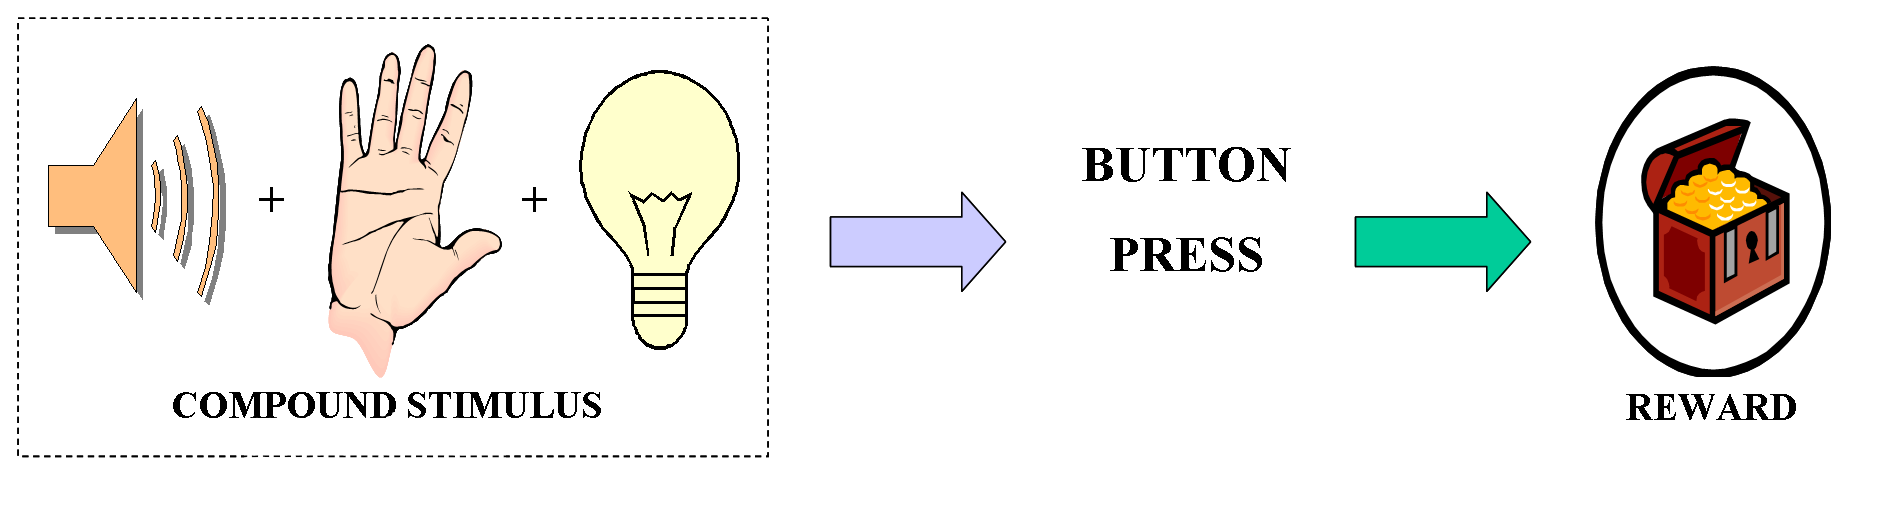
\includegraphics[width=85mm]{figures/compound_stimulus.eps}
%-----------------------------------------------------------
%	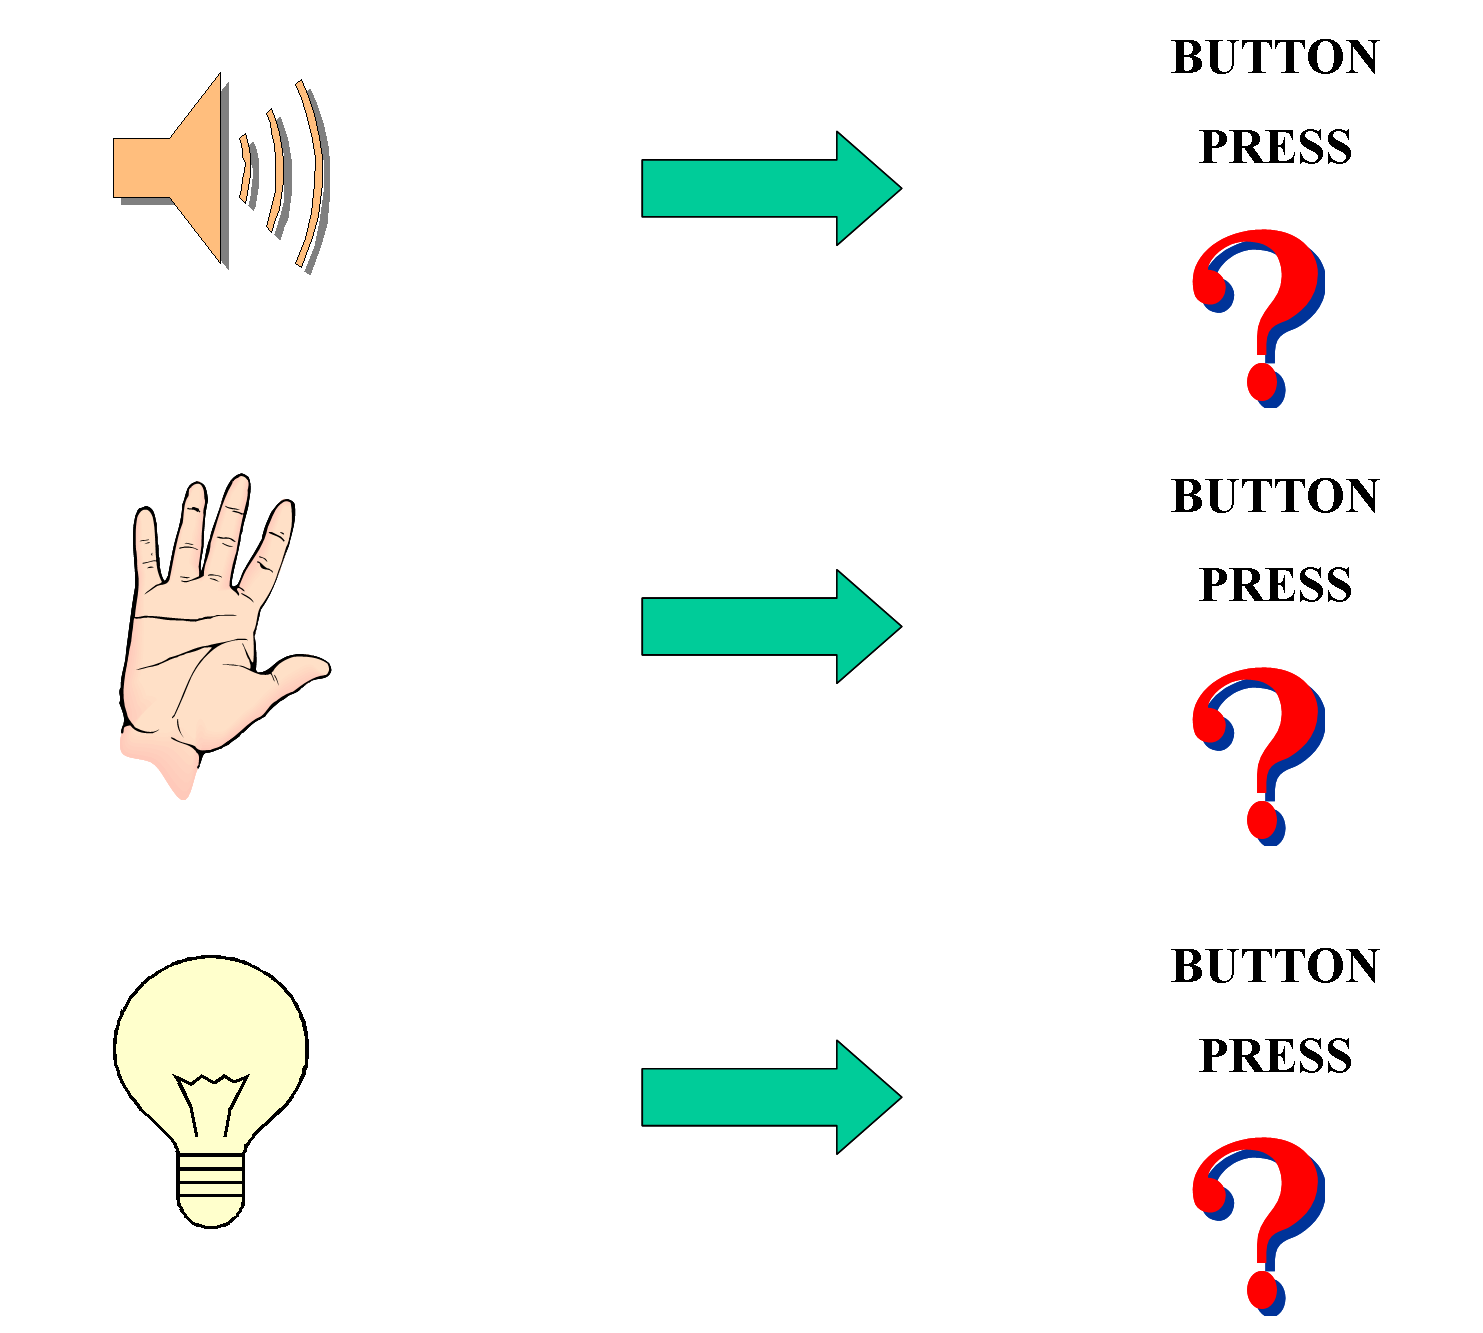
\includegraphics[width=85mm]{figures/components.eps}
%\end{center}
%\caption{Cartoon of task used to assess stimulus overselectivity (Lovaas et al, 1971).  Top panel shows a compound stimulus comprised of an auditory, tactile, and visual stimulus being associated with an action that leads to reward.  The bottom panel represents each component being tested separately in order to assess whether, individually, they have gained sufficient control over behavior to elicit a response.}
%\label{OS-Task}
%\end{figure} 


In the following we propose that deficits in PFC / DA interactions are responsible for many of the interesting behavioral patterns observed in ASD, including executive dysfunction, stimulus overselectivity, and aspects of weak central coherence.  The reduced efficacy of the DA-based gating mechanism on control representations stored within the prefrontal cortex results in overly perseverative attention.  This has two results.  First, the inability to properly adapt the control representations of the PFC produces inflexible behavior.  This behavioral perseveration is manifested in inflexible actions and is exemplified by the executive dysfunction profile in autism.  The second consequence of perturbed DA / PFC interactions is more subtle. We suggest that flexible adjustment of PFC plays an important role in shaping associational areas of cortex in a manner which affords generalization of behavior.  The lack of flexible updating of the PFC results in cortical representations that associate an overly restricted subset of environmental features with appropriate behaviors (e.g. overselectivity).  With only the restricted subset of cues dominating behavior, generalization will be hindered in situations not containing the associated and restricted subset of features.  The resulting learning deficits can be seen in both tests of stimulus overselectivity and in measures of prototype extraction during category learning.  Failure to appropriately update the contents of PFC can also result in an inability to appropriately use temporally extended context information, explaining observed deficits in sequential implicit learning tasks and in the use of sentential context to disambiguate words. 

Next we provide important background information about autism spectrum disorders, a a more detailed description of the interactions between mid-brain dopamine system and the PFC, as well as a brief survey of previous computational modeling efforts seeking to explain behavior of people with autism.  After the relevant background is covered, we summarize using computational modeling techniques how dysfunctional interactions between the DA system and the PFC can account for a wide range of behaviors in people with ASD including Executive Dysfuncion, overselectivity, implicit learning deficits, difficulty with lexical disambiguation, as well as prototype formation.  




\section{Background}
\label{section:background}

% 
% Background
% 

\subsection{Theories of Autism}
Current theories attempting to account for behavior demonstrated by people with autism can coarsely be divided into two categories, psychological and neuroscientific.  Psychological theories attempt to explain behavior in terms of a deficit in a cognitive mechanism, while neuroscientific approaches look towards differences in the anatomy and biology first.  Both approaches have recently begun incorporating information from the other in order to provide a more complete account.  Psychological theories are looking to differences in brain regions which are known to correlate with the specific traits of people with autism.  On the other hand, differences in the neuroanatomy are being matched to behavioral phenomena by identifying similar cognitive deficits in the adult neuropsychological literature, describing how damage to specific brain areas can affect behavior in a developed system.  This unifying approach is encouraging. However, there is still no consensus regarding how to best unify these theories into a testable and coherent framework.  In the following we give a brief overview of the state of theorizing in autism from both the psychological and neuroscientific approaches.
%While the attempt at synergy and general acknowledgment of the need to explain autism in more reductionistic terms is extremely encouraging, there is still no consensus, nor any momentum, towards a particular approach or theory.  The following background is intended to provide context on the current state of theorizing in autism, as well as providing further support and needed details to better support my specific theory of dysfunctional DA / PFC interactions in people with autism.  
	
\subsection{Psychological Approaches}
	Psychological approaches can generally be categorized as either hypothesizing core problems in the social domain or in a more domain general processing mechanism~\cite{RefWorks:85}.  Deficits in the ability to attribute mental states to others, or theory of mind (TOM), has generally been used to explain social difficulties in people with autism~\cite{Baron-Cohen:1985:AutismTOM}.  Under the TOM hypothesis ``Mental states'' refer to things such as our ``beliefs'', ``desires'', and ``intentions''.   In social situations, it is often the case that one needs to infer and interpret another person's ``mental state'' in order to respond in an appropriate manner.  Without this ability, it is suggested one will likely fare poorly in social settings.  The absence of this ability in people with ASD is hypothesized, according to TOM, to be at the core of their social difficulties. 

 While TOM concentrates on social aspects of ASD More domain general processing mechanisms, such as deficits in executive processing or a drive to process information in a ``piecemeal'' manner, are used to explain other aspects of ASD, including perseverative behavior and spared abilities~\cite{HillEL:2004:AutismExecutiveDysfunction}.  The latter piecemeal processing style is the central tennant of the Weak Central Coherence (WCC)~\cite{HappeF:1999:WCC,RefWorks:116} therory.  Under this account strong coherence can be thought of as a tendency to integrate pieces of information into a coherent whole, or global interpretation, of the information. Weak coherence, on the other hand, is the opposite of this tendency~\cite{WitkinHA:1971:EFT}.  In Frith's account of WCC, it is suggested that people with autism exhibit a weak central coherence, processing the world in a local and ``piecemeal'' manner, rather than integrating the local pieces into more coherent and global wholes.  Interestingly, WCC affords the ability to account for the spared, or even enhanced, abilities found in ASD, while still providing an explanation for the differences between normally functioning individuals and those with autism. This is a major strength of WCC.   

The Executive Dysfunction hypothesis views autism as emerging from a deficit in executive control over behavior~\cite{HughesC:1994:AutismExecutiveDysfunction,Ozonoff:1991:AutismExecutiveDysfunction}. This hypothesis is used to account for the rigid, inflexible, and perserverative ``stuck-in-set'' behavior found in autism~\cite{HillEL:2004:AutismExecutiveDysfunction}.  This theory is bolstered by impaired performance on many executive function tasks such as those believed to measure planning (e.g., Tower of Hanoi~\cite{HughesC:1994:AutismExecutiveDysfunction,Ozonoff:1999:AutismStroopWCST}) and cognitive flexibility (e.g., Wisconsin Card Sort Test~\cite{BennettoL:1996:AutismPlanningWCST}).  However, there are unaffected areas of executive functioning found in people with autism, as well.  For instance, cognitive control seems to be relatively unaffected, as measured by the classic Stroop task.  This raises into question the general Executive Dysfunction hypothesis as it has traditionally been cast.  It is possible, however, that the executive problems found in ASD are not necessarily due to damage to the PFC, proper, but arise from problems with other brain structures that have connections with, and affect the functioning of, the frontal lobes~\cite{RobbinsTW:1997:AutismNeurological}.  


%One explanation provided by WCC for the superior performance on the EFT is that the gestalt or holistic view (argued to be the default processing style for normally developing individuals) of the scene could actually hinder or interfere with the search for the individual item. The interference would occur since a global or ``gestalt'' interpretation of the scene would require abstracting information away from the specific parts by definition, thus blurring the distinctions between items, making them less distinguishable.
%This is one example were a ``piecemeal'' processing style is advantageous. Multiple other studies have demonstrated this same pattern.  For example, people with autism have been shown to be less susceptible to certain visual illusions~\cite{RefWorks:125} as well as superior to controls on tasks requiring recreation of a stimulus using blocks containing only pieces of the original~\cite{RefWorks:125}.   On the other hand, people with autism are impaired on tasks requiring the disambiguation of homographs (words with a single spelling but multiple possible meanings and pronunciations such as ``bow'' and ``tear'').  Successfully reading a sentence requires attention to the context of the sentence to succeed.  Studies have found that individuals with autism are less likely than controls to pronounce a homograph correctly when correct pronunciation depends on the context of the sentence~\cite{RefWorks:115}.  In other studies, autistics show the ability to remember individual parts of a sentence, but this comes at the cost of poorer memory for the higher level meaning or ``gist''~\cite{RefWorks:127}.   The results of these studies are consistent with a main tenant of WCC, namely that people with autism lack a robust ability to integrate pieces of information in order to provide more abstract, global, ``gist''-like information.  However, it may be possible to interpret these data in another way --- a way that explains these behaviors in terms of overly perseverative feature based attention.  The problem may not reside in the integration of information, per se.  Instead, the ability to integrate information may still be intact, but all of the features needed for proper integration may not be available to this process.  In other words, abnormal information integration could result from a lack of attention to all parts of the stimulus / situation that are needed to provide the most appropriate abstraction in the current situation.  Overly perseverative attention, a result of perturbed DA / PFC interactions as described earlier, would restrict the feature set that is available, possibly even focusing on idiosyncratic, irrelevant information.  This would result in behavior that looks like a failure to integrate.  Traditionally, the tendency of people with ASD to resist visual illusions is explained in terms of a failure to integrate the pieces (e.g. lines) of the figure, resulting in the lack of a illusory context.  Overly perseverative attention to a restricted set of features may prevent the necessary combination of features to be integrated, preventing the proper context forming to cause the illusory effect.  My conjecture is that, in normally developing individuals, the ability to switch attention across all possible features of the visual stimulus may be required to evoke the illusion.  Similarly, in the EFT, perseverative attention may provide an advantage in this version of a visual search task.  The decreased likelihood of switching the attentional influence of PFC would be an obvious advantage when distracting information could be detrimental to performance.



%Strong coherence can be thought of as a tendency to integrate pieces of information into a coherent whole, or global interpretation, of the information. Weak Central Coherence (WCC)~\cite{HappeF:1999:WCC,RefWorks:116}  can be described as the opposite of this tendency, where the local parts are not gathered into a coherent ``gestalt'', but, instead, are left as atomic elements for processing. In Frith's account of WCC, it is suggested that people with autism exhibit a weak central coherence, processing the world in a local and ``piecemeal'' manner, rather than integrating the local pieces into more coherent and global wholes. It is important to note that this can be seen as a difference in processing styles, rather than a cognitive deficit, per se. This distinction is important because it affords WCC the ability to account for the spared, or even enhanced, abilities found in ASD, while still providing an explanation for the differences between normally functioning individuals and those with autism. This is a major strength of WCC. An example of this unique processing style can be found in the embedded figures test (EFT)~\cite{WitkinHA:1971:EFT}.  

%Generally, science favors reducing explainable phenomena to its most basic components --- to a single explanation if possible.  The current trend in autism research sees this goal as, at best, distant.  The theoretical competition is currently playing out within restricted problem domains in ASD, instead of across domains.  For instance, it is argued by some that we should give up on finding any single mechanism explaining the triad of diagnostic impairments (social, communication, and rigid / perseverative behaviors) in autism~\cite{RefWorks:85}.  Instead, hypotheses are geared towards a subset of behaviors and not viewed as competing with theories attempting to explain behavior outside of their intended scope~\cite{RefWorks:117}.  This is, of course, not always the case, but, does appear to be a general guideline utilized by many theorists. Thus, as the following sections are read, providing a review of the current major psychological theories of autism, it is important to keep in mind that many researchers do \emph{not} see these as competing positions.

%\subsubsection{Theory of Mind}


%In Baron-Cohen's influential 1985 study, a false belief test, known as the ``Sally-Anne'' task, was used to evaluate TOM performance in children with autism, children with Down Syndrome, and a suitable normally developing control group. During the task, two dolls are presented to the child, with one doll (Sally) placing a marble inside of a basket.  Sally then proceeds to leave the area.  While Sally is gone, Anne moves the marble from the basket to a nearby box.  When Sally returns the child is asked, ``Where will Sally look for her marble?''.   

%In this study by Baron-Cohen et al. (1985), 80\% of the children with autism, matched to be of a mental age of at least 4 years old, failed at this task. Importantly, the control groups (on average a \emph{younger} mental age than the autistic group), were easily able to complete the task, realizing that Sally did not see Anne move the marble and will look in the place where it was left.  

%TOM has been one of the most influential and pervasive theories for the past two decades.  However, it seems possible that the success of TOM may lie on intuitive appeal rather than on the ability to provide any precise mechanism (either cognitive or neurobiological) that would be useful to better understand the true nature of the disorder.  For instance, theorists have avoided giving precise reasons for the TOM deficit. Instead, they argue that the TOM problems arise due to problems in a core TOM module.  This module, and its resulting TOM ability, is argued to be innate, even though it is not manifest at birth~\cite{RefWorks:118}.  The claim of innateness is a bold one, and, even if true, would still not explain how this module is implemented.  

%Functional MRI studies have attempted, and often claimed, to have isolated the locus of TOM specific activity in the human brain.  However, a recent article which summarized the findings of the fMRI studies looking at localizing the TOM module~\cite{RefWorks:119} found claims of medial PFC, extrastriate cortex, temporal pole, temporo-parietal junction, cerebellum, thalamus, anterior cingulate, orbital frontal cortex, and precuneus all being implicated as the neural correlate of TOM separately in different studies.  These inconsistent findings must cast some initial doubt on the existence of a TOM module, and subsequently on the possibility that this module is a core deficit in people with ASD.  

%Researchers have also been seeking explanations outside of the realm of TOM to explain performance by people with autism on the false belief tasks.  By controlling some of the executive demands of the task, researchers have found better performance on TOM tasks~\cite{RussellJ:1997:AutismED_TOM,RefWorks:120}.  Very interestingly, Gernsbacher et al. (2005) suggest that deficits found on false belief tasks are actually due to language impairments (which are part of the triad of diagnostic impairments in ASD) and an inability to understand the sentences that are used to explain the tests to children with autism.  In support of this hypothesis, children with specific language impairments, who have no other deficits besides language impairments by definition, fail these false belief tasks~\cite{RefWorks:121}.  In further support of language impairments playing a role in performance of false belief tasks, when a false drawing task is used to assess TOM ability, children with autism \emph{outperform} normally developing children, further calling into question a general TOM deficit in autism~\cite{RefWorks:122}.    


%\subsubsection{Weak Central Coherence}

%TOM deficits are used to provide a possible explanation for a large range of the social deficits found in people with
%autism, but have little to say about other aspects of the cognitive profile in ASD, such as
%attentional abnormalities and problems in generalization.  For instance, children diagnosed with autism tend to focus on parts of play objects, often at the cost of more functional or conventional ways of utilizing the toys~\cite{RefWorks:123,RefWorks:124}.  It is unclear how a deficit in attributing mental states would lead to such a pattern of behavior.  Other theories, such as Weak Central Coherence (WCC), are focused on explaining such attentional abnormalities demonstrated by people with autism. 
%
%Strong coherence can be thought of as a tendency to integrate pieces of information into a coherent whole, or global interpretation, of the information. Weak Central Coherence (WCC)~\cite{HappeF:1999:WCC,RefWorks:116}  can be described as the opposite of this tendency, where the local parts are not gathered into a coherent ``gestalt'', but, instead, are left as atomic elements for processing. In Frith's account of WCC, it is suggested that people with autism exhibit a weak central coherence, processing the world in a local and ``piecemeal'' manner, rather than integrating the local pieces into more coherent and global wholes. It is important to note that this can be seen as a difference in processing styles, rather than a cognitive deficit, per se. This distinction is important because it affords WCC the ability to account for the spared, or even enhanced, abilities found in ASD, while still providing an explanation for the differences between normally functioning individuals and those with autism. This is a major strength of WCC. An example of this unique processing style can be found in the embedded figures test (EFT)~\cite{WitkinHA:1971:EFT}.  
%
%The task involves finding a simple image (e.g., a triangle), embedded within a much more complex scene (e.g., a drawing of a baby carriage). Performance of people with autism on this task has been shown to be superior to that of controls~\cite{RefWorks:104,RefWorks:103}. 


%One explanation provided by WCC for the superior performance on the EFT is that the gestalt or holistic view (argued to be the default processing style for normally developing individuals) of the scene could actually hinder or interfere with the search for the individual item. The interference would occur since a global or ``gestalt'' interpretation of the scene would require abstracting information away from the specific parts by definition, thus blurring the distinctions between items, making them less distinguishable.
%This is one example were a ``piecemeal'' processing style is advantageous. Multiple other studies have demonstrated this same pattern.  For example, people with autism have been shown to be less susceptible to certain visual illusions~\cite{RefWorks:125} as well as superior to controls on tasks requiring recreation of a stimulus using blocks containing only pieces of the original~\cite{RefWorks:125}.   On the other hand, people with autism are impaired on tasks requiring the disambiguation of homographs (words with a single spelling but multiple possible meanings and pronunciations such as ``bow'' and ``tear'').  Successfully reading a sentence requires attention to the context of the sentence to succeed.  Studies have found that individuals with autism are less likely than controls to pronounce a homograph correctly when correct pronunciation depends on the context of the sentence~\cite{RefWorks:115}.  In other studies, autistics show the ability to remember individual parts of a sentence, but this comes at the cost of poorer memory for the higher level meaning or ``gist''~\cite{RefWorks:127}.   The results of these studies are consistent with a main tenant of WCC, namely that people with autism lack a robust ability to integrate pieces of information in order to provide more abstract, global, ``gist''-like information.  However, it may be possible to interpret these data in another way --- a way that explains these behaviors in terms of overly perseverative feature based attention.  The problem may not reside in the integration of information, per se.  Instead, the ability to integrate information may still be intact, but all of the features needed for proper integration may not be available to this process.  In other words, abnormal information integration could result from a lack of attention to all parts of the stimulus / situation that are needed to provide the most appropriate abstraction in the current situation.  Overly perseverative attention, a result of perturbed DA / PFC interactions as described earlier, would restrict the feature set that is available, possibly even focusing on idiosyncratic, irrelevant information.  This would result in behavior that looks like a failure to integrate.  Traditionally, the tendency of people with ASD to resist visual illusions is explained in terms of a failure to integrate the pieces (e.g. lines) of the figure, resulting in the lack of a illusory context.  Overly perseverative attention to a restricted set of features may prevent the necessary combination of features to be integrated, preventing the proper context forming to cause the illusory effect.  My conjecture is that, in normally developing individuals, the ability to switch attention across all possible features of the visual stimulus may be required to evoke the illusion.  Similarly, in the EFT, perseverative attention may provide an advantage in this version of a visual search task.  The decreased likelihood of switching the attentional influence of PFC would be an obvious advantage when distracting information could be detrimental to performance.

%\subsubsection{Executive Dysfunction}
%The Executive Dysfunction hypothesis views autism as emerging from a deficit in executive control over behavior~\cite{HughesC:1994:AutismExecutiveDysfunction,Ozonoff:1991:AutismExecutiveDysfunction}. This hypothesis is used to account for the rigid, inflexible, and perserverative ``stuck-in-set'' behavior found in autism~\cite{HillEL:2004:AutismExecutiveDysfunction}.  Executive functioning is used as an umbrella term for a variety of deliberate and modulatory processes, such as planning, cognitive control, and cognitive flexibility.  These processes are traditionally associated with frontal neural circuits, evidenced by deficits in tasks thought to measure executive processing in frontally damaged patients~\cite{Stuss:2000:WCSTLesion,Stuss:2001:StroopLesion}.  This theory is bolstered by impaired performance on many executive function tasks such as those believed to measure planning (e.g., Tower of Hanoi~\cite{HughesC:1994:AutismExecutiveDysfunction,Ozonoff:1999:AutismStroopWCST}) and cognitive flexibility (e.g., Wisconsin Card Sort Test~\cite{BennettoL:1996:AutismPlanningWCST}).  However, there are unaffected areas of executive functioning found in people with autism, as well.  For instance, cognitive control seems to be relatively unaffected, as measured by the classic Stroop task.  This raises into question the general Executive Dysfunction hypothesis as it has traditionally been cast.  It is possible, however, that the executive problems found in ASD are not necessarily due to damage to the PFC, proper, but arise from problems with other brain structures that have connections with, and affect the functioning of, the frontal lobes~\cite{RobbinsTW:1997:AutismNeurological}.  It is just these kinds of questions ---whether executive problems can be explained in terms of the dysfunction of specific neural circuits interacting with PFC--- which computational models are well suited to help us explore.
%

%\subsubsection{Stimulus Overselectivity}
%Since Kanner's original description of ``early infantile autism'' in 1943, it has been noted that people with autism seem to be preoccupied with specific and sometimes peculiar parts of objects and situations~\cite{KannerL:1943:Autism}. In 1971 this phenomena was operationalized and termed ``stimulus overselectivity''.  In the seminal study in this paradigm, a compound stimulus comprised of auditory, visual, and tactile components was presented to both low functioning children with autism and age matched control subjects. (See Figure~\ref{OS-Task}.)  Initially, the subjects were trained to respond to the compound stimulus via an operant conditioning paradigm.  Participants were rewarded when they made a specific action (e.g. lever press) when the compound stimulus was presented.  After the acquisition of this initial stimulus / response pairing, each individual component was presented separately to assess the degree to which the individual components, themselves, had acquired control of the behavior.  In the normally functioning control group, the participants responded equally to each of the individual components of the stimulus, demonstrating a lack of overselectivity.  The group consisting of people with autism, however, responded to only one component of the three tested, thus demonstrating overselectivity.  No systematic preference between the components was noted across subjects.   This important result demonstrated how behavior in people with autism may be dominated by a small, restricted feature set, as compared to what is actually available in the environment.  This result has been replicated across various modalities~\cite{RefWorks:128,RefWorks:129} and even when varying the number of features~\cite{RefWorks:131}.  

%A major implication of overselectivity is a reduced ability to generalize learned behaviors and general associations to novel settings.  A study investigating why people with autism fail to generalize a newly learned behavior to a novel setting initially had each individual with autism taught a new behavior (e.g. to raise their right arm when the phrase, ``raise your right arm'' was spoken).  After the initial behavior acquisition phase, the individuals were moved to a new location, which included a new experimenter, and tested the ability to generalize and perform the recently learned behavior in the novel setting.  Next, for those participants who failed the generalization phase, items from the original setting were systematically introduced in order to determine exactly what had been learned by the participants with autism.  Each of the participants who had failed to generalize appeared to be reliant on very specific, often idiosyncratic, pieces of the original training situation where the behavior was initially learned.  For instance, one individual required the exact same hand movements, made by the original experimenter, to be made by the new experimenter in the new situation for any transfer to occur.  Another person with autism needed the table and chairs from the original room to be present before he would transfer the learned behavior to the novel environment.  Generalization is problematic in people with autism, based on these and similar reports, due to learning associations between the desired behavior and a restricted, possibly irrelevant, set of information. Failure to generalize learned behaviors is a major concern for many, if not all, intervention techniques used in autism treatment.  Indeed, reducing overselectivity is a key ingredient in many of the most used therapies for children with autism~\cite{RefWorks:130,RefWorks:132}.


%My theory of dopamine / PFC mediated perseverative attention in people with autism suggests that overselectivity is a result of the inability to appropriately switch the sustained modulatory influences of PFC on other cortical areas.  Initial modeling results demonstrate that switching of PFC representations between different aspects of the stimulus results in performance matching normal control subjects.  Namely, each individual component is able to elicit a response separate from others, showing no overselectivity.  However, not allowing the PFC to flexibly update its control state, as we argue is the case in people with autism, results in overselective responding to a restricted number of the possible features. (See Chapter 4.)  It is worth noting that this result could have important implications, providing a possible cognitive and neural mechanism explaining how people with autism come to develop overselective responding to parts of their environment.


\subsection{Neurobiology}

Autistic deficits are widely believed to have a neurological origin.  However, neuroscientific frameworks to date have had little success in providing a unifying view of the neural mechanisms responsible for behavior in autism.   Indeed, the vast amount of variance in brain regions implicated as possible underlying neural substrates in ASD makes the task of identifying a unified neuroscientific account somewhat daunting. Caveats aside, there are many neurobiological differences thought to exist in ASD that are worth further exploration. In the end, all consistent underlying differences in the neurobiology need to be accounted for by any complete theory, or combination of theories, seeking to explain autism. 

One of the most consistent neuroimaging findings in people with ASD is abnormalities of structure within the cerebellum~\cite{AkshoomoffNA:2000:Neurological,RefWorks:133}. These findings consist of hypoplasia (reduced growth) and hyperplasia (increased growth)~\cite{RodierPM:1996:AutismCerebellum} within the cerebellar vermis. Dysfunction of the cerebellum may account for some of the motor difficulties found in people with autism, since the cerebellum is known to be important for coordinated motor control.  Interestingly, some researchers are also actively pursuing the possible role the cerebellum may play in shifting our attention~\cite{RefWorks:135,CourchesneE:1994:CerebellumAttentionShift}.  Studies investigating this possibility have shown that people with autism and patients with cerebellar lesions perform similarly on tasks requiring the ability to rapidly shift attention between different dimensions of sets of stimuli~\cite{CourchesneE:1994:CerebellumAttentionShift,RefWorks:136,RefWorks:134}.  This view of the potential behavioral consequence of cerebellar abnormalities is similar to the perseverative attention account we are suggesting.  However, since the underlying mechanism is different, it is possible to distinguish between the two theories experimentally.  For instance, a study comparing differences in patients with cerebellar dysfunction to those with Parkinson's disease, a disorder of the mid-brain dopamine system, shows that behavior is indeed different on tasks requiring shifts of attention~\cite{RefWorks:145}.  While both patient populations performed worse than control groups, only the group with cerebellar pathology showed improvement when the motor demands of the task were reduced.  This suggests that the deficits in switching attention due to cerebellar abnormalities may be due, at least in part, to motoric demands of the task. 

A theory which has recently caught the attention of the scientific community and the general population alike suggests that TOM and ``mind reading'' deficits in people with autism may result from problems in the ``mirror neuron'' system.  Mirror neurons, initially discovered in the F5 area of premotor cortex in non-human primates,  fire selectively when the animal performs specific goal directed actions~\cite{RefWorks:140}.  Interestingly, these same cells would also respond to the monkey watching another monkey or human performing the same action.  The discovery of cells which appear to respond symmetrically to a performed and observed action have led some researchers to suggest that the mirror neuron system could be vital for imitation skills and even TOM abilities in humans, and damaged mirror systems could therefore help explain the social deficits found in people with autism~\cite{RefWorks:141,RefWorks:138}.     

Structural MRI analysis investigating overall brain volume in people with ASD have discovered increased cerebral (white matter) volumes in people with ASD~\cite{FilipekPA:1995:AutismCerebellumMRI}, which are argued to be due to a failure in cortical pruning which occurs early in development~\cite{Eigsti:2003:AutismNeuroReview}.  One study investigating the time course of brain growth in children with autism indicates that children with autism have larger brains than normal early in development (12 years and younger), but, by adolescence, have returned to normal compared with age matched controls~\cite{RefWorks:142}.  It is not immediately clear what effect the overgrowth of neural connections would have on behavior, but some theories suggest that possible effects might include the rigid and context specific patterns of behavior seen in ASD~\cite{CohenIL:1994:AutismLearning}.

The limbic system is of interest in autism research largely due to its suggested role in social and emotional behavior, both believed to be problematic in autism.  Postmortem anatomical studies were able to find consistent abnormalities only in the limbic system of the autistic brains analyzed~\cite{RefWorks:133}, supporting a possibly unique role for the limbic system in autism. Also, controlled damage to the amygdala has provided an interesting animal model of autism~\cite{BachevalierJ:1994:AutismAnimalModel}.  Other areas of the limbic system, including the hippocampus, anterior cingulate gyrus, and hypothalamus have been investigated and implicated as possible sites for the neural substrate of ASD~\cite{RefWorks:133}.  

Inspired partially by links to executive function deficits in ASD and partly by neuroanatomical findings, the PFC is an area of key interest for many ASD researchers. Anatomically, researchers have identified the possibility of ``narrow mini-columns'' in the PFC~\cite{Casanova:2003:AutismMiniColumns} and have noted that the parietal, temporal, and occipital lobes show overall brain volume enlargements, while the frontal lobes show no such increase. The lack of an increase means that the frontal lobes may be considered smaller in volume when compared with the relative scaling of the rest of the brain~\cite{PivenJ:1996:AutismBrainBig}. Considering the many executive functioning problems observed in ASD, the PFC stands out as, at a minimum, a likely indirect player in some of the unusual behavior displayed in autism.

Lastly, neurotransmitter systems are of particular interest in the search for the brain basis of autistic behavior since, due to their diffuse global nature, there is potential for the neurochemicals to affect multiple brain regions. Using techniques as diverse as urinalysis and PET imaging, differential amounts of serotonin and dopamine (DA) have been identified in people with autism~\cite{FernellE:1997:AutismPET,MartineauJ:1992:AutismDopamine,PoseyDJ:2000:AutismDopamine,RefWorks:72} compared to controls, while clinical trials investigating the efficacy of drugs affecting levels of dopamine and serotonin in the brain have had mixed results~\cite{MartineauJ:1992:AutismDopamine,PoseyDJ:2000:AutismDopamine,Chugani:2004:AutismSerotonin}.  While serotonin and dopamine appear to be the most active areas of investigation for neurochemical abnormalities in ASD, other differences in brain chemistry have been observed.  Glutamatergic, GABA, and cholinergic abnormalities have been identified~\cite{RefWorks:95,RefWorks:96,RefWorks:137}.  Also oxytoxin and vasopression have been investigated as a possible source of problematic behavior in people with ASD~\cite{RefWorks:95,RefWorks:75}.

%\subsubsection{Prefrontal Cortex (PFC)}
%Inspired partially by links to executive function deficits in ASD and partly by neuroanatomical findings, the PFC is an area of key interest for many ASD researchers. Anatomically, researchers have identified the possibility of ``narrow mini-columns'' in the PFC~\cite{Casanova:2003:AutismMiniColumns} and have noted that the parietal, temporal, and occipital lobes show overall brain volume enlargements, while the frontal lobes show no such increase. The lack of an increase means that the frontal lobes may be considered smaller in volume when compared with the relative scaling of the rest of the brain~\cite{PivenJ:1996:AutismBrainBig}. Considering the many executive functioning problems observed in ASD, the PFC stands out as, at a minimum, a likely indirect player in some of the unusual behavior displayed in autism.


%Proponents of a cerebellar role in switching attention suggest that the cerebellum provides a modulatory signal to appropriate areas of the brain, preparing these areas for upcoming use in a task appropriate manner~\cite{RefWorks:134}.  Damage to this mechanism leads to perseverative and inflexible behavior.  Recent studies have cast some doubt as to whether the tasks used are truly unmasking a deficit in attention shifting, however~\cite{RefWorks:143,RefWorks:144}.  It is worth noting that there are similarities between the cerebellar dysfunction theory of autism and the theory presented in this thesis, which includes a deficient dopamine based gating mechanism in PFC.  Both theories make similar cognitive predictions, suggesting that a core problem in people with autism lies in their inability to switch attention appropriately.  However, since the underlying mechanism is different, deficits in each system still can make unique predictions differentiating the theories.  For instance, a study comparing differences in patients with cerebellar dysfunction to those with Parkinson's disease, a disorder of the mid-brain dopamine system, shows that behavior is indeed different on tasks requiring shifts of attention~\cite{RefWorks:145}.  While both patient populations performed worse than control groups, only the group with cerebellar pathology showed improvement when the motor demands of the task were reduced.  This suggests that the deficits in switching attention due to cerebellar abnormalities may be due, at least in part, to motoric demands of the task. 

%Researchers are also actively pursuing the possibility of cerebellar influence on
%attention and attention shifting (Courchesne, 1987), which might help explain attentional
%differences found in autism.

%ADD DOPAMINE LINKS TO FOLLOWING SECTIONS?

%\subsubsection{Mirror Neurons}
%A theory which has recently caught the attention of the scientific community and the general population alike suggests that TOM and ``mind reading'' deficits in people with autism may result from problems in the ``mirror neuron'' system.  Mirror neurons, initially discovered in the F5 area of premotor cortex in non-human primates,  fire selectively when the animal performs specific goal directed actions~\cite{RefWorks:140}.  For instance, movement of the monkey's hand with the goal of placing a piece of food in the monkey's mouth would elicit firing of a specific set of mirror neurons.  Interestingly, these same cells would also respond to the monkey watching another monkey or human performing the same action.  The discovery of cells which appear to respond symmetrically to a performed and observed action have led some researchers to suggest that the mirror neuron system could be vital for imitation skills and even TOM abilities in humans~\cite{RefWorks:141}.  Subsequently, autism researchers have suggested that perhaps the social and ``mind reading'' problems demonstrated by people with ASD could be, at least in part, due to an inadequate or damaged mirror neuron system~\cite{RefWorks:138}.       

%\subsubsection{Brain Volume and Structure}
%Structural MRI analysis investigating overall brain volume in people with ASD have discovered increased cerebral (white matter) volumes in people with ASD~\cite{FilipekPA:1995:AutismCerebellumMRI}, which are argued to be due to a failure in cortical pruning which occurs early in development~\cite{Eigsti:2003:AutismNeuroReview}.  One study investigating the time course of brain growth in children with autism indicates that children with autism have larger brains than normal early in development (12 years and younger), but, by adolescence, have returned to normal compared with age matched controls~\cite{RefWorks:142}.  It is not immediately clear what effect the overgrowth of neural connections would have on behavior, but some theories suggest that possible effects might include the rigid and context specific patterns of behavior seen in ASD~\cite{CohenIL:1994:AutismLearning}.

%DA is known to have effects on neurogenesis...

%\subsubsection{Limbic System}
%The limbic system is of interest in autism research largely due to its suggested role in social and emotional behavior, both believed to be problematic in autism.  Postmortem anatomical studies were able to find consistent abnormalities only in the limbic system of the autistic brains analyzed~\cite{RefWorks:133}, supporting a possibly unique role for the limbic system in autism. Also, controlled damage to the amygdala has provided an interesting animal model of autism~\cite{BachevalierJ:1994:AutismAnimalModel}. In this animal model, selective ablation of the amygdala was performed in rhesus monkey subjects. The lesioned monkeys displayed repetitive motor behaviors, as well as ``autistic-like'' social behaviors such as active social avoidance and lack of eye contact.  Other areas of the limbic system, including the hippocampus, anterior cingulate gyrus, and hypothalamus have been investigated and implicated as possible sites for the neural substrate of ASD~\cite{RefWorks:133}.  

%\subsubsection{Prefrontal Cortex (PFC)}
%Inspired partially by links to executive function deficits in ASD and partly by neuroanatomical findings, the PFC is an area of key interest for many ASD researchers. Anatomically, researchers have identified the possibility of ``narrow mini-columns'' in the PFC~\cite{Casanova:2003:AutismMiniColumns} and have noted that the parietal, temporal, and occipital lobes show overall brain volume enlargements, while the frontal lobes show no such increase. The lack of an increase means that the frontal lobes may be considered smaller in volume when compared with the relative scaling of the rest of the brain~\cite{PivenJ:1996:AutismBrainBig}. Considering the many executive functioning problems observed in ASD, the PFC stands out as, at a minimum, a likely indirect player in some of the unusual behavior displayed in autism.


%\subsubsection{Neurotransmitters}
%Neurotransmitter systems are of particular interest in the search for the brain basis of autistic behavior since, due to their diffuse global nature, there is potential for the neurochemicals to affect multiple brain regions. This fact is compelling given the heterogeneity found in both the functional and anatomical properties discovered thus far in the neural systems of people with ASD.

%Using techniques as diverse as urinalysis and PET imaging, differential amounts of serotonin and dopamine (DA) have been identified in people with autism~\cite{FernellE:1997:AutismPET,MartineauJ:1992:AutismDopamine,PoseyDJ:2000:AutismDopamine,RefWorks:72} compared to controls.  Clinical trials investigating the efficacy of drugs affecting levels of dopamine and serotonin in the brain have had mixed results~\cite{MartineauJ:1992:AutismDopamine,PoseyDJ:2000:AutismDopamine,Chugani:2004:AutismSerotonin}. Many drugs showed a benefit in reducing some problematic behaviors in autism, such as disruptiveness and self injurious behavior, while exasperating others, such as stereotypical and repetitive behavior.  To date, there has been no investigation concerning the effect of anti-psychotics on controlled tasks of cognitive performance, such as the Wisconsin Card Sort Task.  Such investigations could provide extremely useful insights into how specific neurochemicals are affecting behavior in autism.

%While serotonin and dopamine appear to be the most active areas of investigation for neurochemical abnormalities in ASD, other differences in brain chemistry have been observed.  Glutamatergic, GABA, and cholinergic abnormalities have been identified~\cite{RefWorks:95,RefWorks:96,RefWorks:137}.  Also oxytoxin and vasopression have been investigated as a possible source of problematic behavior in people with ASD~\cite{RefWorks:95,RefWorks:75}.


\subsection{Previous Computational Models of Autism}

The formal and explicit nature of computational cognitive modeling suggests a novel approach to autism research.  In order for computational models to be useful in this endeavor, they must be constrained by both bottom-up (neurobiological mechanisms) and by top-down (observed behavior) considerations.  It is not at all clear that the current computational models attempting to provide explanations for the behavior of people with autism have accomplished these goals.  Previous computational models have been published attempting to address various behavioral aspects of autism including poor generalizing~\cite{CohenIL:1994:AutismLearning,GustafssonL:1997:AutismMaps}, Weak Central Coherence~\cite{OLoughlinC:2000:Coherence}, overselectivity~\cite{McClellandJL:2000:Autism}, as well as Grossberg \& Seidman (2006)~\nocite{RefWorks:146} ambitious computational framework seeking to explain multiple aspects of autism including poor generalization as well as cognitive and emotional issues.

A short coming of many of the existing models of autism is their fairly abstract in nature, making little contact with specific neurobiological considerations~\cite{CohenIL:1994:AutismLearning,McClellandJL:2000:Autism,OLoughlinC:2000:Coherence}.  Even those models of autism which have incorporated biology into their framework have thus far only matched qualitative patterns of behavior in people with ASD, not attempting to account for any quantitative behavioral data~\cite{GustafssonL:1997:AutismMaps,RefWorks:146}.  Models more tightly coupled with observed functional properties of neurobiological systems and constrained by actual behavioral data will be able to more precisely inform theories of ASD. 


%\subsection{The Problem with Overfitting}

%Cohen was the first researcher to report on a neural network model designed to explain patterns of behavior in people with ASD~\cite{CohenIL:1994:AutismLearning}.  Cohen's model rests on the notion that neural networks, when allowed to have too many units in a hidden layer, are likely to fall prey to the problem of ``overfitting'' the training data.  When training a neural network, one wishes to capture the true functional form (or at least the best possible approximation) of the task, as implicitly characterized by the training data.  By capturing the form of the function, the model is able to generalize to inputs that it has not been exposed to in the past.  When ``overfitting'' occurs, instead of capturing the true underlying functional form, the model essentially memorizes the specific training data items.  This results in precisely correct performance when the network experiences the training situations again, but poor performance on novel inputs.  In other words, overfitting results in poor generalization.  

%Cohen cites studies that have found that many areas of the brain, with a particular focus on the amygdala and hippocampus, exhibit an overall increase in the number of neurons in people with autism as compared to controls, Cohen argues that an analog between overfitting in neural networks and poor generalization, as seen in people with ASD, can be made.  Cohen conjectures that since the amygdala is implicated in emotional and social processing, too many neurons could result in a kind of ``overfitting'' of socially relevant stimuli, resulting in unrelated and unimportant features of a social situation being taken into account when learning appropriate social behavior.  The unrelated information will usually only hinder the ability to act appropriately in the extremely subtle and complex acts of social interactions, explaining the overall poor social abilities and lack of ability to generalize to new situations found in people with ASD.  A computational model is provided which demonstrates that, as the number of hidden layer units increase, the ability of the network to generalize to new inputs deteriorates.  Furthermore, it is argued that the savant-like abilities found in some people with autism can be explained as an overall increase in the number of neurons which are employed in the task.  For instance, Cohen suggests that if a person with autism has an extraordinary ability in a specific modality then, according to his theory, we should find an increased number of neurons in the network facilitating the learning of that modality (e.g., visual) and not in areas used for other modalities (e.g., haptic or auditory).

%Cohen's hypothesis of ``too many'' neurons resulting in a type of behavioral ``overfitting'' has some intuitive appeal, especially when analyzing how neural networks perform as a function of the number of processing units.  However, the model does not possess any solid fits to any specific quantitative behavioral data.  Instead it relies on a more abstract, verbally justified, account of how poor generalization arises in people with ASD.  Also, links to underlying neurobiological systems are of an almost anecdotal nature, casually noting that some postmortem studies have found an increased number of neurons in some areas of the brain in people with autism.

%\subsection{Inadequate Cortical Feature Maps}
%Gustafsson's modeling of inadequate cortical feature maps in autism follows in the footsteps of Cohen's attempt to explain good discrimination skills and poor generalization skills found in people with ASD~\cite{GustafssonL:1997:AutismMaps}.  In this endeavor, Gustafsson argues that overly narrow neural columns in people with autism are at the core of this pattern of behavior.  Cortex is believed to be organized in a columnar manner, with the neurons in each column possessing similar receptive field properties.  Neurons within a column in cortex tend to respond to the same aspects of a stimulus, resulting in a type of ``cortical feature map''.  If these neural columns are overly narrow, then, as Gustafsson writes, ``feature detection will only be possible if the set of features very closely corresponds to that which the neural column has become identified with, i.e., there must not be much variability in features'', and he follows, ``an individual with such an inadequate feature map must insist on precision or `sameness' ''.  This desire for ``sameness'' is a common behavioral feature found in people with ASD.  The thrust of the inadequate feature map hypothesis is that narrower neural columns in cortex will have narrower receptive field properties (responsive to a smaller than normal range of stimuli) and therefore exhibit good discrimination but poor generalization.

%The artificial neural network discussed in Gustafsson's 1997 article is based on networks developed by Kohonen~\cite{kohonen84selforg}, which include excitatory and inhibitory lateral feedback connections in a neighborhood-like structure.  This means that units within a certain distance of each other will contain mutually excitatory connections, while outside of this distance the connections to other units will be inhibitory~\cite{vod_der_MalsburgC:1973:SOM_Striate}.  This relationship causes a topological structure to develop in the models, with columnar-like groupings of units which respond in a similar manner to stimulus features.  An important property of these networks is that the Kohonen map learns its fundamental properties through extensive exposure to stimuli.  No set structure for stimulus representation is assumed to exist a priori.  This property allows for the possibility that inadequate feature maps will arise somewhat naturally during development, simply by manipulating a single parameter, namely increasing the level of lateral inhibition, in the model.  Gustafsson proceeds to provide a mathematical proof, based on previous findings~\cite{kohonen84selforg}, that as you increase the overall lateral inhibition, the columns in the Kohonen maps become narrower and respond to a smaller set of stimulus features.  In other words, they develop smaller receptive fields.

%Unlike the previous models, Gustafsson's model makes strong contact with underlying biological mechanisms.  However, considering the high comorbidity of seizures in the disorder it is unclear whether excessive lateral inhibition is justified~\cite{Casanova:2003:AutismMiniColumns}.  It is difficult to analyze the performance of the model, as no actual model simulation results were presented.  Therefore, the same critique of Cohen's work holds for Gustafsson's model: there is no evidence that the model will be able to provide a tight quantitative fit to actual behavioral data.   

%\subsection{Weak Central Coherence as Constraint Satisfaction}

%O'Loughlin and Thagard provide a computational modeling account of Frith's theory of weak central coherence~\cite{FrithU:1989:AutismWCC} by simulating coherence using a constraint satisfaction network~\cite{OLoughlinC:2000:Coherence}.  A constraint satisfaction problem can be roughly described as follows: Given a set of possible states of the world, of which some states may be less likely to coincide simultaneously with  others (e.g., it is not likely to be outside while it is raining, and not get wet), what set of states maximally satisfy all possible constraints?  A constraint satisfaction network embodies a constraint satisfaction problem where the different aspects of possible states of the world are specified as nodes in the network, and the constraints between these states are embodied by numeric weights on the connections between these nodes.  For an exclusivity constraint between two different states (representing the concept that the two states are not likely to occur together, e.g., eating and being asleep at the same time), a negative weight value is used, and for a co-occurrence constraint (representing when the two states are likely to occur together, e.g., being thirsty and drinking water) a positive weight value is used.  ``Normal'' coherence is taken to be the network functioning in the standard manner, maximally choosing the states which satisfy the most constraints.  WCC is simulated as pushing the network to settle upon a sub-optimal set of states, which do not maximally satisfy all of the constraints. 

%To make this more clear, it is helpful to consider the simulation provided by O'Loughlin and Thagard using the Sally-Anne task~\cite{Baron-Cohen:1985:AutismTOM}.  To simulate this task, the nodes of the network are coded to represent possible states in the task such as ``Sally puts marble in basket'' and ``Anne transfers marble to box while Sally is away'', with positive connections (positive constraint) between the states and negative connections (negative constraints) between nodes such as ``Sally looks in basket'' and ''Sally looks in box''.  The different states and constraints between them represent a kind of ``knowledge network'' of the Sally-Anne task.  If the constraints are set up properly, the network will settle on the correct hypothesis, that ``Sally looks in basket''.  

%In order to simulate WCC as seen in children with autism, the negative constraints (connections) were increased, making the inhibitory connections stronger than the excitatory connections.  This manipulation results in the network settling prematurely and most likely in a state that did not satisfy all of the original constraints in the network.  In the simulation of the Sally-Anne task, the solution resulting in the incorrect choice of ``Sally looks in box'' is essentially ``shorter'' and simpler than the correct, but unfortunately more causally complex, choice ``Sally looks in basket''.  This allows the increased inhibition to result in the network guessing incorrectly, ``Sally looks in box'', since when the network has finished the settling process, it will satisfy the most modified constraints in the constraint satisfaction network.

%The modeling approach used is extremely abstract in nature, with all of the knowledge of how the problem is to be solved pre-specified within the structure of the network (i.e., the nodes and the constraints between them).  It is unclear whether the mechanism employed to simulate performance of people with autism on the Sally-Anne task, namely increased inhibition in the network, can be biologically supported, considering, once again, the high comorbidity of seizures in the disorder~\cite{Casanova:2003:AutismMiniColumns} as well as lack of any other justification from the authors.  While the model is used to capture qualitative behavioral performance on the Sally-Anne task (as well as an example of a homograph task using the same approach), it is unclear how the model would fare at capturing quantitative behavioral data on these tasks.


%\subsection{Hyperspecificity}
%McClelland takes a slightly different approach to the same issues of poor generalization and stimulus overselectivity (or hyperspecificity) addressed by the models previously mentioned~\cite{McClellandJL:2000:Autism}.  Instead of providing a model, or even a description of a model, McClelland provides a general description of some of the properties of neural networks which could give rise to hyperspecificity at the cost of the ability to generalize.  Conjunctive codes in neural networks are representations that consist of components that, instead of responding to individual features of input (e.g., either ``red'' or ``square''), only respond to conjunctions of the input features (e.g., ``red square'').  As the number of conjuncted features required to activate a processing unit increases, the network's representation of the current situation becomes more specific (e.g., only responding to small green circles with radial lines, etc.).  Conjunctive representations are useful when the stimulus is actually a conjunction of features (e.g., a chair is a conjunction of many smaller components such as the seat, legs, back, etc.), however, this coding scheme can hinder generalization, since each unit only responds to a specific conjunction of features.  McClelland introduces the possibility that children with autism posses overly conjunctive representations of the environment.  This could account for hyperspecificity found in people with ASD.  McClelland provides an anecdotal story of a child with autism who refuses to use the restroom at a friends house because it is unfamiliar.  In other words, it is not the specific bathroom with which he is familiar.  If we think of the bathroom which the child with autism uses at his home, it may posses items such as green walls, a toilet, tile on the floor, etc., none of which are present in the friends home, with the likely exception of the toilet.  Perhaps, McClelland argues, the child represents the toilet with an overly conjunctive representation that includes other contextual items such as the color of the walls, the tile on the floor, etc.  

%Perhaps the largest problem with McClelland's modeling theory of hyperspecificity in autism is that no computational model ---not even a precise \emph{description} of a model--- is provided.  Many details would need to be specified before such a general verbal description could be brought in contact with quantitative behavioral data.  Also, the theory does not address what neurobiological differences in people with autism might give rise the overly conjunctive code argued to provide a possible account of hyperspecificity in ASD\footnote{McClelland is no longer a proponent of the overly-conjunctive hypothesis described here (Personal Communication, 2007).}.

%\subsection{iSTART}
%Grossberg \& Seidman (2006)~\nocite{RefWorks:146} provide a recent, ambitious, and complex computational model seeking to explain behavior in people with autism to date, known as iSTART (Imbalanced Spectraly Timed Adapative Resonance Theory).  The iSTART model of autistic performance stands on the shoulders of three previous modeling frameworks, ART --- ``Adaptive Resonance Theory'', CogEM --- ``Cognitive - Emotional - Motor'', and the ``Spectral Timing'' model.  ART proposes how the brain learns to categorize objects and events.  According to ART, when an object is experienced in the environment, perceptually driven bottom-up representations are compared with previously learned top-down expectations. If there is sufficient overlap or similarity between top-down and bottom-up representations, then a ``recognition process'' is instantiated.  However, if there is not sufficient similarity, then the object is determined to be novel, and a different process is instantiated to add the object as a new category.  The amount of similarity that is required to determine whether an object is novel or not is determined by a single parameter termed ``vigilance''.  It is proposed that people with autism are hyper-vigilant, resulting in overly specific category structures.  The hyper-specific category structures are argued to be at the root of the overly specific kinds of processing demonstrated by people with autism and traditionally accounted for by theories such as weak central coherence.  

%It is unclear how the vigilance manipulation would be able to account for the overselective behavior seen in people with autism.  Rather, the prediction of the model seems to be that all aspects of the objects are processed, just in a highly componential manner.  This would result in overly specific representations that do not promote generalization, but it does not provide any insight for why certain features might dominate processing.  

%A second portion of the iSTART framework, CogEM, extends the ART framework to %account for cognitive-emotional associations.  Within this framework, %``under-aroused'' emotional circuits are posited to be a problem for some people with autism.  The functional implications of a CogEM emotional circuit being under-aroused are two-fold. First, the threshold for activation of an emotion is higher than normal.  This is argued to be an explanation for the lack of emotional responstivity in people with ASD.  The second consequence of under-aroused emotional circuits in CogEM are heightened reactions to stimuli after this high emotional threshold has been reached.  Heightened reactions, according to the authors, are synonymous with and an explanation for the emotional outbursts seen in people with autism. 

%The final portion of iSTART, Spectral Timing, is used to explain how the brain learns to adaptively time responses in order to maximize the acquisition of rewards in the environment.  For instance, when an animal is conditioned to expect reward two seconds after a lever press, what mechanism prevents learning the association of non-reward during that two second interval?  Furthermore, how can the animal learn that once this two second interval has passed its earlier expectation of reward was false?  Clearly some timing mechanism is necessary in order to accomplish learning in situations involving temporally delayed reward.  Grossberg et al. propose that such a timing mechanism may be perturbed in people with autism.  Without an adequate ability to properly learn in temporally contingent situations, such as nearly all social situations, people with autism will obviously struggle. 

%The iSTART model is argued to be able to account for many aspects of behavior in people with autism through a ``system-wide vicious circle of environmentally mediated feed back'' causing and maintaining problems across the three different models which comprise iSTART.  While ambitious in its breadth, the iSTART model of autism never accounts for behavior in people with autism through more than a purely verbal argument and description of how the model should function.  No quantitative fits to data are shown, nor give any qualitative model results provided to help demonstrate the model predictions.  Complex computational models, such as iSTART, can be very difficult to evaluate in a purely analytical manner.  Often, surprising and unanticipated results may occur.  Actual modeling results comparing model performance to behavioral data collected from people with autism would be extremely useful.  For instance,  simulation results can be helpful in answering questions concerning whether iSTART is capable of accounting for important behavioral results which appear problematic for the framework, such as overselective behavior.  

%\subsection{Issues with Previous Models of Autism}
%%%Most of the existing models of autism reviewed above are fairly abstract in nature, making little contact with specific neurobiological considerations~\cite{CohenIL:1994:AutismLearning,McClellandJL:2000:Autism,OLoughlinC:2000:Coherence}.  Even those models of autism which have incorporated biology into their framework have thus far only matched qualitative patterns of behavior in people with ASD, not attempting to account for any quantitative behavioral data~\cite{GustafssonL:1997:AutismMaps,RefWorks:146}.  Models more tightly coupled with observed functional properties of neurobiological systems and constrained by actual behavioral data will be able to more precisely inform theories of ASD. 



\section{Dopamine \& Autism Spectrum Disorders}
\label{section:hypothesis}

%
% Hypothesis - Dopamine \& Autism Spectrum Disorders
% 

% should reword

% DCN elided this section, due to an adequate summary of this material
% in the introduction section of the chapter.

% \subsection{Why Dopamine?} 
% The evidence for neurotransmitter abnormalities in ASD is varied, but, taken as a whole, worth further consideration.
% Abnormal DA levels have been demonstrated through many measures including PET, measures of DA metabolites such as homovanillic acid (HVA), and through the use of DA modulators in clinical trials demonstrating some mitigation of problematic behavior in ASD~\cite{FernellE:1997:AutismPET,MartineauJ:1992:AutismDopamine,TsaiLY:1999:AutismDopamine}.  Recently, studies have found potential genetic differences in specific dopamine receptors as well as evidence that differences in the morphology of the basal ganglia is potentially relevant in ASD~\cite{StaalW:2012:DopamineASDGenetics,QuiA:2010:ASDMotor}.  While the precise causal role, if any, that DA plays in autism is still an active area of investigation, this neurotransmitter does have interesting ties to numerous core deficits and related symptoms in autism spectrum disorders, including seizures~\cite{StarrMS:1996:SeizuresDA,TuchmanR:2002:EpilepsyAutism}, motor problems~\cite{RinehartNJ:2001:AutismMovement,RinehartNJ:2006:AutismGait}, repetitive behaviors~\cite{CanalesJJ:2000:Stereotypy,RalphRJ:2001:Perseveration,Ralph-WilliansRJ:2003:HyperactiveDA}, and neurogenesis~\cite{BortaA:2007:NeurogenesisDA}.  The ties of DA to autism are both numerous and compelling.  Further investigations into precisely how these differences affect behavior has great potential in providing a common language, that of neurobiology, for linking many disparate behaviors in people with ASD.

%Given the ample choices of brain areas to investigate, many with intriguing correlations to behavior in autism, why champion a closer look at the role of dopamine in opposition to any of the other implicated areas?  In truth there is, at this point, no ``smoking gun'' marking dopamine as a central cause of ASD.  However, dopamine does provide us with a unique opportunity to build a bridge between seemingly disparate and complex observed patterns of behavior in ASD.  Neurally, dopamine affects nearly all of the brain areas associated with autistic behavior, including the cerebellum, amygdala, PFC, parietal lobes, and the hippocampus~\cite{BarikS:1996:CerebellumDA,JacksonME:2001:AmygdalaDA,TessitoreA:2002:AmygdalaDA,MillerEK:2001:PFC,MehtaMA:2000:ParietalDA,LiS:2003:HippocampusDA}.  Behaviorally, numerous strong links exist between autism and dopamine.   

%\subsubsection{Evidence for Dopamine Dysfunction in ASD}
%The evidence for dopamine abnormalities in ASD is strong. Both PET imaging studies and urinalysis studies reveal differences in levels of dopamine in people with autism~\cite{FernellE:1997:AutismPET,MartineauJ:1992:AutismDopamine}.  However, clinical trials investigating the effects of both dopamine agonists and antagonists have had mixed results~\cite{PoseyDJ:2000:AutismDopamine,TsaiLY:1999:AutismDopamine}.  Many studies of drugs affecting brain levels of DA have shown improvements in stereotypic behaviors and other problem behaviors, but, some have shown an increase.  Studies involving clinical trials can be very difficult to evaluate.  For instance, at low doses, DA antagonists have been shown to actually have an agonistic effect on phasic dopamine release~\cite{FrankMJ:2006:Psychopharmacological}.  While it maybe difficult to interpret the clinical results, the data does strongly suggest a role for dopamine in the behavior of people with autism.  
%
%Coupled with these empirical results are many intriguing indirect correlates of DA dysfunction in autism as well.  These include 

%There are a number of different empirical results that support the idea that DA function plays an important role in autism.  These will be discussed next.  As isolated arguments, these results provide only weak support tying DA to ASD.  Taken together, however, they provide a strong case for seeing the DA system as key to understanding many of the behavioral patterns in autism. 

%A study of children born to mothers who used cocaine during their pregnancy provides indirect evidence for DA's role in the etiology of ASD.  11.4\% of children born to mothers who abused cocaine were diagnosed with autism, compared to an approximate 0.6\% prevalence rate in the general population.  Cocaine is known to affect the dopaminergic system, in particularly the substantia nigra as well as dopamine transporters, and can cause long term damage if used habitually~\cite{DavisE:1992:Cocaine}.  Recent studies have also linked cocaine use to an increased likelihood of acquiring Parkinson's disease~\cite{LloydSA:2006:Cocaine}.  The Parkinsonian study also shows a correlation which suggests that mothers who use cocaine during their pregnancy may put the child at higher risk for acquiring Parkinson's disease later in life.  This is interesting because Parkinson's disease is a disorder which results from degeneration of specific structures within the basal ganglia and the midbrain dopamine system, further strengthening the link between cocaine use by a pregnant woman and damage to dopaminergic system of her child.  However, in both the ASD and Parkinson's disease studies, we must be extremely careful not to make assumptions based on correlational data alone.  A much more rigorous analysis would be necessary before anything near to conclusive could be stated. 

%One of the most prescribed and investigated clinical drug treatments for autism are drugs which affect serotonin (5HT) levels. Benefits have been found similar to those shown in DA based drug trials, including reducing stereotypic behavior and improvements in other areas of disruptive behavior~\cite{PoseyDJ:2000:AutismDopamine,TsaiLY:1999:AutismDopamine}. At first glance, the benefits found by using various serotonin based treatments may be seen as an argument against any DA based deficit in autism.  Closer inspection shows this need not be the case. Many researchers have begun to investigate links between levels of 5HT and DA.  In particular, some theories view these two neurotransmitters as a coupled system, as opposed to each having a distinct and compartmentalized effect on behavior~\cite{DawND:2002:Opponent}. This coupling could explain why both DA and 5HT have been implicated in ASD. In particular, there is evidence concerning phasic 5HT encoding a prediction error in the same manner that the firing pattern of midbrain dopamine neurons have been found to encode a prediction error~\cite{DawND:2002:Opponent}.  The main difference, according to proponents of this account, is phasic 5HT encodes a prediction error in future \emph{punishments}, as opposed to future rewards, which DA is argued to encode. (See Section 2.3 for further explanation.).  The interactions between serotonin and dopamine systems are likely to be complex, but the payoffs for understanding the emergent properties of this possible coupling warrant further investigation. 

%\subsubsection{DA Ties to ASD Symptomology}
%	Dopamine has a role in many of the problematic behaviors demonstrated by people with autism.  These behaviors range from “lower-level”, non-intentional behaviors (such as seizures), to those at a much “higher-level”, such as learning to follow eye gaze and the ability to control and flexibly adapt our behavior.  The breadth of the links described below are, perhaps, the strongest argument for a closer examination of the causal role of dopamine in autism.

%Approximately 1 in 4 people with a diagnosis of autism will develop seizures during adolescence, significantly higher than the prevalence observed in the general population~\cite{TuchmanR:2002:EpilepsyAutism}.  In normally developing individuals, seizures occur approximately 1 in every 200 people. This indicates a more than ten-fold increase in ASD as compared to the general population.  For many decades, researchers have believed that dopamine plays a major role in epilepsy~\cite{StarrMS:1996:SeizuresDA}.  Anti-convulsant medications are known to have direct affects on the dopamine system, helping mitigate the seizures caused in epilepsy.  The link between DA and seizures further strengthens an argument for the possibility of a role of DA in ASD.

%People with autism also demonstrate a wide spectrum of motor abnormalities and problems. These problems range from problems initiating behaviors, repetitive movements, as well as abnormal gaits~\cite{RinehartNJ:2001:AutismMovement,RinehartNJ:2006:AutismGait,APA:2000:DSM4}. There are possibly large benefits to investigating the underlying  cause of the motor and movement abnormalities found in ASD, as well as understanding the possible social manifestations of these movement and motor difficulties. Not the least of these possible benefits could be a diagnostic criteria for autism containing specific observable behaviors to compliment the existing socially based standards~\cite{LearyMR:1996:Movement}. The basal ganglia and mesolimbic dopamine system are widely accepted as a vital component in learning and initiating motor movements. Problems within these brain areas are believed to be at the root of disorders, such as Parkinson's and Huntington's disease, which manifest problems in motor control, as well as other more cognitive symptoms.  Also, stimulation of the dopamine receptors located within the striatum has been shown to induce motor stereotypies, and ameliorated / abolished by blocking the dopamine transmission within the striatum~\cite{CanalesJJ:2000:Stereotypy,Ralph-WilliansRJ:2003:HyperactiveDA,RalphRJ:2001:Perseveration}. The link of motor control, movements, and motor problems to dopamine and dopamine producing areas is strong. Indeed, as mentioned, even stereotypic behavior, one of the triad of impairments currently needed for an autism diagnosis, has direct ties to dopamine. 

%\subsection{Neurogenesis}
%	Large brains, excessive growth.
%	Dopamine's role in neurogenesis, in particular brain growth.

%One of the earliest and most reliable predictors in autism-related language impairments and social performance is abnormalities in shared joint attention (SJA)~\cite{DawsonG:2004:SocialOrienting}. SJA can be defined as the ability to coordinate and follow attention between one's self, an object, and another person. The sharing of attention is often achieved by following eye gaze and pointing gestures in order to find a rewarding object in the environment. Problems with SJA are believed to be a key reason for the communicative and social deficits demonstrated by people with ASD. Recently, a formal account of how gaze following, and subsequently shared attention, is learned via interactions between an infant and caregiver has been proposed~\cite{TrieschJ:2006:GazeASD}. According to this account, SJA emerges naturally given only a very basic set of assumptions and mechanisms. At the core of these assumptions lies a learning account, inspired by reinforcement learning paradigms and precise neurobiological data. The reward based learning method employed by Triesch and colleagues, known as Temporal Difference or (TD) learning, has been strongly linked to the firing patterns of midbrain dopamine cells by other researchers~\cite{BartoAG:1994:TDLearning,MontaguePR:1996:Dopamine}. Leveraging this dopamine inspired learning method, Triesch et al. demonstrate how gaze following emerges naturally, with experience, given a simple structured environment and the aforementioned learning paradigm. Importantly, it is also shown how manipulating the reward structure reproduces problems in eye gaze following and shared attention as seen in people with ASD. The authors are careful to not make any unnecessary claims or assumptions as to the exact underlying biological  mechanism responsible for the theorized change.  However, as mentioned, the reward structure in models such as these is most often associated with the firing patterns of cells located within the midbrain dopamine system.  It is also worth noting that a recent extension of the model has been used to show how these same basic learning mechanisms can lead to cells, within a modeled supplementary motor area, with receptive field properties similar to ``mirror neurons''~\cite{TrieschJ:2007:Mirror}.  

%The ties of DA to autism are both numerous and compelling.  Further investigations into precisely how these differences affect behavior has great potential in providing a common language, that of neurobiology, for linking many disparate behaviors in people with ASD.

%\subsection{Dopamine \& Temporal Difference Learning}
%Our account of the role of dopamine in autistic behavior builds on past findings concerning the midbrain dopamine system and its relationship to the prefrontal cortex. Analyzing the response profile of DA neurons in the basal ganglia of monkeys, Schultz et al. (1997)~\nocite{SchultzW:1997:TD} demonstrated DA cells can encode a prediction error in the amount of future reward expected to be given to the monkey.  In other words, these cells seem to encode a \emph{change in expected future reward}.  Figure~\ref{schultz} shows results from a population of midbrain DA cells during one of Schultz's experiments.  The top panel represents the situation in which the monkey is not expecting reward, but then receives reward (e.g., a sip of juice).  Notice that the DA cells fire upon receiving the reward (signified by ``R'' on the graph), encoding a positive change in what the monkey was expecting.  In the bottom left panel, the monkey has now been conditioned to associate a flash of light with the delivery of the juice, after a short delay.  In other words, the monkey now knows that the flash of light predicts future reward.  When the flash of light is seen (represented as ``CS'', for ``conditioned stimulus'', in the graph), the DA cells fire.  This can be explained as the monkey expecting future reward once the light comes on, signaling that juice is expected to be coming soon: a positive change in expected future reward.  However, when the reward is delivered (``R'') the cells to do not fire, since the monkey was already expecting reward.  When the juice is delivered there is no change in expected future reward, in this case, and, therefore, no increase in the rate of DA firing.  In the panel located at the bottom right, the DA cells again fire for the flash of light (``CS'', conditioned stimulus) , but this time the experimenters \emph{withhold the juice} at the time when the monkey is expecting the juice to be delivered.  The monkey is \emph{expecting} reward, but no reward is delivered. Thus, at the time that juice is expected, there is a negative going change in expected future reward.  Notice that the firing rates of the DA cells around the expected delivery time of reward (``R'') actually dip below their baseline firing rate and, indeed, appear to encode this negative change in expected future reward.

%This is very interesting because change in expected future reward is also the key variable in a very powerful reinforcement learning algorithm known as Temporal Difference (TD) learning.  In TD learning, the change in expected future reward, the same value the DA cells appear to be encoding, is know as the TD Error.  Across two consecutive time steps the TD Error is given by: 
%\begin{equation}\delta(t) = r(t) + \gamma V(t+1) - V(t)\end{equation}

%Where $r(t)$ is a continuous reward value that is delivered at each time step based on system performance (e.g., $r(t) = 1$ for correct performance and $r(t)=0$ on time steps when no reward is presented), $V(t)$ and $V(t+1)$ are the expected future rewards at times $t$ and $t+1$ respectively, \begin{math}\delta(t)\end{math} is the change in expected future reward, or TD Error, and \begin{math}\gamma\end{math} is a constant discounting factor, where \begin{math}0 < \gamma \leq 1\end{math}.  Adjusting \begin{math}\gamma\end{math} changes the amount by which temporally distant rewards are discounted as compared to rewards that can be attained in the temporally near future. 

%This connection has led researchers to formalize the role of midbrain DA neurons in the brain's learning mechanisms~\cite{BartoAG:1994:TDLearning,MontaguePR:1996:Dopamine}, equating the firing rate of the DA cells with the amount of change in expected future reward, or TD Error.  Neurally plausible implementations of TD learning have been implemented and have been used to model the learning of motor sequences in the striatum~\cite{MontaguePR:1996:Dopamine}, driven by the reward-prediction DA signal.


%\begin{figure}
% 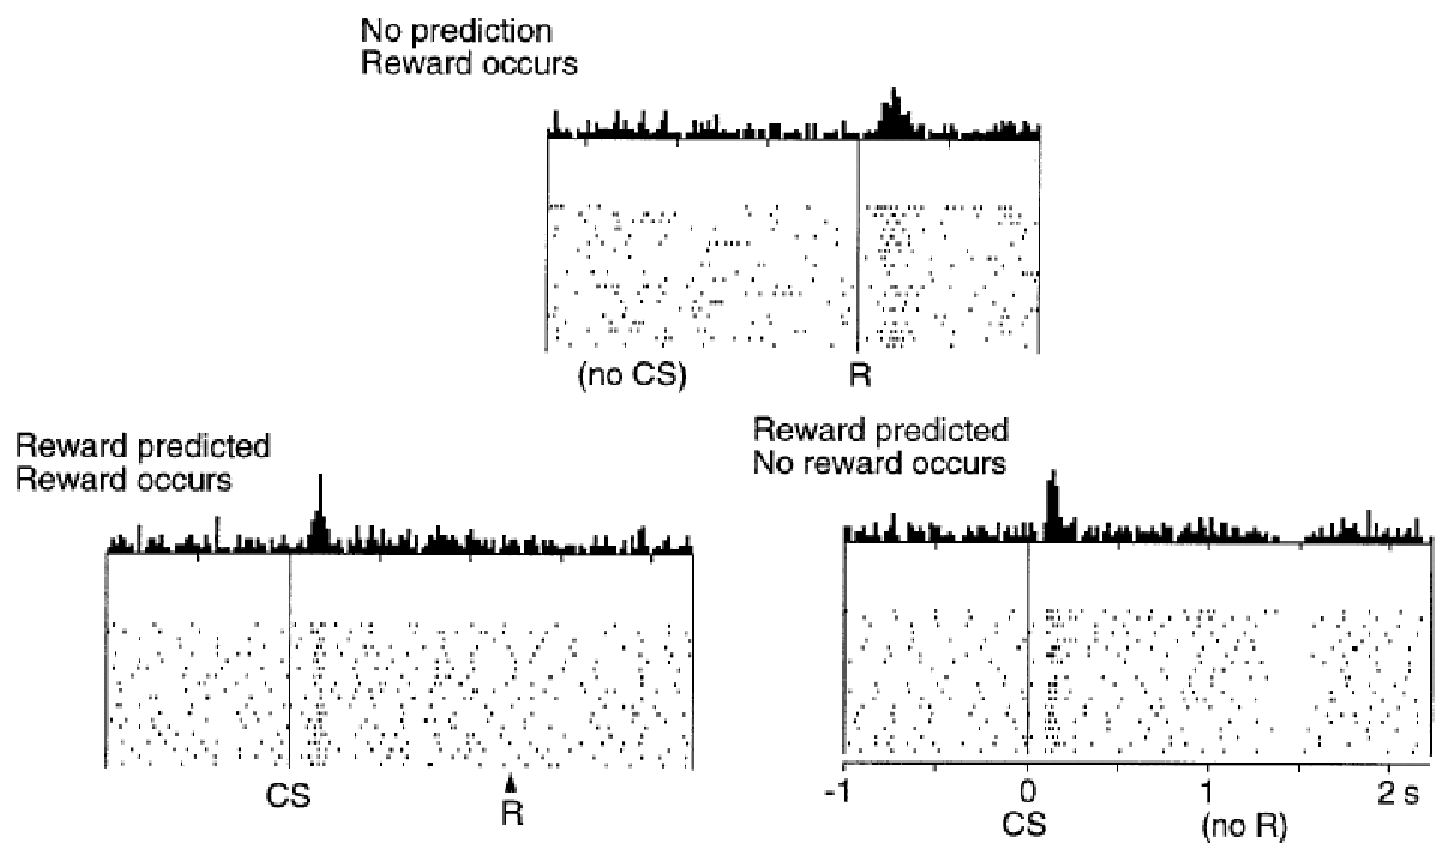
\includegraphics[width=15cm]{figures/schultz}
% \caption{Firing rates of midbrain dopamine neurons of the basal ganglia during classical conditioning (Adapted from Schultz et al., 1997)}
% \label{schultz}
%\end{figure}


%\bigskip

%\subsection{Computational Models of PFC}
%Our work builds on previous computational modeling work of formal accounts of DA's affect on PFC functioning.  The effect of DA is formalized by equating the firing rate of midbrain DA neurons to the key variable, the TD Error, of the powerful TD learning algorithm.  Using this connection between biology and machine learning, researchers have been able to provide models of how motor systems can learn sequences of overt actions leading to reward.  One of the primary insights of some recent models of PFC functioning is that the DA based TD learning mechanism might be used to learn, from experience, when to robustly maintain current representations in the PFC versus allowing updating to occur~\cite{BraverTS:2000:Control}.  As described earlier, it is helpful to think of the maintenance versus updating of PFC in terms of a gating mechanism.  When the gate is closed, the PFC representations are robustly maintained and protected from interference.  When the task contingencies change, the gate can be opened to allow for a more useful PFC goal or rule to be maintained to influence further processing.  The key insight is that, if TD can be used to learn sequences of \emph{overt} actions, it might be possible to use this same error signal to learn \emph{covert} actions, such as when to open and when to shut the gate on PFC representations.  By building computational models of PFC function, researchers have shown that this account is plausible~\cite{BraverTS:2000:Control,OReillyRC:2002:IDED}.  A layer of processing units representing  the PFC is included in these models, and this layer is used to actively maintain abstract task dimensions across the firing patterns of the units.  For instance, the PFC layer can encode, and actively maintain, a representation such as ``pay attention to the color of the stimuli''.  This maintained pattern of activity can then provide a ``top-down'' bias or up-modulation of pathways in posterior brain areas associated with the processing of stimulus color~\cite{CohenJD:1990:Stroop}.  The extra biasing provided by the PFC can be used to drive weaker, less automatic, behaviors (e.g. naming the color as opposed to reading the word in the Stroop task) when appropriate.  This activation based modulation is thought to be key to our ability to provide cognitive control over behavior~\cite{CohenJD:1992:Schizophrenia}.  The DA based adaptive gating mechanism can be used, within this context, as a way to signal to PFC when it is appropriate to strengthen the maintenance of the representation currently encoded (i.e. close the gate).  This occurs when a positive TD Error arises, signifying a positive change in expected future reward.  In other words, when the system is doing better than expected, close the gate on PFC representations so we are more likely to keep doing the same thing.  Conversely, when the network starts performing worse than expected, possibly due to task contingencies changing, this will result in a negative TD Error, signaling that the system is not performing as well as expected, and indicating that the system should adapt its behavior to perform more optimally.  The negative TD error can be used as a gating signal on the PFC representations, signaling the gate to open, allowing a new representation to replace the old, thereby allowing the network to flexibly adjust its control over behavior.
%
%Along with providing a neural mechanism that can learn to appropriately and adaptively gate PFC representations, these models have also been successful in tying frontal disturbances, such as those found in schizophrenia, to deficits in cognitive control~\cite{CohenJD:1992:Schizophrenia} and cognitive flexibility~\cite{BraverTS:1999:Schizophrenia,OReillyRC:2002:IDED}.  A recent elaboration of this model, XT~\cite{RougierNP:2005:XT}, is the first neuroscientific model able to provide quantitative fits to a hallmark task of cognitive control, the Stroop task, and a widely used measure of cognitive flexibility, WCST, in both neurologically intact and frontally damaged people.  
%In the next chapter, XT has been adapted to investigate whether a dysfunctional DA based gating mechansim can capture the specific executive profile of people with autism in WCST and Stroop.  




\section{General Modeling Approach}
\label{section:approach}

%
% General Modeling Approach
% 

This work focuses on using the methods of computational cognitive neuroscience to demonstrate how changes in PFC/DA interactions, leading to difficulties in updating PFC representations, can explain a broad array of behavioral patterns observed in autism. One reasonable strategy would involve the fabrication of a single complex biological model that is capable of performing all of the laboratory behaviors of interest, showing that this model matches the behavior of typically developing people but produces the behavioral patterns observed in ASD when it is modified to include PFC/DA dysfunction. Unfortunately, the range of relevant behaviors is broad, making the production of a single model capable of all of the behaviors of interest untennable.

As an alternative, we have pursued a strategy that builds directly upon the rich existing modeling literature. Separate previously published models, each successful in capturing behavioral patterns in a particular domain, were modified in a manner that reflects our general hypothesis that PFC/DA interactions are disrupted in ASD so as to reduce flexibility in PFC updating. In each case, we have found that hindering PFC updating causes the modified model to produce patterns of performance seen in ASD. It is important to note that no additional mechanisms were introduced into any of the previously published models. Only their existing, previously justified, mechanisms for cognitive flexibility were manipulated in order to capture the behavior of people with autism. Using this approach, we can show how cognitive inflexibility, arising from improper DA modulation of PFC, can account for a wide variety of behavioral phenomena observed in autism, including executive dysfunction, deficits on implicit learning tasks, problems with word sense disambiguation, and reduced prototype formation.




\section{Executive Dysfunction}
\label{section:executive}

%
% Executive Dysfunction
%

\section{Executive Task Performance}

People with autism are impaired at a variety of tasks involving planning~\cite{BennettoL:1996:AutismPlanningWCST}, flexibly adaptation of behavior~\cite{BennettoL:1996:AutismPlanningWCST,Ozonoff:1999:AutismStroopWCST}, and spontaneous generation of novel behaviors~\cite{TurnerW:1999:AutismGenerativity}. Tasks of this kind have been associated with executive control processes. This has led some researchers to view executive dysfunction as a central feature of autism~\cite{HughesC:1994:AutismExecutiveDysfunction}.
% Indeed, the Executive Dysfunction (ED) theory of autism seeks to explain many of the behavioral patterns exhibited by these individuals in terms of a failure of executive control over behavior

%There is extensive evidence that the prefrontal cortex plays an
%important role in executive control.  Along with the central claim of
%ED, this suggests that the root cause of many autistic behavioral
%patterns may lie in abnormalities in this region of the brain.  
%This is an interesting hypothesis because, while substantial progress has
%been made in many areas of autism research, no consensus has been
%reached concerning the neural basis of the disorder.  This view of ED
%suggests that the irregular development of prefrontal cortex may
%underly the patterns of cognitive performance seen in autism.

A more detailed examination of autistic behavior reveals that not all forms of executive processing are impaired, however. A perplexing aspect of the ASD executive profile is that cognitive flexibility is impaired while fundamental cognitive control remains relatively unaffected. Cognitive control describes the ability to enact a behavior in the presence of a distracting or more automatic competing response. In contrast, cognitive flexibility is the ability to fluently adjust cognitive control as contingencies change. A classic measure of cognitive control is the Stroop task~\cite{StroopJR:1935:Interference}, and a common measure of cognitive flexibility is performance on the Wisconsin Card Sort Test (WCST)~\cite{BergEA:1948:WCST}. Persons with autism have been shown to exhibit poor WCST performance, but they exhibit no more interference on the Stroop task than healthy controls~\cite{Ozonoff:1999:AutismStroopWCST}. This dichotomy challenges the notion that autistic behavior is the result of a global impairment of executive processes.
%, perhaps mediated by frontal abnormalities.

A second challenge appears in the developmental trajectory of executive deficits in autism. In young children with autism, executive abilities are intact when compared with controls matched for age and verbal ability~\cite{GriffithEM:1999:AutismYoungED}. Differences in cognitive flexibility arise over the course of development.
%, calling into question the role of ED in the etiology of autism.  
%Any theory intending to explain executive dysfunction in autism must account for
%the relative ``strengths'' and ``weaknesses'' that have been observed,
%as well as for this lack of observable deficits early in development.

These behavioral findings can be explained by positing separate mechanisms for cognitive control and for the flexible adaptation of control. In autism, the mechanism for control may be intact, but the flexibility mechanism may be compromised. Interestingly, this segregation of function is captured by the \emph{Cross-Task Generalization Model (XT)}~\cite{RougierNP:2005:XT}. Driven by broad neurocomputational considerations, XT casts PFC as central to cognitive control, while PFC/DA interactions mediate cognitive flexibility.
%XT has been used to capture the performance of both frontally damaged individuals and healthy controls on both the Stroop task and WCST~\cite{RougierNP:2005:XT}.

%In this section, we demonstrate that XT also offers a possible explanation for
%the executive processing profile exhibited by persons with autism.
%Specifically, we have found that simply weakening the influence of DA
%on PFC in the model is sufficient to both qualitatively and
%quantitatively capture autistic performance on both Stroop and WCST.
%This computational modeling result suggests that executive deficits in
%autism may be mediated by PFC/DA interactions.  Importantly, XT is a
%learning model, in which the development of neural representations and
%associated behavioral performance can be tracked as the model matures.
%Leveraging this property of XT, we show that the late appearance of
%executive deficits might be explained by the late maturation of PFC
%representations and PFC/DA interactions.  According to the model,
%early performance is driven largely by non-frontal, more posterior,
%brain systems which are largely unaffected by the posited DA-related
%abnormalities in autism.  As the PFC becomes more effective,
%differences in PFC/DA interactions are unmasked.

%\subsection{Modeling Prefrontal Cortex} 
 
%\subsection{Gating in the Prefrontal Cortex} 
% This is described in the background / introduction
%Under some accounts, cognitive control is enacted via the active maintenance of abstract rule-like representations in PFC.  These sustained PFC representations provide a top-down task-appropriate processing bias to more posterior brain areas~\cite{CohenJD:1990:Stroop}.  Computational analysis of these neural circuits have shown that active maintenance and the flexible adaptation of control are at odds, with the mechanisms that maintain PFC representations acting as an obstacle to the rapid updating of PFC contents. Thus, in order to achieve flexible behavior, a separate mechanism is needed to intelligently and rapidly update the actively maintained PFC control representations.  This can be seen as a ``gating'' mechanism, toggling between a state of maintenance and a state of updating, as appropriate for the task.  XT suggests that the gating decision is learned from experience, and this learning process critically involves the midbrain dopamine system, reified as the TD learning algorithm~\cite{BraverTS:2000:Control,RougierNP:2005:XT,BartoAG:1994:TDLearning}.

%As described earlier, the PFC has been broadly implicated in cognitive control and cognitive flexibility~\cite{Stuss:2000:WCSTLesion,Stuss:2001:StroopLesion}.  Under some accounts, cognitive control is enacted via the active maintenance of abstract rule-like representations in PFC.  These sustained PFC representations provide a top-down task-appropriate processing bias to more posterior brain areas~\cite{CohenJD:1990:Stroop}.  Biologically, the active maintenance of frontal control representations is supported by dense patterns of recurrent excitation in the PFC, as well as intrinsic maintenance currents~\cite{Goldman-RakicPS:1987:PFC_Maintenance}.  Computational analysis of these neural circuits have shown that active maintenance and the flexible adaptation of control are at odds, with the mechanisms that maintain PFC representations, and protect them from distracting inputs, acting as an obstacle to the rapid updating of PFC contents in response to shifting contingencies.  Thus, in order to achieve flexible behavior, a separate mechanism is needed to intelligently and rapidly update the actively maintained PFC control representations in a task appropriate manner.  This can be seen as a ``gating'' mechanism, toggling between a state of maintenance and a state of updating, as appropriate for the task.  XT suggests that the gating decision is learned from experience, and this learning process critically involves the midbrain dopamine system, reified as the TD learning algorithm~\cite{BraverTS:2000:Control,RougierNP:2005:XT,BartoAG:1994:TDLearning}.

\subsection{The XT Model} 

%\begin{figure}[ht]
%\begin{center}
%	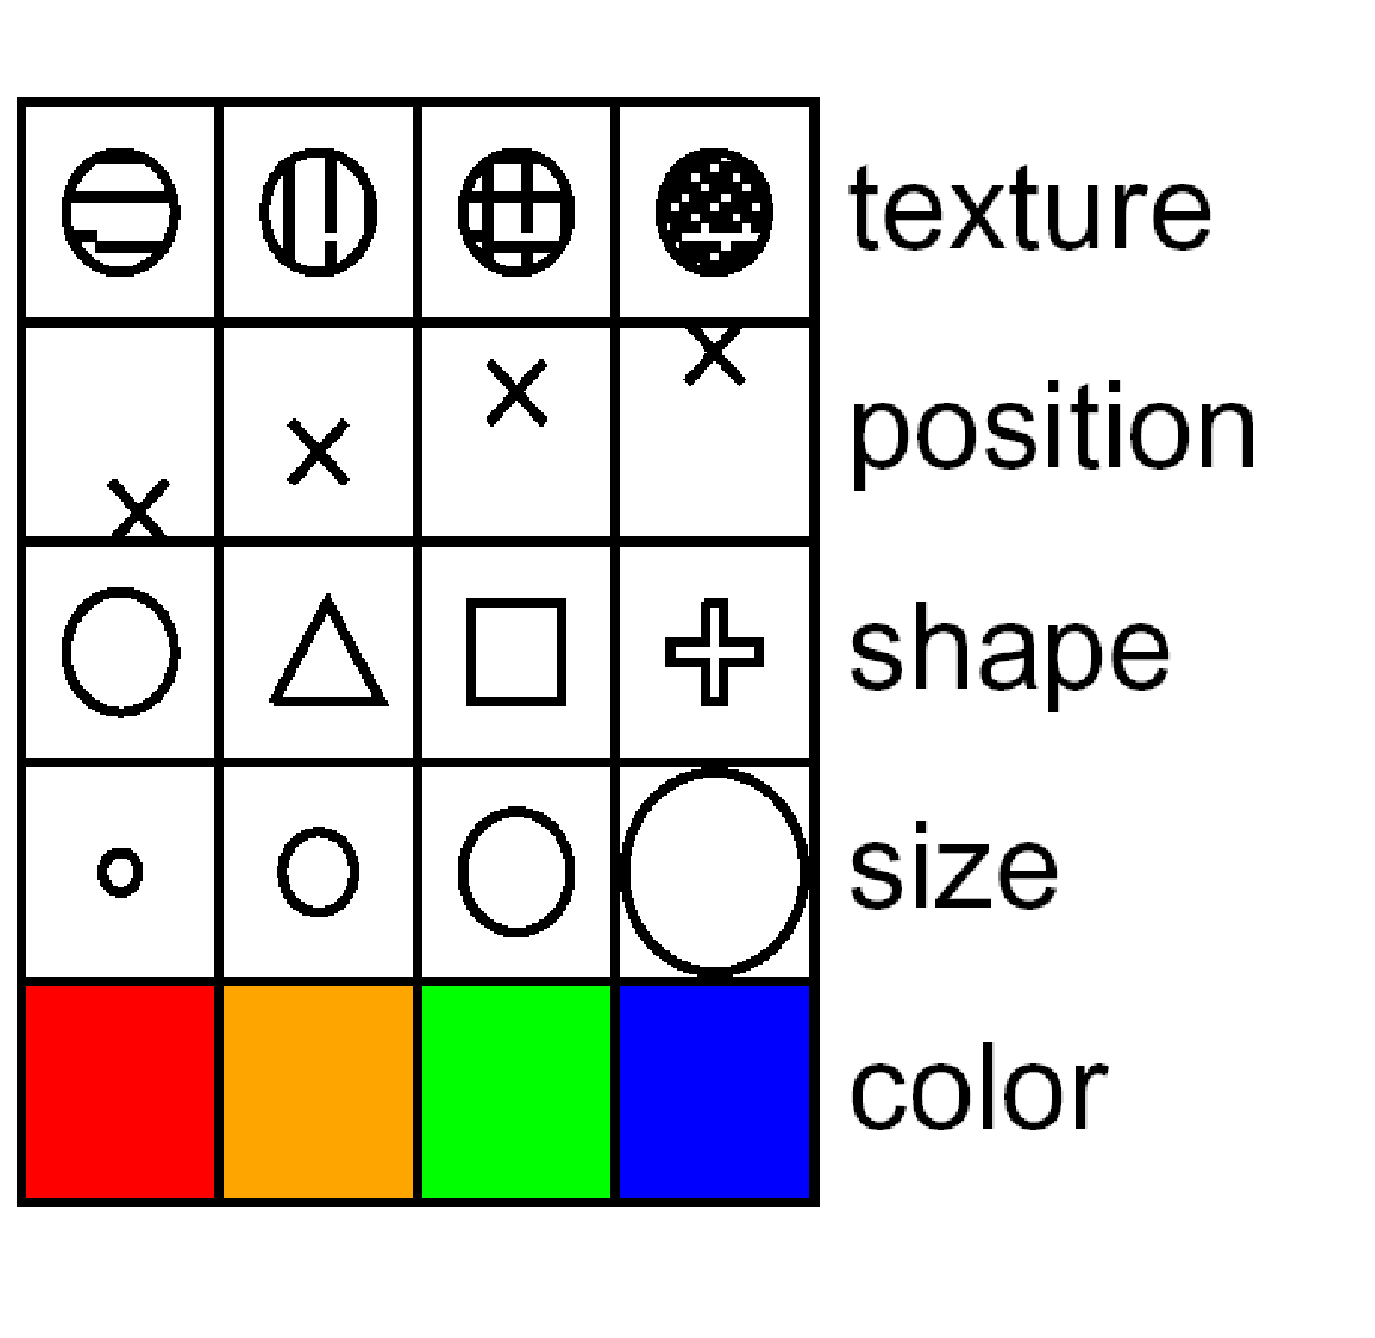
\includegraphics[width=42mm, height=35mm]{figures/xt_stim_layer2.eps}
%\end{center}
%\caption{Stimulus Input Layer: Caricature of input to the XT model, with rows portraying stimulus dimension (color, shape, size, etc) and columns indexing feature values across dimensions (small, medium, large, etc.)}
%\label{stimuluslayer-figure}
%\end{figure} 

The architecture of the XT model is shown in Figure~\ref{xt-layout-figure}. This model makes use of the Leabra framework~\cite{OReillyRC:2000:Computational}. The input of XT consists of two layers of neural units used for the presentation of up to two stimulus objects. It is natural to think of the rows of each input layer as representing different dimensions (e.g., color, shape, texture) and the columns indexing features across each dimension (e.g., red, orange, green, blue). The Response layer has essentially the same structure as an input layer, but includes one additional unit, which codes for ``no response''.  

\begin{figure}
\begin{center}
	\includegraphics[width=125mm]{figures/xt_arch_2.ps}
\end{center}
\caption{XT Model Architecture. The upper left corner shows a
         caricature of the input to the XT network, with rows
         portraying stimulus dimension (color, shape, size, etc.) and
         columns indexing feature values across dimensions (small,
         medium, large, etc.). The AG unit implements ``adaptive gating'' 
	 by modeling the effects of DA on PFC.}
\label{xt-layout-figure}
\end{figure} 

A collection of Hidden layers map from stimuli to responses. Activity in these layers can be modulated through top-down biasing signals from an actively maintained representation in the PFC layer. Unlike previous models, the actively maintained representations in PFC are learned through a developmental process that involves training the model to perform a variety of simple tasks. These tasks share a need to selectively attend to individual dimensions of the stimuli. The standard synaptic plasticity mechanisms of the Leabra framework, applied over the course of developmental training, gives rise PFC representations that support focusing attention on a single stimulus dimension at any one time~\cite{RougierNP:2005:XT}.

The Task input indicates which task is to be performed, with one input unit coding for each task. The Dimension Cue layer is used to indicate the currently relevant stimulus dimension, with each unit in the layer corresponding to a specific stimulus dimension. All of the input units are turned off for tasks in which the model must discover the relevant stimulus dimension on its own.

The flexible adjustment of cognitive control is implemented using a DA-based adaptive gating (AG) mechanism. The model receives a positive scalar reward signal whenever it produces a correct response, and the AG calculates the change in expected future reward: the TD Error. Importantly, the AG, modeling phasic DA responses, not only modulates the learning of reward expectation but also manipulates the ``gate'' on PFC. When the model performs better than expected the current PFC representation is strengthened. When the model performs worse than expected the current PFC representation is destabilized, allowing a new, possibly more appropriate PFC representation to be entertained~\cite{RougierNP:2005:XT}.

%In the model, the \begin{math}\delta(t)\end{math} value directly modulates excitatory ionic maintenance currents (\begin{math}g_m\end{math} below).  Large maintenance currents drive the membrane potential of simulated neurons in the PFC up, pushing them towards their maximal firing rate.  These currents are not allowed to become negative, being clipped at zero instead.  The maintenance currents, $g_m$, of simulated neurons in PFC are computed by:

%\begin{equation}g_m(t-1) = 0 ~if~ |\delta(t)| > \theta\end{equation}
%\begin{equation}g_m(t)_j = g_m(t-1) + \delta(t) a_j\end{equation}
%\begin{center}$where~a_j~is~the~current~activation~value~of~PFC~unit~j$\end{center}

%Therefore, a positive \begin{math}\delta(t)\end{math} will result in an increase in active maintenance of PFC representations, while a negative \begin{math}\delta(t)\end{math} will destabilize PFC.  The value \begin{math}\theta\end{math} represents a threshold value for the ionic currents.  If the TD error, \begin{math}\delta(t)\end{math}, exceeds this amount (\begin{math}\theta = .5\end{math} in all simulations), then the maintenance currents, \begin{math}g_m\end{math}, are effectively reset.  Over time, the network learns to maintain PFC representations that are likely to result in reward.  


%XT is the first computational cognitive neuroscience model to explore
%the development of PFC representations, and it is the first to provide
%good quantitative fits to both Stroop and WCST data, for both
%neurologically intact and frontally damaged people, based on a biologically informed architecture.

%\subsection{Modeling Autism Using XT}

\subsection{Modeling Autism Using XT}

% \subsubsection{General Approach}

Our theory suggests that a deficit in DA functioning can account for the impaired cognitive flexibility seen in people with autism, while leaving cognitive control robust and relatively unaffected. We have tested this theory by reducing the effect of the DA signal in the XT model by scaling the TD Error (AG) by a constant factor, $\kappa$. The model of typically developing individuals uses $\kappa = 1$, and autism is modeled using $\kappa < 1$. This scaling of the TD Error by $\kappa$ is the only modification from the original XT model that we made. A $\kappa$ value of $0.54$ was found to produce the best fit to human performance. This reduction of the DA signal decreases the efficacy of the PFC gating system, resulting in less efficient destabilization of PFC when errors are made.
%The scaling was only used to modulate the simulated maintenance currents within the PFC layer, and not used to modify the learning of the weights into the Adaptive Gating unit.  An important point of future work is to also test the effects of this manipulation on these weights, weakening the overall influence that dopamine has on learning within circuits involved in the computation of future expected reward, as well.  

%It is worth noting that the modeled DA signal remains agnostic as to the precise quantitative nature of actual DA levels.  It is possible, for instance, that a optimal firing rate of the midbrain DA neurons exists for efficient PFC gating.  This implies \emph{either} too much or too little DA could have deleterious results on the effectiveness (a lower $\kappa$ value) of the DA based PFC gating system.

\subsection{Modeling WCST} 

%The WCST consists of a deck of cards, which contain stimuli varying along three dimensions (e.g., color, shape, quantity) and across four different features per dimension (e.g., for color dimension: red, orange, green, \& blue).  Participants are told to sort the cards into piles, but they are not given any instructions concerning how to do this correctly.  Instead, only sparse feedback ---``Correct'' or ``Incorrect''--- is given upon the placement of each card, until the proper sorting strategy is discovered.  After the sorting rule (e.g., sort by color) is learned by the participant, and $10$ consecutive correct sorts are accomplished, the rule is changed without informing the subject.  This procedure repeats until either $6$ correct categories (sets of $10$ correct consecutive sorts) are achieved, or all $127$ cards in the deck are exhausted.  Errors are recorded as incorrect sorts, with perseverative errors scored as an incorrect sort that used the last correct sorting rule.  Success at WCST requires the ability to flexibly change the dimension being maintained by PFC as the sorting rules change.  Modeling WCST in the XT framework required use of only three of the five possible input dimensions.  The same methods for administrating WCST to human participants were used in these simulations.

\begin{figure}
  \begin{center}
  \resizebox{8cm}{!}{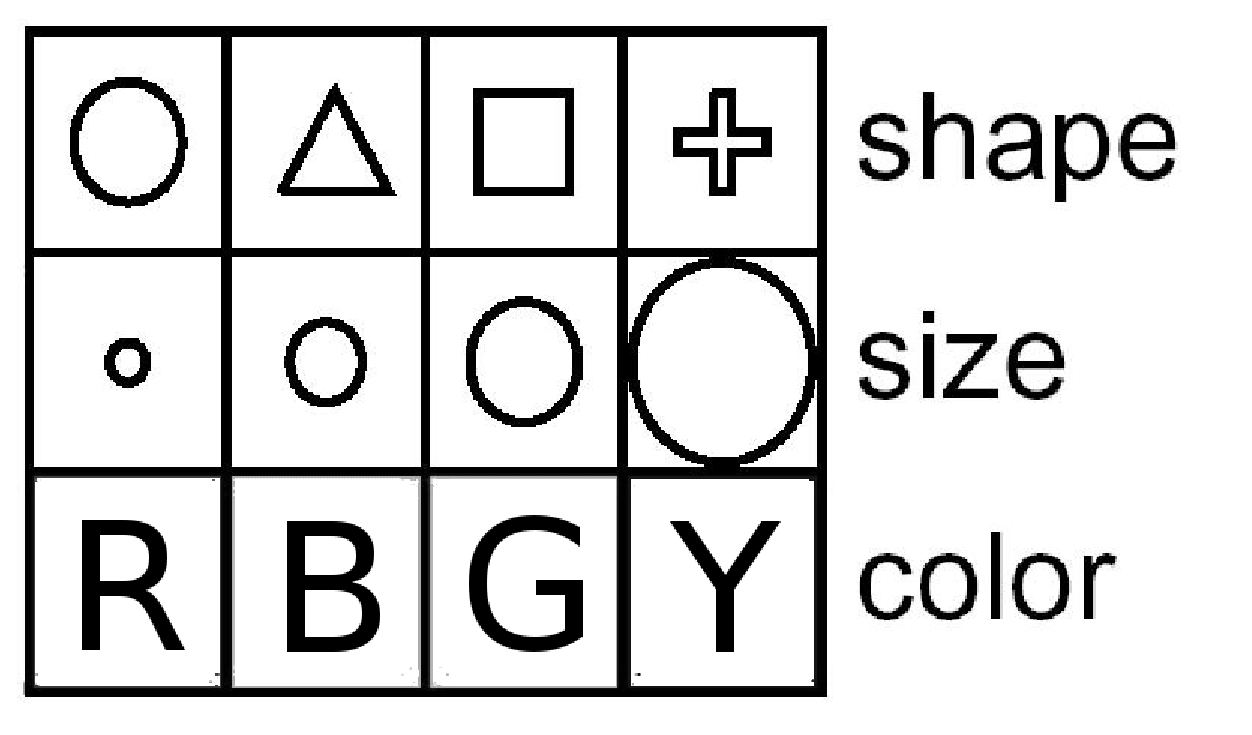
\includegraphics{figures/xt_wcst_stim}}
  \end{center}
  \caption{XT WCST example stimulus input}
  \label{xt_wcst_stim}
\end{figure}

As in the original XT work, each trial of the WCST was modeled by presenting a single stimulus object ``card'' at the model's inputs, with one unit activated for each feature of the stimulus across three stimulus dimensions. (See Figure~\ref{xt_wcst_stim}.) The model ``sorted'' the ``card'' by outputing the feature of the current stimulus relevant for sorting. For example, when cards were to be sorted by color, the model was expected to output the color of the stimulus (e.g., ``red''). Importantly, the model was not instructed concerning the sorting rule (i.e., the Dimension Cue inputs were all off). Thus, the model needed to search for the relevant stimulus dimension. The model received a positive scalar ``reward'' signal when its output was correct. The use of TD learning to produce AG activity, along with the top-down modulation from PFC, allowed XT to successful learn to focus on the relevant stimulus dimension. The AG mechanism strengthened the maintenance currents of modeled PFC pyramidal cells during good performance, causing the active maintenance of the sorting rule in PFC. When the sorting rule was switched, the actively maintained PFC representation became invalid. Continued active maintenance of PFC firing rates would result in perseverative errors. In the standard XT model, the AG alleviated this problem by providing a gating signal to PFC when reward was expected but not delivered, allowing PFC contents to change~\cite{RougierNP:2005:XT}.

%Four main measures were used in evaluating the performance on the WCST task:

%	1. Total Number of Errors
%
%	2. Percentage of Total Errors 
%
%	3. Total Number of Perseverative Errors
%
%	4. Percentage of Perseverative Errors

%In the XT framework, the Dimension Cue layer is used to inform the network what dimension is currently relevant.  By *not* using this cue, the network is left to figure out what the sorting rule is by feedback alone, analogous to participants in WCST.  Only three of five possible dimensions where used in the stimulus layer in order to facilitate a tighter link with the model to that of the actual WCST task.  

\subsection{Modeling Stroop} 

%Stroop tests cognitive control by measuring the ability to inhibit a prepotent response.  In Stroop, the stimuli are different words presented in various colored fonts.  Participants are asked to either read the word or to name the color of the font in which the text is presented.  People are faster overall at reading the word as opposed to naming the color of the word.  Furthermore, when comparing the neutral (e.g., the word ``house'' in red font) versus the incongruent (e.g., the word ``green'' written in red font) conditions, people are slower in the incongruent case for color naming, but not for word reading.  This is known as Stroop interference.

%Cohen and Servan-Schreiber~(1990)\nocite{CohenJD:1990:Stroop} provided a computational account of the Stroop task. This model incorporated multiple associative pathways from stimulus features to possible responses.  They used a stronger, more automatic word reading pathway through posterior cortex and a relatively weak color naming pathway.  In their model, a task representation, maintained in PFC, provided top-down biasing, injecting extra activity into the color naming pathway when doing so was necessary to overcome the prepotent word reading pathway (i.e., when asked to name the font color).  The resulting competition between the two strong pathways resulted in an increase in response time in the color naming incongruent condition.  Response time was not increased in the word reading incongruent condition, however, as the weaker color naming pathway, when unsupported by PFC, offered little competition.

The XT model performed the Stroop task in much the same way as Cohen's and Servan-Schreiber's seminal model~\cite{CohenJD:1990:Stroop}, leveraging competition between pathways of varying strength: the strong word reading pathway and the weak color naming pathway. In order to simulate this competetion, the frequency of trials in which one dimension (font color) was experienced during development was manipulated. The font color dimension was relevant only 25\% as often as the other dimension, word reading. The time needed for output activity to stabilize was taken as a response time measure~\cite{RougierNP:2005:XT}.
%The settling time, in ``cycles'', of the network was linearly scaled to ``milliseconds'' using a single free parameter, allowing a direct comparison between model results and human data.

\subsection{Simulation Results}

\subsubsection{Simulations} 
Due to stochasticity in model initial conditions and in the sequence of developmental trials, $100$ distinct network models were prepared using the XT training procedure, stopping when a performance criterion was reached, up to a maximum of $100$ training epochs.  Each network was tested under both conditions of DA modulation ($\kappa = 1$ for healthy networks and $\kappa = .54$ for networks modeling ASD), on both WCST and Stroop. Each of the $100$ networks was treated as an individual subject for the purposes of data analysis.

\subsubsection{WCST Results} 
WCST results matched data reported in the literature. The differences between simulated performance of normally functioning individuals and simulated autistic performance were statistically reliable ($p < 0.001$) and consistent with previous studies~\cite{PriorMR:1990:AutismWCST,Ozonoff:1999:AutismStroopWCST,MinshewNJ:2002:AutismWCST}. Specifically, perseverative errors, marking a failure to flexibly discard the initial sorting rule when it was no longer rewarded, were significantly more numerous in the reduced DA modulation version of XT. (See Figure~\ref{ed-results-figure}.)

\begin{figure}
\begin{center}
	\includegraphics[width=110mm]{graphs/wcst.ps}
                                                                
\textcolor{white}{\\--------------------------------\\}

	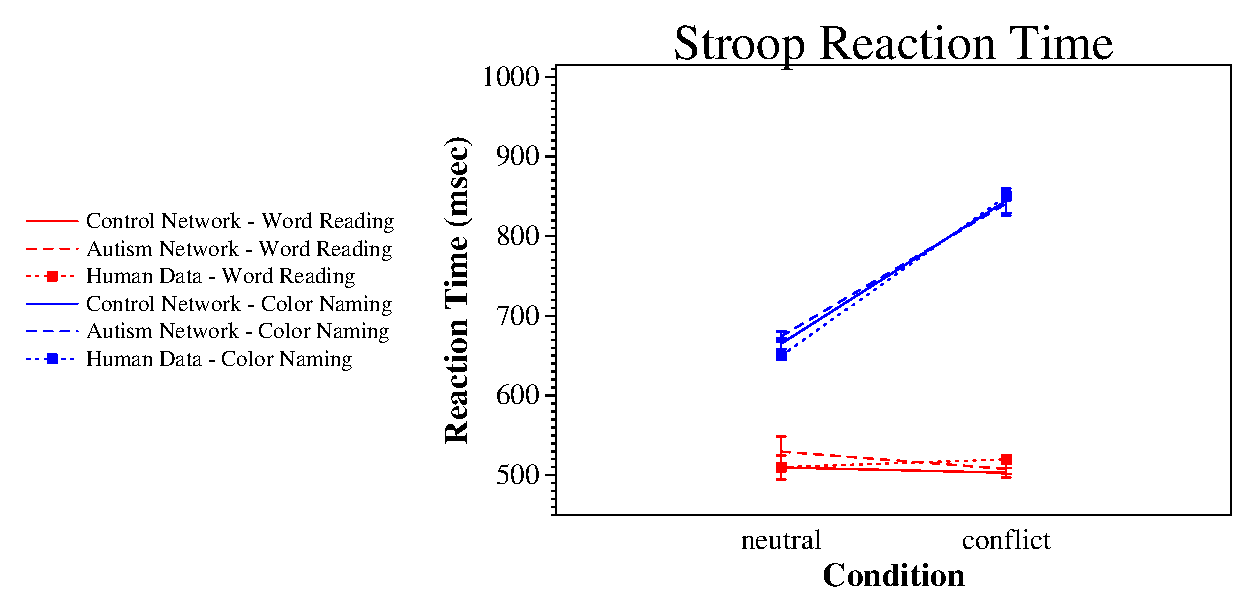
\includegraphics[width=110mm]{graphs/stroop.ps}
\end{center}
\caption{Top: Comparing performance on WCST perseveratitive errors for normally functioning and individuals with autism to data from Minshew et al., 2002. People with autism committing significantly more perseverative errors. Error bars are standard errors of the mean. Bottom: Stroop reaction time plot comparing the simulated autistic and normally functioning network's performance to human data. Healthy human data from~Dunbar et al.~(1984). Autistic subjects perform no differently than controls~(Ozonoff et al., 1999).} 
\label{ed-results-figure}
\end{figure} 

\subsubsection{Stroop Results} 
Model performance on the Stroop task provided a good quantitative fit to human performance. (See Figure~\ref{ed-results-figure}.) The model with intact DA function displayed the classic Stroop reaction time results --- slowing for conflict stimuli when color naming. The performance of the ASD model showed no significant increase in Stroop interference in comparison to the healthy model~($F(1,198) = 0.62$; $p > 0.43$), which is consistent with past findings~\cite{Ozonoff:1999:AutismStroopWCST}.

\subsubsection{Developmental Results}
These simulations involved the introduction of a DA deficit only after the model was fully developed. Thus, these simulations ignored the possibility that an early manifestation of a DA deficit might hinder the proper learning of PFC representations, introducing an impairment in cognitive control in the model that is not observed in autistic subjects. To address this issue, the DA deficit in the ASD model was introduced prior to developmental training. PFC development and model performance were analyzed over the entire developmental period of the model ($100$ epochs). Two groups of $10$ networks were used: an autistic group with $\kappa = 0.54$ and a control group with $\kappa = 1.00$. At the end of developmental training, the networks exhibited the same pattern of results as seen in the initial simulations. Furthermore, we found that the DA deficit did not hinder the learning of useful PFC representations, allowing for focused attention on a single stimulus dimension.

% Furthermore, careful examination of the development of the PFC representations provided some insight into why executive deficits might appear late in autism, as described in the literature~\cite{GriffithEM:1999:AutismYoungED}.  

% \subsubsection{PFC Representations} 

% Figures~\ref{rep1-figure} and \ref{rep2-figure} plot the synaptic strengths from the PFC layer to the Response layer.  Each large box corresponds to a PFC unit, and each encapsulated small box corresponds to a Response unit, with the strength of the connection from the given PFC unit to the given Response unit being reflected in the brightness of the box (lighter means stronger).  Note that each row designates connections to Response layer units representing features in the same stimulus dimension.  (See the upper left corner of Figure~\ref{xt-layout-figure}.)  Thus, these plots can be used to examine the degree to which the PFC layer developed a representational scheme that allowed for the selective modulation of individual stimulus dimensions.  For a given PFC unit (large box), a bright row of connections (small boxes) indicates that that unit selectively supports attention to the stimulus dimension corresponding to that row.  In Figure~\ref{rep1-figure}, which was generated early in developmental training, both the autistic network and the control network lack strong dimensional weights.  However, in Figure~\ref{rep2-figure}, both networks have developed strong dimensional representations in PFC, as evidenced by the extremely salient horizontal bands of ``strong'' weights.  Thus, appropriate PFC representations were acquired only slowly over the course of developmental training, and the DA manipulation did not hinder the formation of these representations.

% \begin{figure}[t]
% \begin{center}
% 	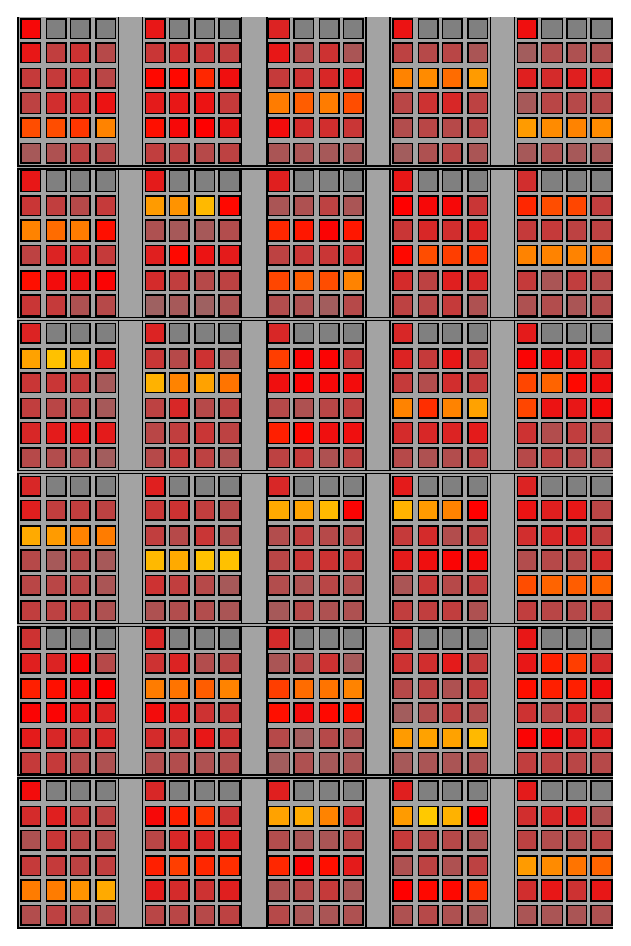
\includegraphics[width=35mm,height=55mm]{graphs/PFCwts1.05.eps}
% 	\hspace{18 mm}
% 	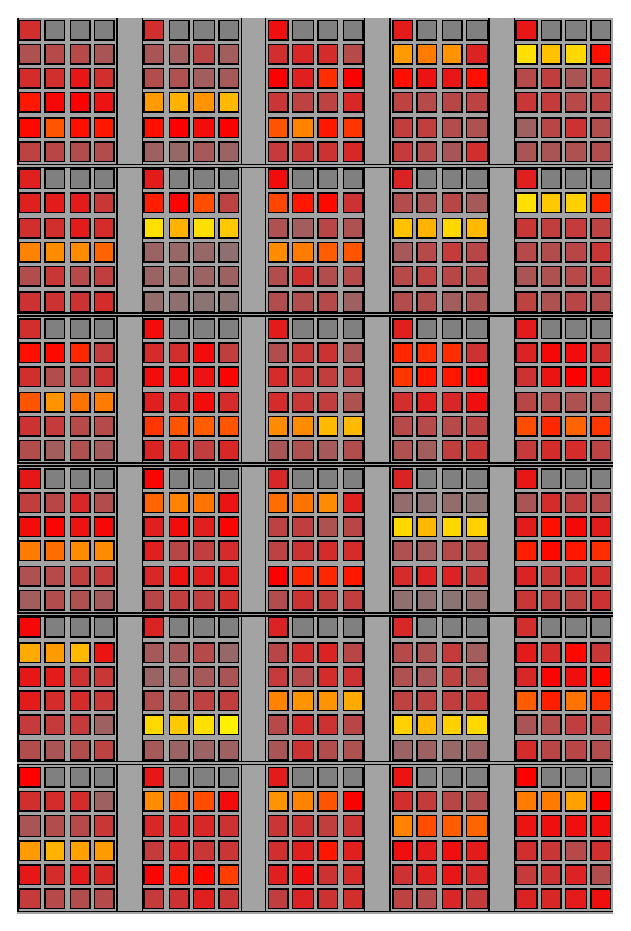
\includegraphics[width=35mm,height=55mm]{graphs/PFCwts54.05.eps}
% \end{center}
% \caption{PFC Representations early in development
%          (epoch 5): left - control model, right -
%          autism model.}
% \label{rep1-figure}
% \end{figure} 

% \begin{figure}[th]
% \begin{center}
% 	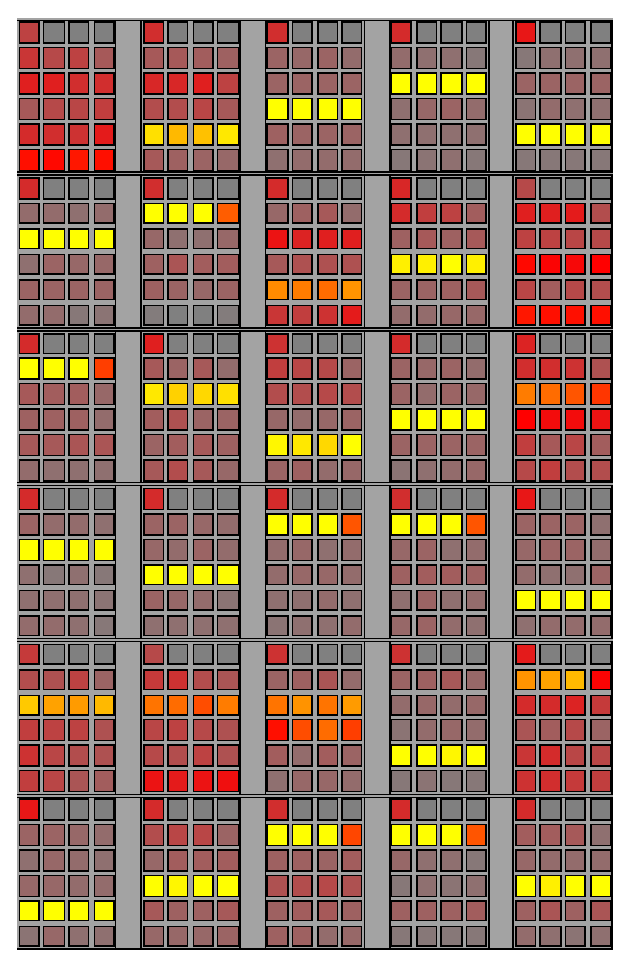
\includegraphics[width=35mm,height=55mm]{graphs/PFCwts1.100.eps}
% 	\hspace{18 mm}
% 	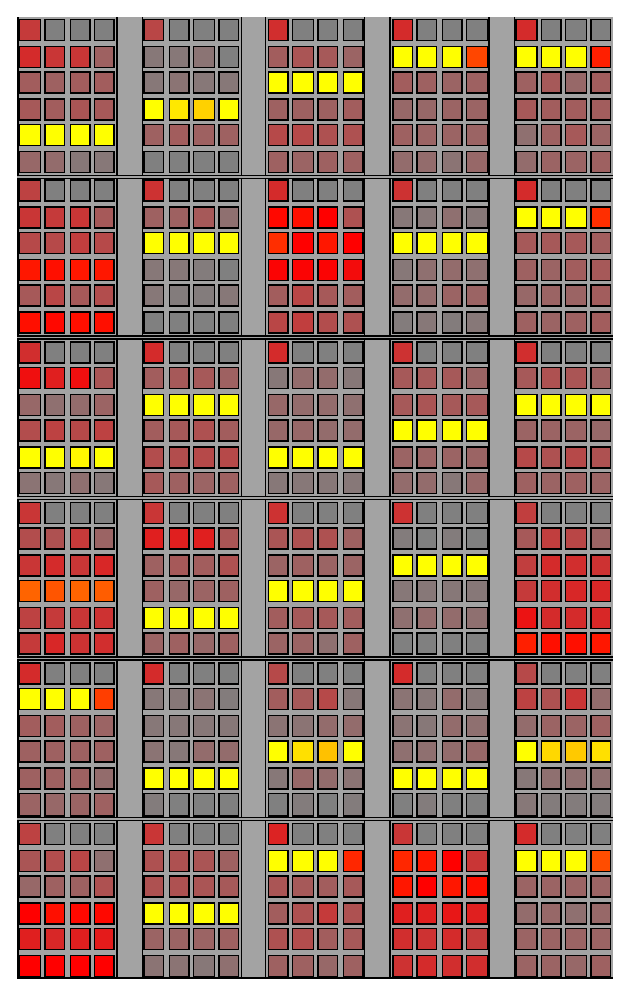
\includegraphics[width=35mm,height=55mm]{graphs/PFCwts54.100.eps}
% \end{center}
% \caption{PFC Representations late in development
%          (epoch 100): left - control model, right -
%          autism model.}  
% \label{rep2-figure}
% \end{figure} 

% \subsubsection{Executive Dysfunction Development} 

Interestingly, these simulations offer a potential explanation for the observation that cognitive flexibility deficits, in comparison to controls, appear late in development~\cite{GriffithEM:1999:AutismYoungED}. In Figures~\ref{stroop-devel-figure}~\&~\ref{wcst-devel-figure}, the Stroop interference effect and the number of perseverative errors in WCST are plotted over developmental training time. Figure~\ref{stroop-devel-figure} shows no effect of the DA manipulation across development. Stroop interference was significantly greater for the autistic networks during only $1$ training epoch out of the $100$ ($p < 0.003$), demonstrating robust cognitive control throughout development. Figure~\ref{wcst-devel-figure}, however, shows a significant difference in perseverative errors only after an initial period of developmental training. During the first $53$ epochs there was a significant difference ($p < 0.05$) during only $26.4\%$ of the epochs, but later in development (epochs $54-100$) a significant difference was reached $93.6\%$ of the time. Importantly, neither healthy nor autistic models showed a distinct advantage or disadvantage during the earliest stages of development. We conjecture that early poor performance by both model types was largely due to the fact that strong, dimensionally selective, PFC representations had yet to learned. Without such PFC representations, the networks were forced to rely more heavily on synaptic plasticity in the Hidden layers (posterior cortex) to perform the tasks. Later in development, both healthy and autistic networks acquired good PFC representations, but the models with reduced DA influence on PFC displayed difficulties in updating those representations when expected reward stopped being delivered (i.e., when the sorting rule was changed).

\subsection{Summary}

These simulations show that, given the XT account of the role of PFC in executive control, reducing the influence of DA on PFC adaptive gating is sufficient to capture the pattern of performance exhibited by people with autism on tests of cognitive flexibility (WCST) and cognitive control (Stroop). Furthermore, we demonstrated that weakening the DA signal over the course of PFC development continues to reflect autistic performance, while also providing some insight into the late appearance of cognitive flexibility deficits in autism. More information about these simulations may be found in Kriete \& Noelle~(2015).\nocite{KrieteT:2015:ED}

\begin{figure}[t]
\begin{center}
	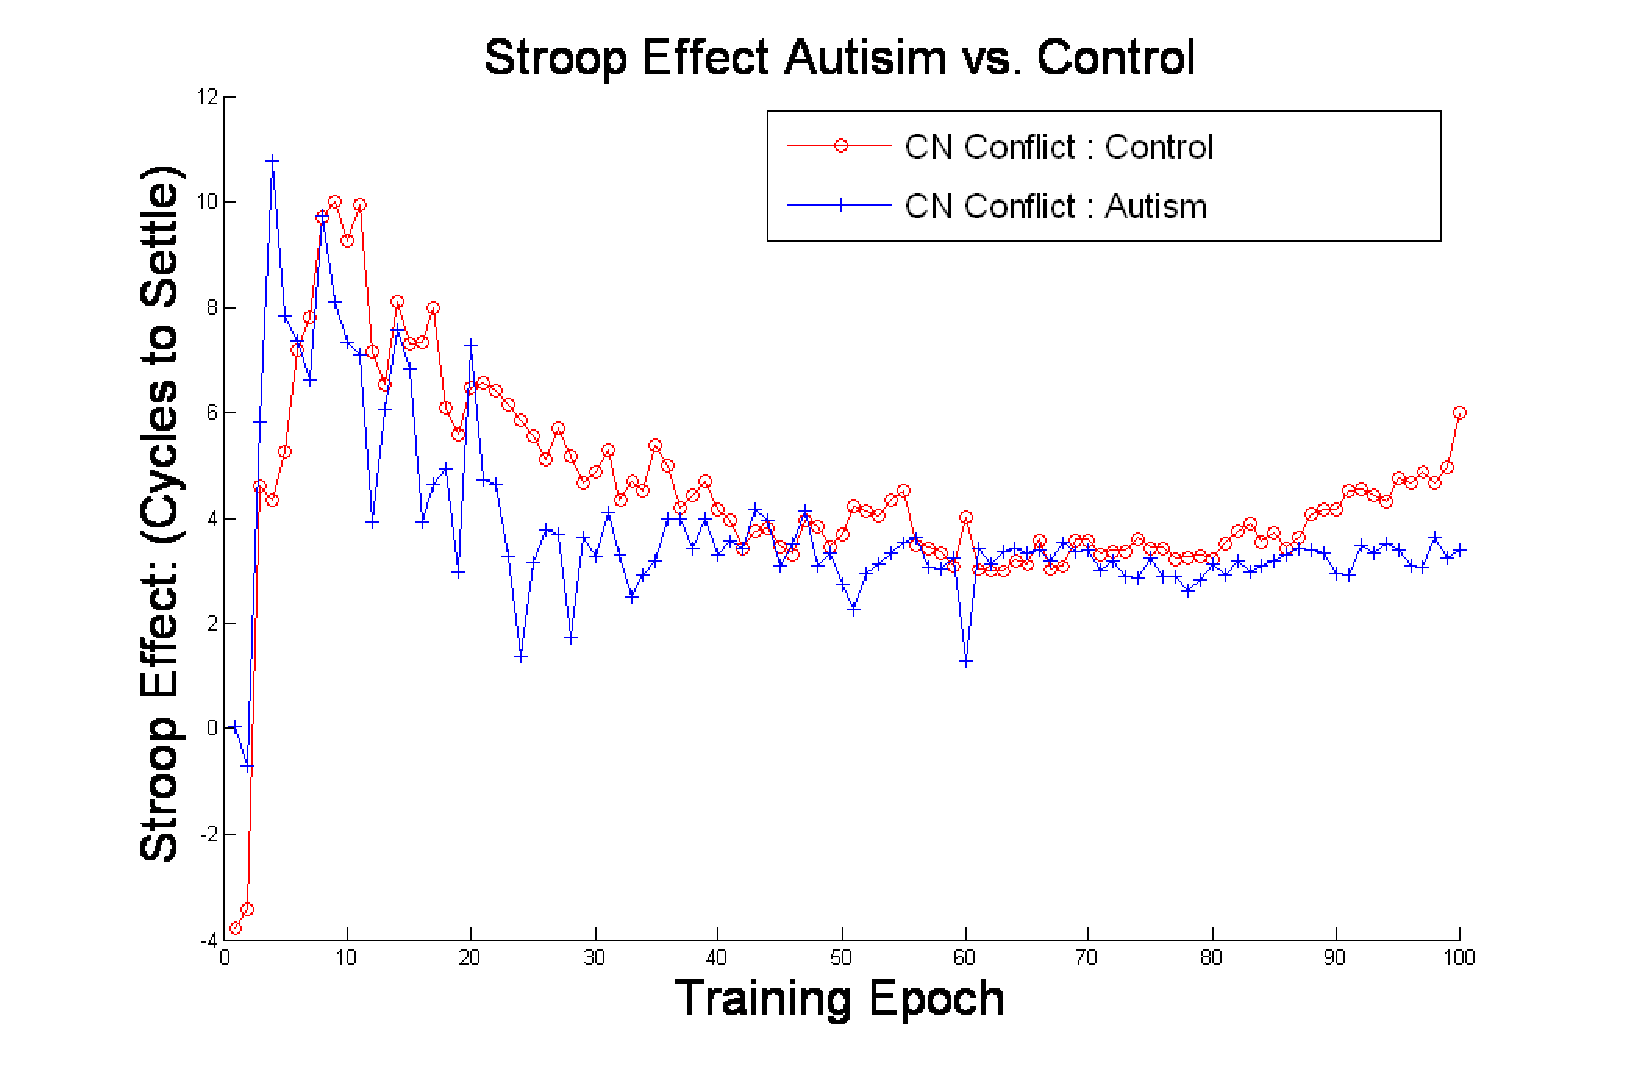
\includegraphics[width=145mm]{graphs/stroop_devel.eps}
\end{center}
\caption{Model Stroop Interference Over the Course of Development.} 
\label{stroop-devel-figure}
\end{figure} 

\begin{figure}[t]
\begin{center}
	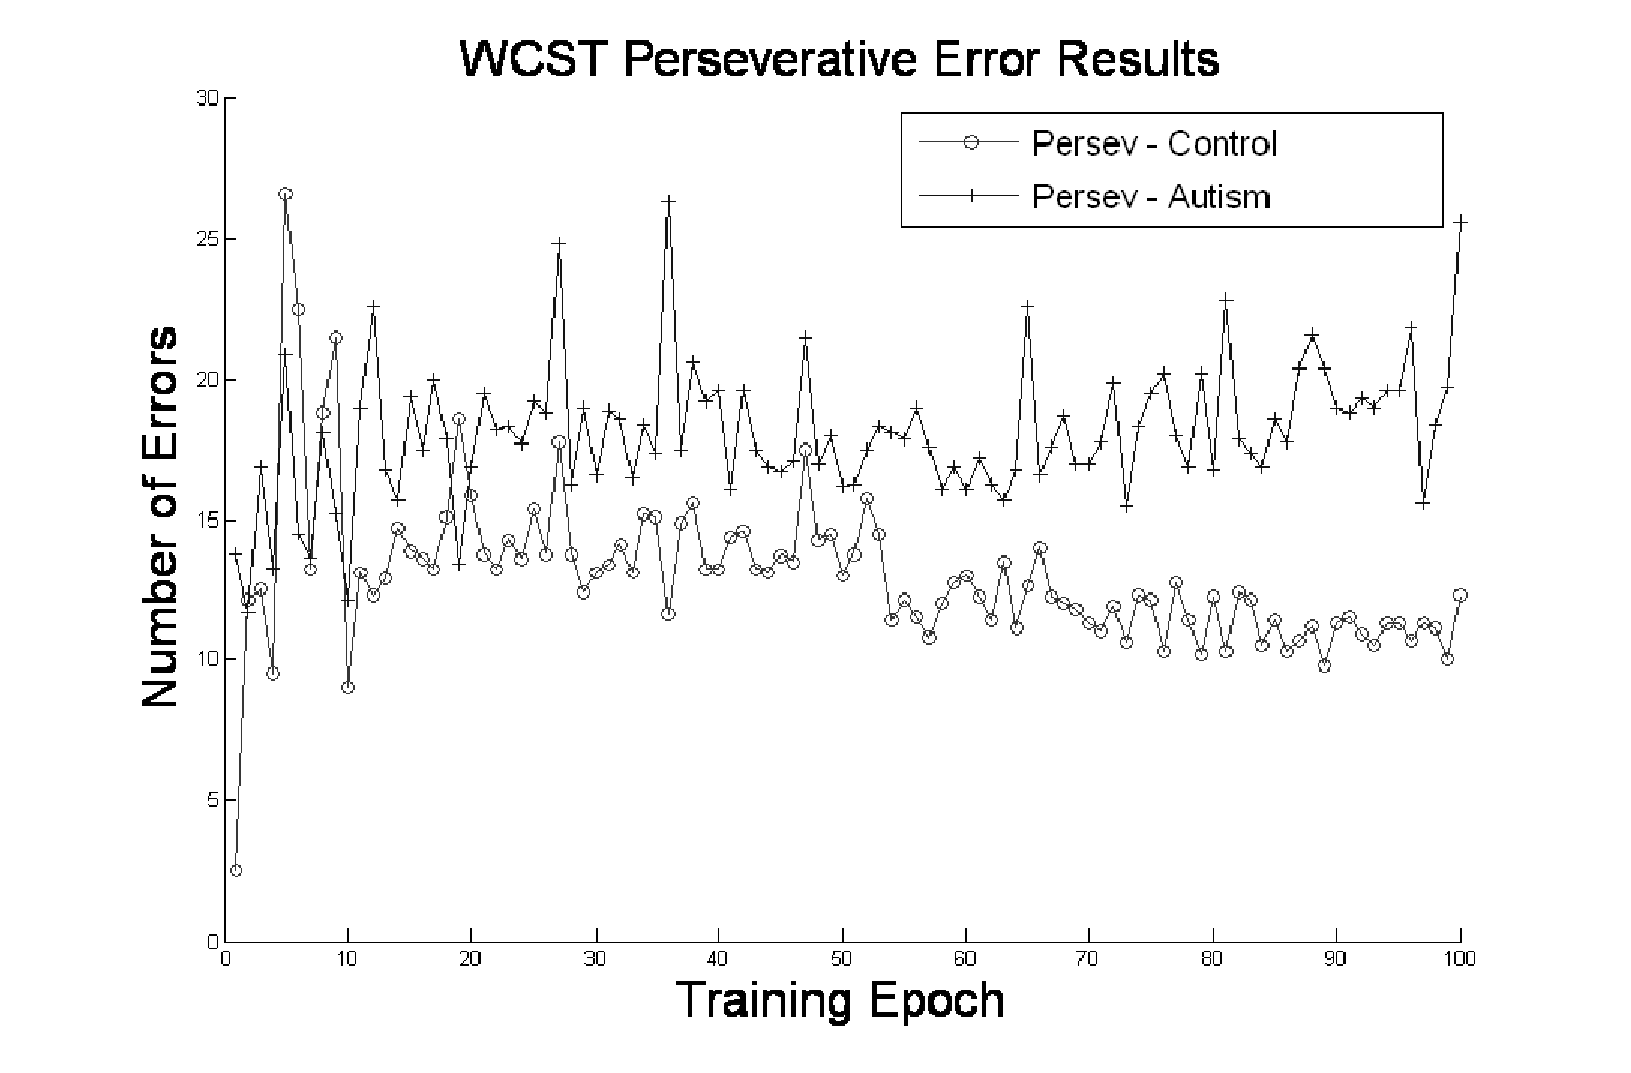
\includegraphics[width=145mm]{graphs/wcst_devel_persev.eps}
\end{center}
\caption{Model WCST Perseverative Error Count Over the Course of Development.} 
\label{wcst-devel-figure}
\end{figure} 




\section{Stimulus Overselectivity}
\label{section:overselectivity}

%
% Stimulus Overselectivity
%

%TEK we should expand our citations in this section before submitting

\subsection{Stimulus Overselectivity}
Various contemporary theories hypothesize that people with autism possess deficits in integrating contextual information in an appropriate manner.  Problems integrating information, it is argued, result in a processing style which highlights the specific pieces of the environment at the cost of more general high-level information~\cite{HappeF:1999:WCC}. This ``piecemeal'' style is capable of explaining an impressive variety of both the advantageous and detrimental behavior demonstrated by people with autism.  One possible mechanism that could give rise to information integration difficulties would be a tendency to restrict attention to an excessively small number of features, with difficulty in shifting attention to other features.  

Stimulus overselectivity, where a restricted set of components within a compound stimulus tend to dominate behavior, was first documented in the early 1970s in people with autism~\cite{LovaasO:1971:Selective}.  This effect has since been demonstrated both within and across different modalities as well as by varying the number of features composing the compound stimulus~\cite{ReedP:2005:TaskLoad}.  The paradigmatic task involves conditioning responses to a stimulus made of multiple, simultaneously presented, components.  After the initial association of the compound stimulus with reward/response, each individual component is tested separately, assessing the degree each has acquired control over the subject's behavior. (See Figure~\ref{OS-Task}.)  Normally developing individuals respond equally to all components.  People with autism, to the contrary, are more likely to respond to a single component, thus demonstrating overselectivity.  Overselective behavior in people with autism is a plausible explanation for the observed problems in generalizing learned behaviors to novel situations.  In such situations, restricted, often irrelevant, portions of the environment become tightly coupled with the performance of the desired behavior.  If this restricted portion is not consistently available to the individual, generalization to new settings will suffer.  This is a major focus of many behavioral and intervention techniques. 

\subsection{Cognitive Flexibility \& Overselectivity}
Our modeling work on executive dysfunction demonstrates how impaired interactions between the mesolimbic dopamine (DA) system and the prefrontal cortex (PFC) can result in perseverative attention to an overly restricted set of stimulus dimensions and features, as exhibited by perseveration in the WCST~\cite{KrieteT:2015:ED}.  Utilizing an abstraction of this same mechanism, in the following we show how show how an analagous perseverative attention mechanism results in a significant increase in stimulus overselectivity.   

%TEK Dave, I'm tempted to edit out the WM load from this section. What are your thoughts? 
An intriguing study suggests that stimulus overselectivity can be induced in healthy individuals by requiring the concurrent performance of a working memory task~\cite{ReedP:2005:TaskLoad} with overselectivity training consisting of learning a multi-component stimulus to response mapping.  Working memory tasks are widely believed to enlist the resources of PFC, providing additional support for the conjecture that healthy individuals utilize this area when performing this task.

\subsection{The Overselectivity Task}
An operant conditioning paradigm traditionally has been used when assessing the degree of overselective behavior in people with ASD.  In this psychological task, a compound stimulus, consisting of multiple separate components, is associated with an action that leads directly to reward.  The components can differ in modality (e.g. auditory, visual, and tactile) or be different stimuli within the same modality. After the initial stimulus / action / reward association has been learned, each individual component of the compound stimulus is presented separately in order to assess the degree each able to elicit a response.  The severity of overselective behavior is measured by noting the number of the compound components capable of eliciting a response in isolation from the others.  Overselectivity occurs when the number of components capable of driving a response in isolation is lower than the total number which comprise the compound stimuli.  If an individual responds to all components equally, this indicates that attention has been distributed across all components during learning and no overselectivity is demonstrated.   

\subsection{Modeling Overselectivity}
To investigate overselectivity, we utilized a simple artificial neural network model constructed using the biologically inspired Leabra framework~\cite{OReillyRC:2000:Computational}.   In this simple model (see Figure~\ref{network-diagram-2}), an input layer represents the components of the compound stimulus. It is useful to consider each unit of this layer as an individual component of a compound stimulus.  For example, the first three units can be thought of as representing an auditory, visual, and tactile component respectively.  To represent the compound, all three individual units are clamped to a high value simultaneously.  The Hidden layer learns stimulus to response mappings, and provides a modeled abstraction of posterior brain systems.  A response layer encodes the ``decision'' of the network based on information received from the computations performed within the network.  The two possible outputs represented within the response layer of the network are ``Respond'' and ``Do-Not-Respond''.  Importantly, a PFC layer provides a top-down influence on processing within the ``Hidden'' (posterior) layer.  The PFC layer has one extra unit which is utilized in the working memory load condition described below. (Note, however, that this working memory load unit is not shown in Figure~\ref{network-diagram-2}.).  The input layer also contains one extra unit, this unit can be thought of as representing a ``No Stimulus'' condition, analogous to when the participant is not being asked to respond to a stimulus object.  Each unit in the PFC layer is associated with exactly one unit in the input layer.  These input / PFC ``pairs'' project to a unique pool of hidden layer units, producing an isolated processing pathway for each stimulus component and its corresponding PFC unit.  This enables each individual PFC unit to have selective influence upon a unique individual component of the compound stimulus.  In other words, each hidden unit is directly modulated by only one of the three possible pathways.  Note, however, that there is full recurrence between all of the hidden layer units.  This does allow for one processing pathway to possibly influence the computations performed by another pathway.  Additionally, the unit representing the working memory load selectively projects to another isolated pool of hidden units.  These hidden units are also fully recurrent, and thus connected to all other hidden layer units as described previously.  Only one difference exists when comparing the working memory load unit to the other modeled PFC units and the unique processing pathways of which each is a part. Namely, the hidden units projected to by the working memory load unit do not receive any projections from the input layer.  This roughly corresponds to, and provides a way to model, the necessary lack of external stimuli during the performance of working memory tasks. 

\begin{figure}
\begin{center}
	\includegraphics[width=125mm]{figures/overselectivity_network.ps}
\end{center}
\caption{Network diagram of stimulus overselectivity model.} 
\label{network-diagram-2}
\end{figure}

When modeling both normal and autistic performance, the network learned to ``Respond'' to the compound stimulus by simultaneously activating the three appropriate input units, representing an auditory, tactile, and visual component respectively.  This is an extremely easy task for the network to learn, as it only needs to associate a response with the stimulus that is presented.  This duplicates the simplicity of the original behavioral study by Lovaas et al.  During the ``healthy'' normal condition, the PFC is allowed to switch between all three possible states, simulating a fully functional and flexible PFC.  When modeling autism, however, only a single unit of the PFC layer was activated, and remained so throughout the entirety of training.   Perseveration on the single PFC dimension simulates a deficit in flexibly updating the representations maintained within the PFC.  This difference, the ability to flexibly adapt representations actively maintained by the PFC, is the only parameter manipulated from the model of normal performance in order to simulate autistic-like performance, all other parameters remained constant between models.

After the initial stimulus / response training with the compound stimulus, each component was presented individually to the network. The measure of interest is the number of individual components capable of correctly producing a ``Respond'' output from the network.  The results for simulated autistic and control performance are average results for 100 separate runs of the model in each condition.

% TEK Removing the WM Load narrative could save us some space if needed.
One additional condition was tested within the model framework just described.  A recent study provides support for the role of PFC in overselective performance~\cite{ReedP:2005:TaskLoad}.  In this study, Reed et al. demonstrated that the addition of a working memory (WM) load, where additional items must be maintained and remembered at the end of a trial, actually leads to overselective responding in normally developing individuals.  This is interesting because WM tasks are traditionally associated with processes localized within the frontal lobes, which we argue is a vital cortical area involved in the development of overselectivity in people with autism.  In order to investigate whether our simple model can capture these results, an irrelevant additional item was maintained in the PFC layer during the initial learning phase, simulating a WM load.  This was achieved by keeping one ``extra'' PFC unit constantly actively throughout the entirety of training, simulating maintenance of extra information with the PFC.  All other parameters were identical to the ``Normal'' control condition.  This includes the flexible updating of the PFC, which  was allowed to flexibly switch between all three other items during training.

\subsection{Overselectvity Simulation Results}
The modeling results qualitatively match human performance and provide evidence that rapid and flexible updating of the PFC maybe necessary to prevent a restricted cue set from gaining control over behavior, in other words prevent overselectivity. (See Figure~\ref{OS-Model-Results-2}).  

\begin{figure}
\begin{center}
%	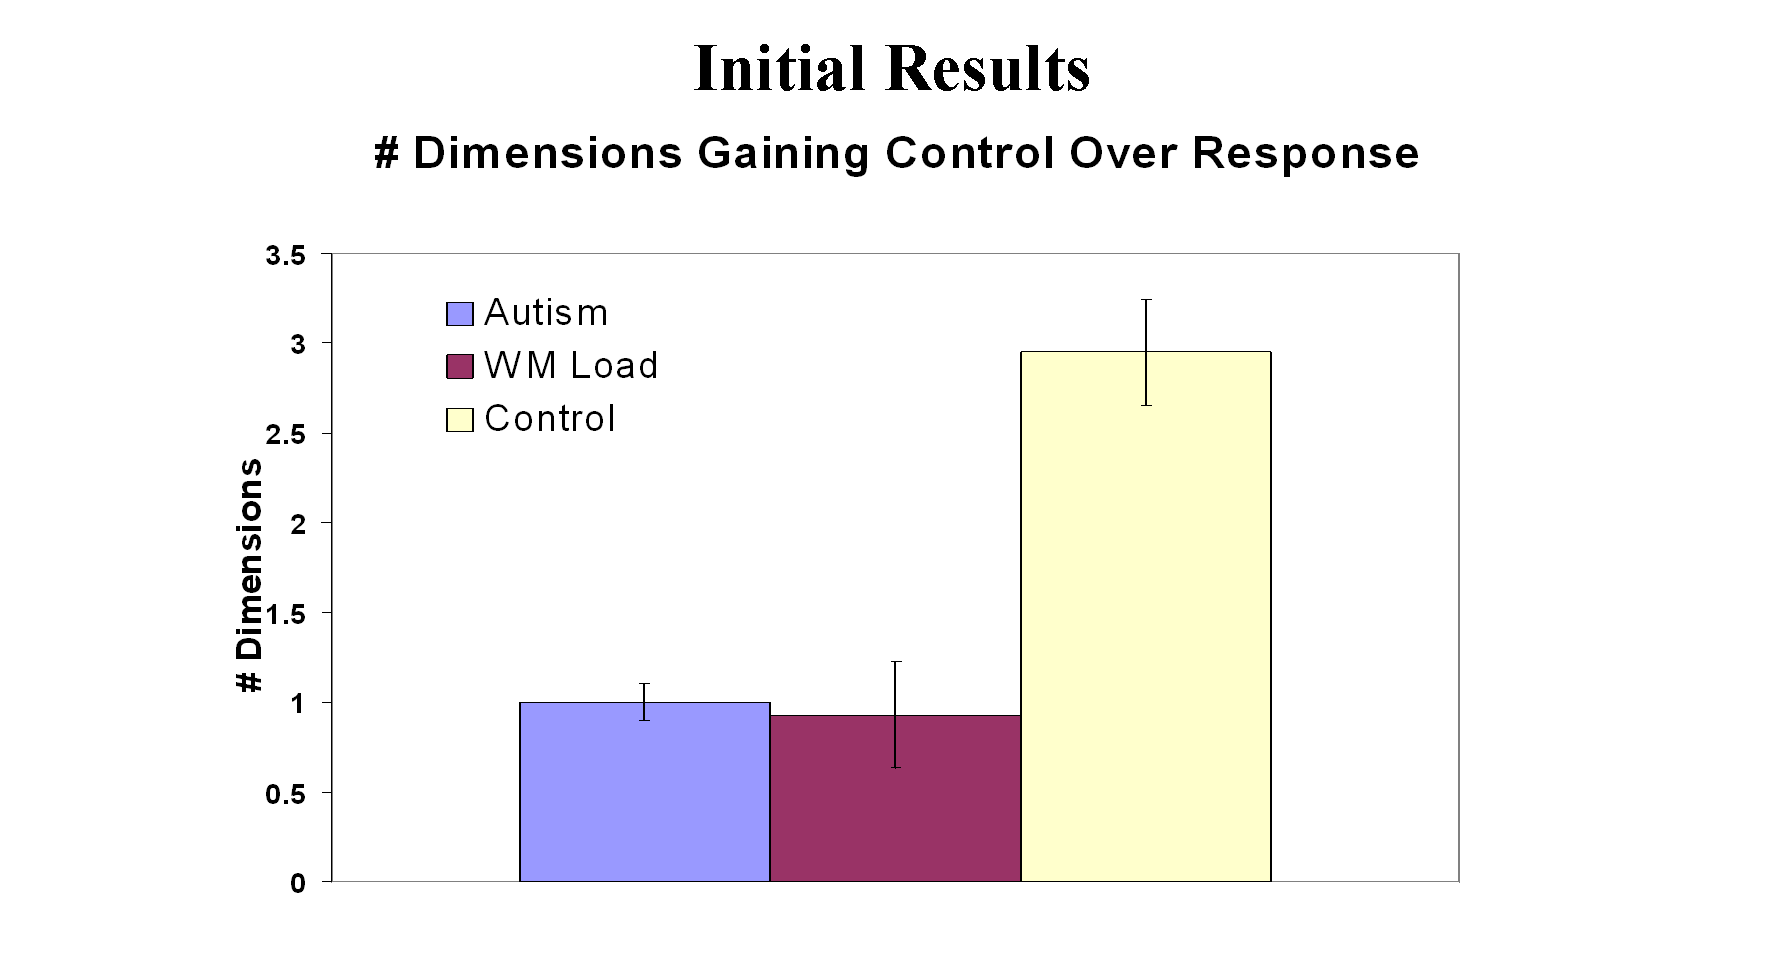
\includegraphics[width=125mm]{graphs/OS_initial_results.eps}
	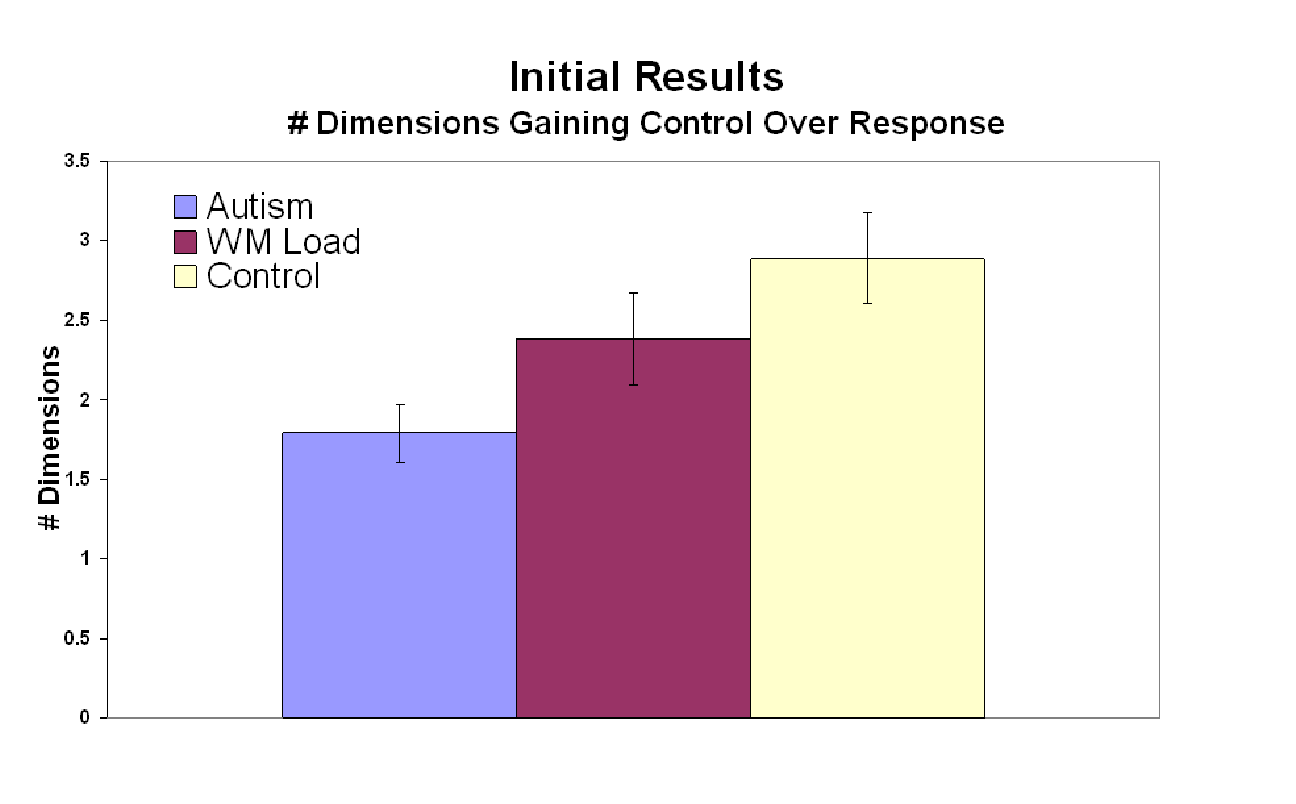
\includegraphics[width=125mm]{graphs/overselectivity_results_new.eps}
\end{center}
\caption{Simulation results modeling overselectivity task (see Figure~\ref{OS-Task}) by manipulating the flexible updating of a PFC-like mechanism. Only the simulation where the PFC is allowed to flexibly adjust the activation of its representations (``normal condition'') resulted in all three components of the compound stimulus gaining equal control over behavior.  Both the inflexible updating (autism condition) and the addition of irrelevant information in PFC manipulations (working memory load condition) result in a restricted subset of components gaining control over behavior, demonstrating overselective behavior.}
\label{OS-Model-Results-2}
\end{figure} 

The model of autistic performance responded to significantly fewer components ($p < .05$), compared to the model allowed to flexibly update its PFC representations, demonstrating overselective behavior.  Providing additional support for the hypothesis that the PFC influences learning in other cortical areas in interesting and important ways, a modeled WM load during training of a ``healthy'' network results in significantly more overselective responding ($p < .05$), also capturing recent behavioral results.  Overselectivity arises in this model due an effect of PFC-directed attention on the learning of associations between stimulus features and the response output.  When PFC activity is directed to a particular stimulus pathway, the activation levels of the hidden units of that pathway are increased.  Lateral inhibition within the Hidden Layer, driven by this increased activity, reduces activity in the pathways corresponding to the other stimulus components.  Thus, learning primarily takes place within the selected pathway, as synaptic plasticity is strongest in Leabra in the presence of presynaptic activity.  In the autism network, which remains focused on a single pathway throughout training, the synaptic weights grow strong only within the selected pathway, with the connections in the other pathways remaining relatively weak.  Thus, the autism network fails to learn to generate responses to the unattended stimulus features, even if attention is later directed to those features.  In contrast, the healthy model flexibly adjusts PFC activity during training, allowing different pathways to be strengthened on different trials, eventually producing strong associations between all of the stimulus features and the need to respond.  Leabra's Hebbian learning mechanism further ensures that these associations are robust. (See Figure~\ref{OS-Model-Cartoon}.)

\begin{figure}
\begin{center}
	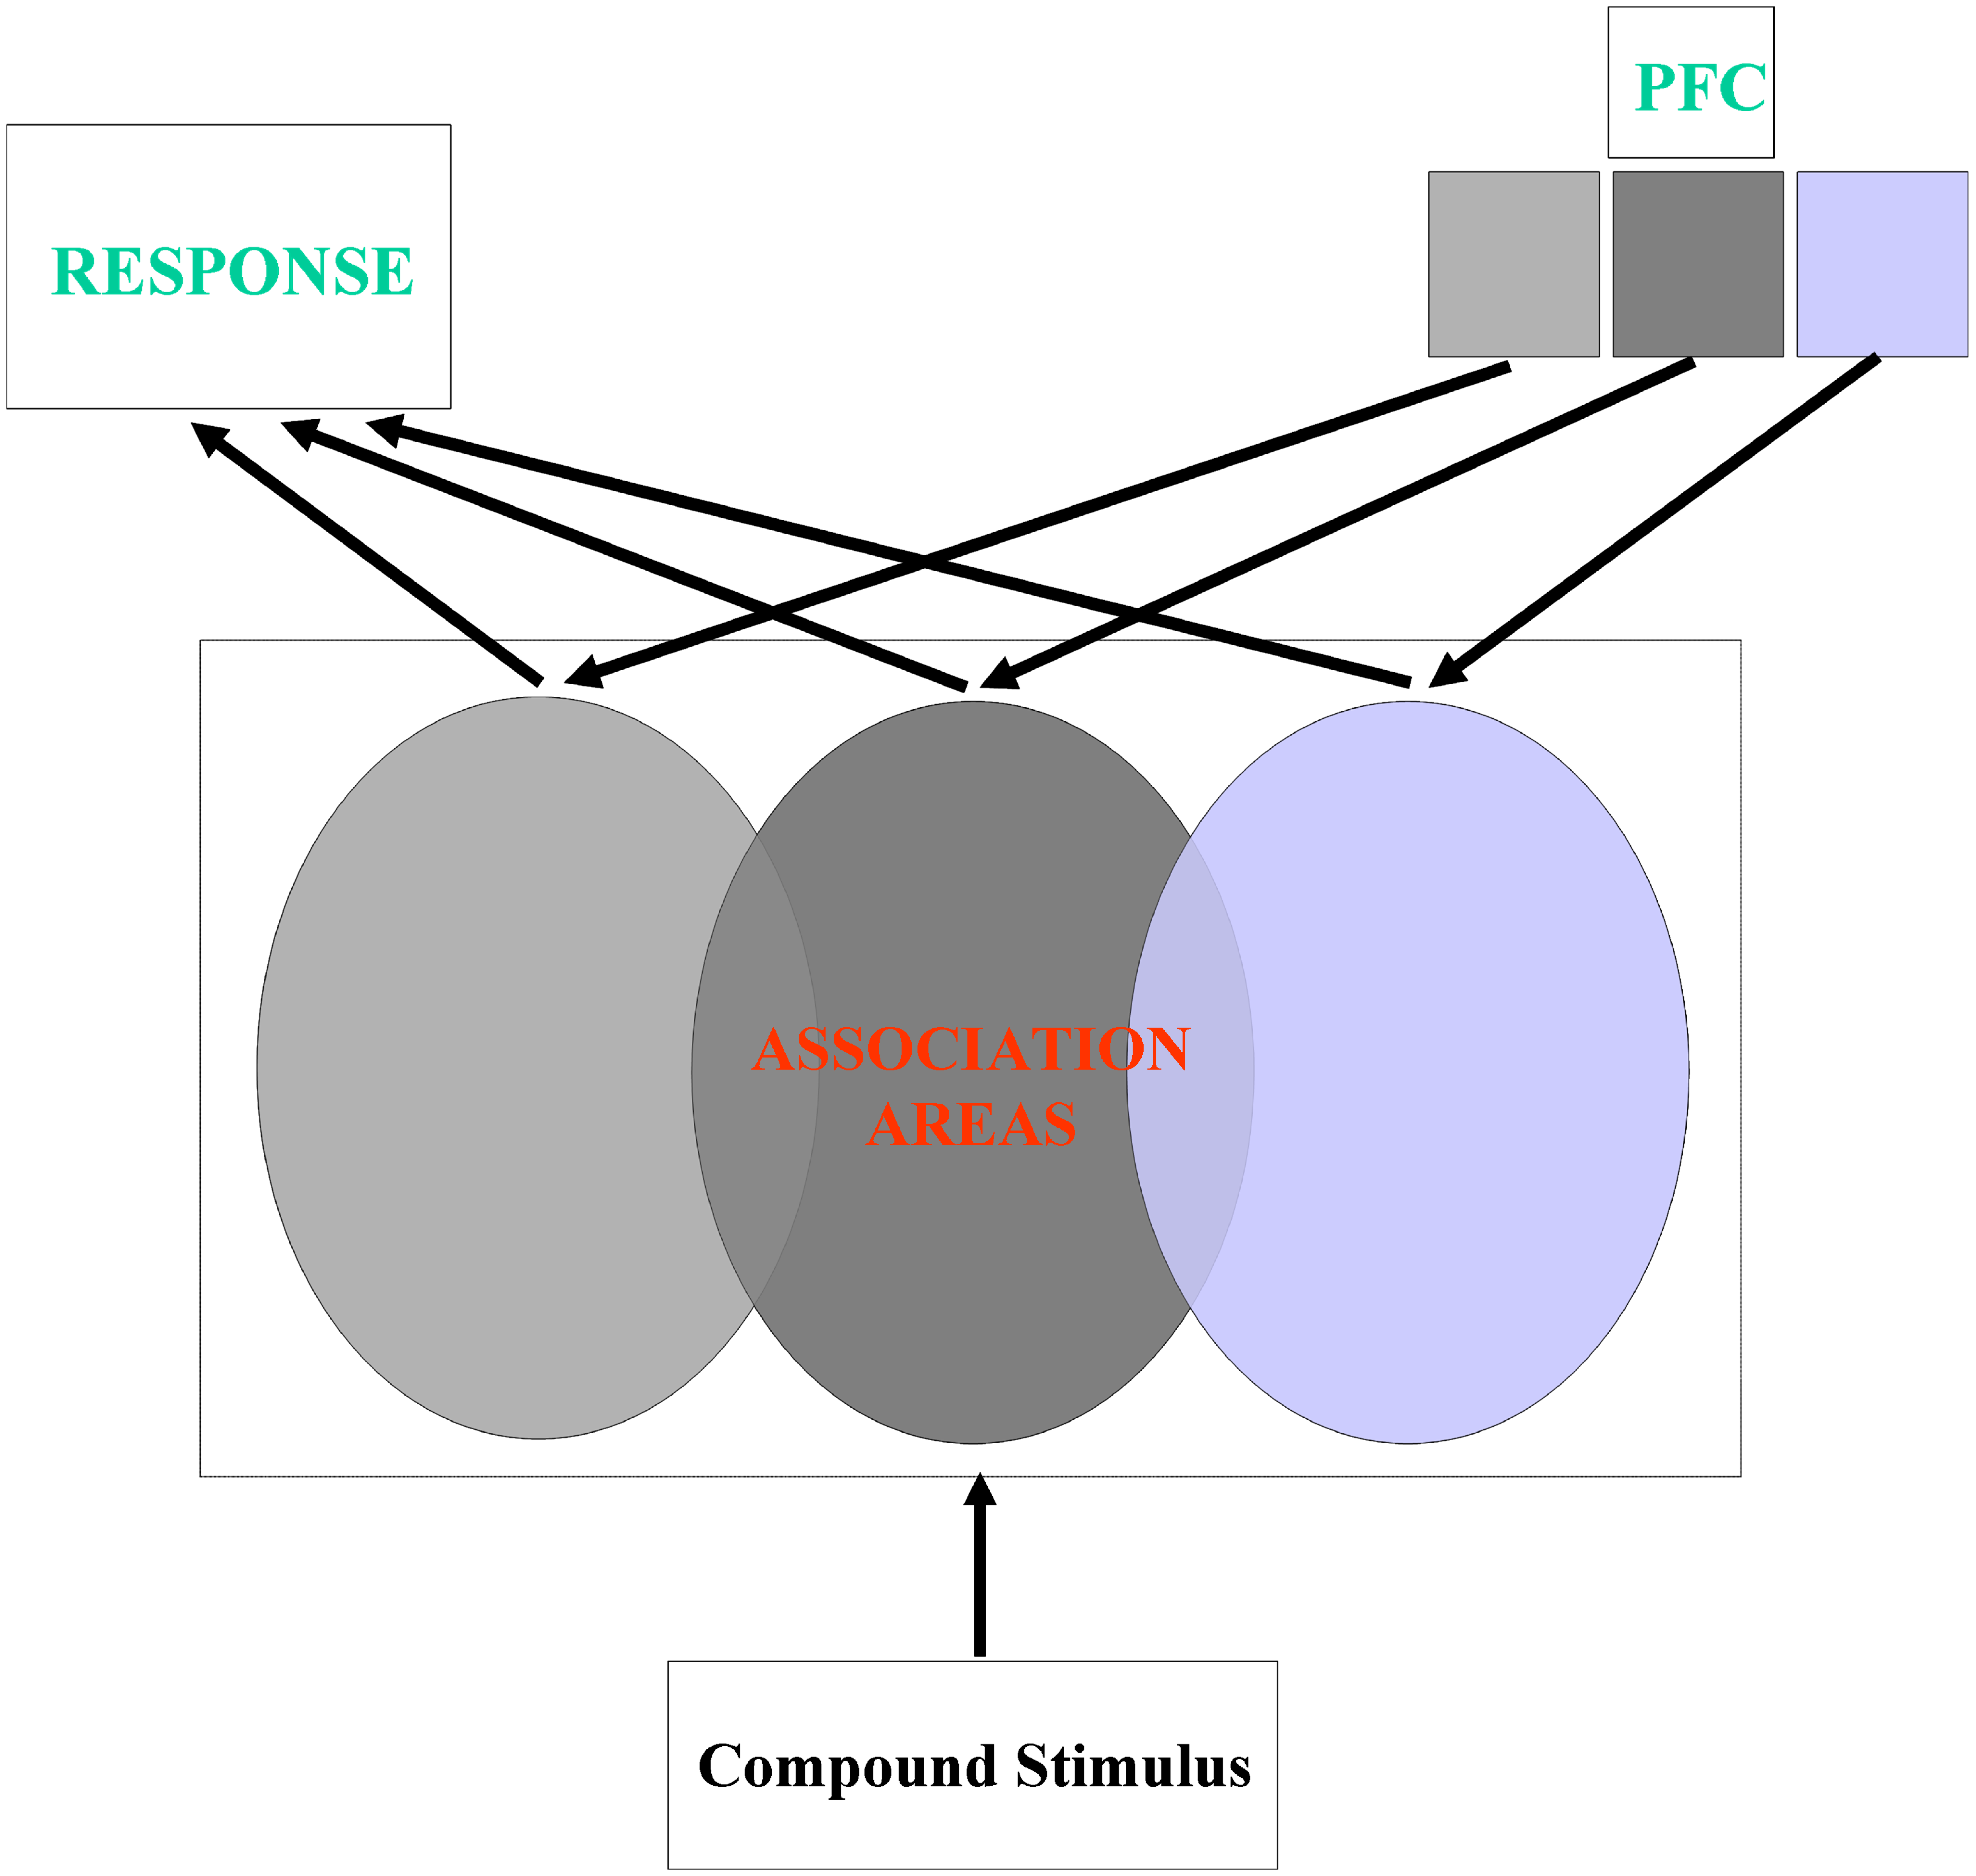
\includegraphics[width=70mm]{figures/so_model_no_persev_new_2.eps}

-----------------------------------------------------------

	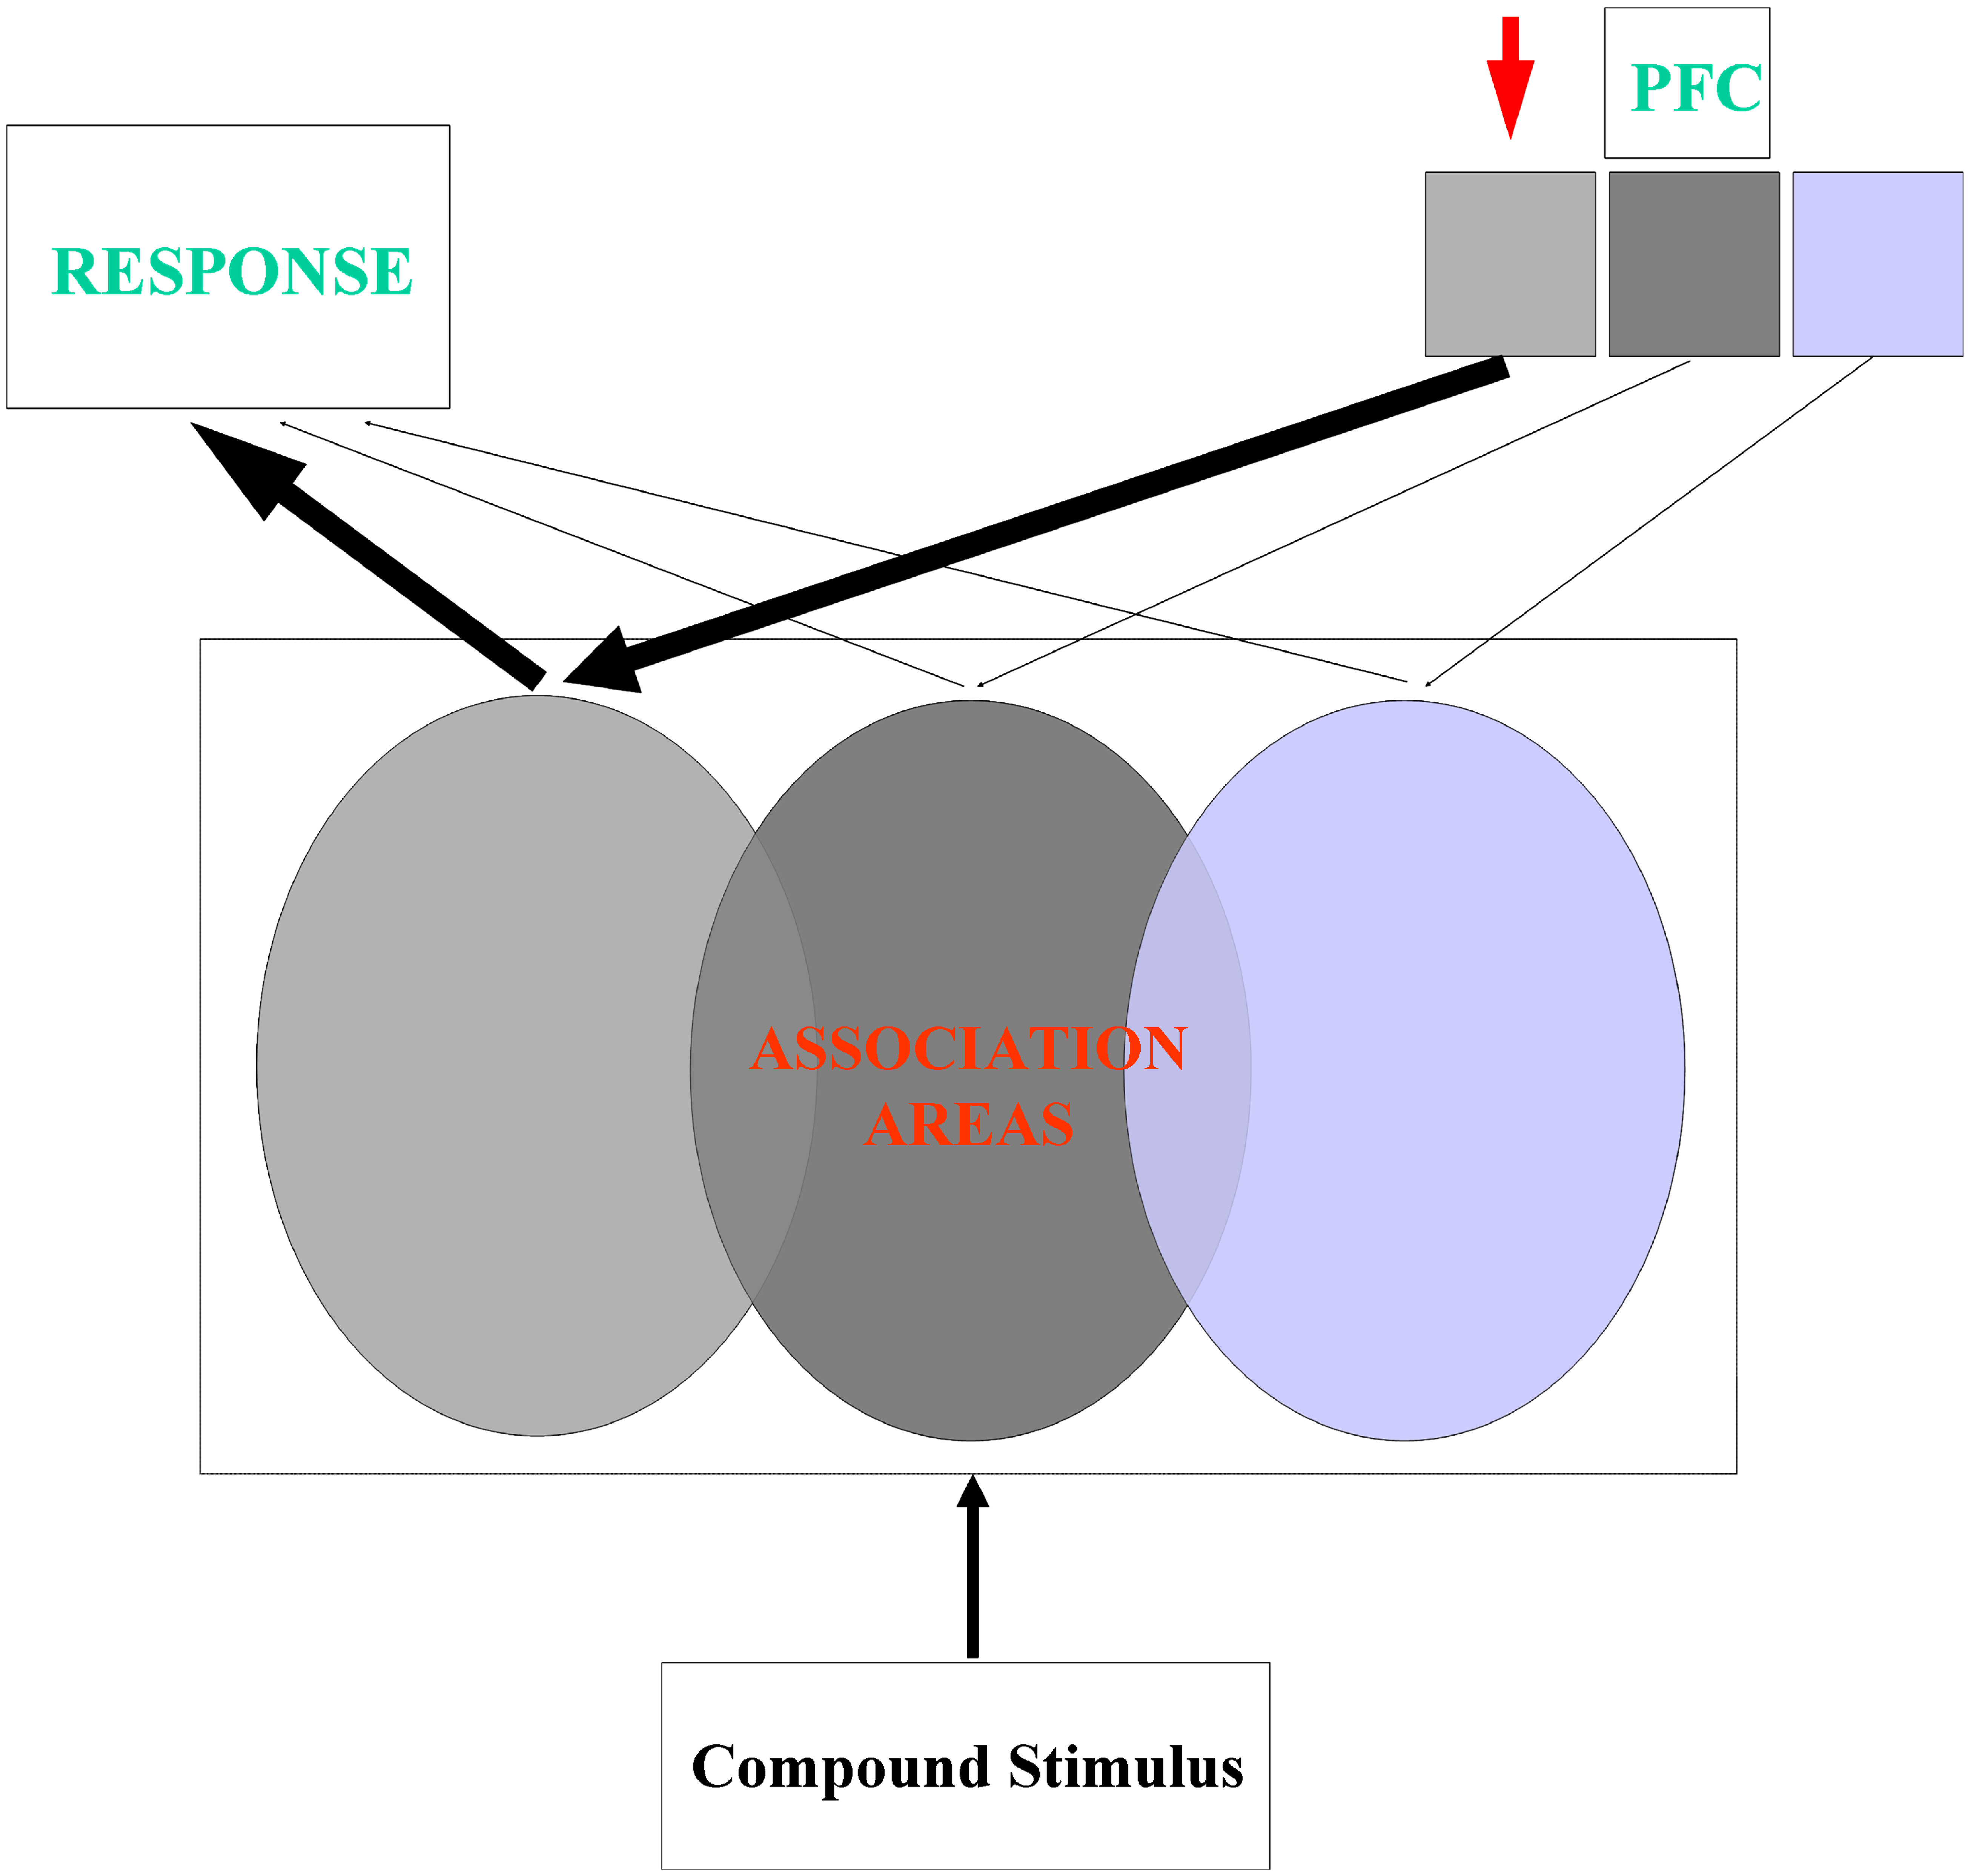
\includegraphics[width=70mm]{figures/so_model_d1_persev_new_2.eps}
\end{center}
\caption{Top panel represents a cartoon model of the stimulus overselectivity task where the PFC is able to flexibly adjust its representations (normal condition).  The resulting ``weights'' driving the response are all similar, resulting in each dimension or feature having equal influence over the response.  The bottom panel represents inflexible updating of the PFC (autism condition).  The red arrow indicates that the PFC is ``stuck'' on the first dimension or feature.  The weights are biased in favor of the feature perseverated on by the PFC, resulting in behavior being dominated by a restricted subset of those available, demonstrating overselectivity when simulating autistic performance.}
\label{OS-Model-Cartoon}
\end{figure} 

%The modeling results presented here suggest that, in people with ASD, overselectivity may be driven largely by a learning process that depends upon the PFC to provide appropriate contextual information in learning stimulus to response mappings.  When the PFC is unable to flexibly and appropriately update its contents, representations in cortical areas downstream from the PFC result which are dominated by an overly restricted, or possibly even irrelevant, subset of features and items from the environment. Results presented here, coupled with past research, provide further support for a theory of perseverative attention to a restricted subset of features in autism.  Indeed, my work provides a plausible mechanism explaining information integration problems in people with ASD.   

\subsection{Summary}
The modeling results presented here suggest that, in people with autism, overselectivity may be driven largely by abnormalities in DA/PFC interactions, causing inflexibility in the shifting of top-down attention.  When the PFC is unable to flexibly and appropriately update its contents, representations in cortical areas downstream from the PFC develop which are dominated by an overly restricted, or possibly even irrelevant, subset of features from the environment.  Poor generalization occurs, under this account, due to the same abnormal cortical representations.  The inability to flexibly update the PFC increases the likelihood that the only environmental associations that will be learned in a given situation will involve spurious correlations (e.g., idiosyncratic features of the training process), with other, more relevant, factors escaping attention.  Subsequent dependence on such spurious correlations can cripple generalization performance.  We suggest that learning over extended developmental timescales with this impairment may lead to behavior which looks like an integration problem on the surface, but, is actually just integrating a limited amount of information.  The results presented here, coupled with the previous research on how DA/PFC impairments can explain executive dysfunction in autism, provide further support for a common neurological cause underlying a variety of behaviors observed in autism.   




\section{Implicit Learning}
\label{section:implicit}

%
% Implicit Learning
%

\subsection{Implicit Learning Deficits in Autism}

%Investigations into implicit learning in autism have led some researchers to suggest a general deficit in this domain.  Poor performance on tasks such as the learning of artificial grammars~\cite{ReberAS:1967:Implicit} and an apparent lack of learning during serial response time tasks (SRTT) have been used in support of this conjecture~\cite{MostofskySH:2000:Procedural,KlingerLG:2006:Implicit}.  A proposed computational exploration of the behavioral data utilizing the SRTT will be completed as part of this research project.  

%In addition to executive dysfunction and stimulus overselectivity, is it plausible that abnormal PFC/DA interactions can also account for the deficits in implicit learning observed in people with autism?  Implicit learning is learning that occurs without any awareness of the specific knowledge acquired during the process.  Researchers have suggested that people with autism have a core deficit in their ability to implicitly learn about the inherent relationships that exist between objects and situations in the world~\cite{MostofskySH:2000:Procedural,KlingerLG:2006:Implicit}.  Klinger et al. argue that impaired implicit learning results in difficulties in recognizing the relationships that exist across experiences, likely leading to problems forming general knowledge about categories of items and types of situations.  Difficulties in generalizing learned knowledge to new situations are commonly observed in people with autism, and these difficulties frequently act as a central obstacle to the development of behaviors needed for autonomy and independent living.  Thus, a precise characterization of the mechanisms responsible for these generalization deficits would be very valuable to any effort to design ways to mitigate these serious issues in people with autism.

Some researchers have suggested that people with autism display a deficit in the implicit learning of relationships that exist between objects and situations in the world~\cite{MostofskySH:2000:Procedural}. Klinger, Klinger, \& Pohlig~(2006) \nocite{KlingerLG:2006:Implicit} argue that impaired implicit learning results in difficulties in recognizing relationships across experiences, leading to problems with acquiring general knowledge. People with autism commonly have difficulties generalizing learned knowledge to new situations, hindering the learning of behaviors needed for independent living.
% Thus, a precise characterization of the mechanisms responsible for these generalization deficits would be very valuable to efforts designed to mitigate these serious issues.

Poor performance when learning artificial grammars~\cite{ReberAS:1967:Implicit} and learning deficits on serial response time tasks (SRTT) have been used as evidence for general implicit learning impairments in ASD~\cite{MostofskySH:2000:Procedural,KlingerLG:2006:Implicit}. In the following, we focus on SRTT phenomena.

\subsection{The Serial Response Time Task (SRTT)}

%In a common version of SRTT, participants are presented with four buttons, with exactly one button illuminated at any one time.  Participants are asked to simply press the currently illuminated button as quickly and accurately as possible.  Once a button is depressed, a new button is illuminated, prompting the participant to press the new button, and this sequence of cued button presses continues for a block of 80 responses, with an experimental session consisting of five of these blocks.  The illumination order of the buttons is the key manipulation of the SRTT.  During the first and the final (fifth) block the order in which the buttons are illuminated is random.  However, during blocks 2, 3, and 4 there is a hidden pattern in the responses that are required.  This hidden structure is apparently detected by many healthy participants, as there is a significant reduction in the reaction time required to press the correct button across blocks 2, 3, and 4.  Importantly, this reduction in reaction time does not occur during the randomized first and fifth blocks.  The common interpretation of these results is that learned knowledge of the hidden sequential pattern allows participants to better ``anticipate'' which button will be illuminated next, allowing them to prepare this upcoming action and, thereby, speed their response.  Knowledge of the hidden structure is seen as ``implicit'', however, as most participants claim no explicit knowledge of the sequential pattern~\cite{CleeremansA:1991:SSRT}.

In a common version of SRTT, participants press buttons, one at a time, as they are illumnated or highlighted. The order of illumination is the key manipulation. During the first and the final (fifth) block of trials, the order in which the buttons are illuminated is random. However, during blocks 2--4 there is a hidden sequential pattern in the buttons that are illuminated. An observed reduction in the reaction time of correct button presses during blocks 2--4 indicates that healthy participants become sensitive to the hidden pattern. Importantly, this reduction is not observed during blocks 1 and 5. Knowledge of the hidden structure is seen as ``implicit'', however, as most participants claim no awareness of the sequential pattern~\cite{CleeremansA:1991:SSRT}. In contrast, people with autism do not show marked improvement during blocks 2--4, suggesting that autism impairs implicit learning abilities~\cite{MostofskySH:2000:Procedural}.

While this behavioral result is interesting in its own right, it also raises questions concerning the biological mechanism(s) behind this deficit. There is some evidence that PFC and the basal ganglia are important for implicit learning~\cite{MatsumotoN:1999:Sequential,PascualLeone:2004:PFCImplicit}. We have explored this connection using an established computational model of the SRTT, investigating the possibility that PFC/DA abnormalities may give rise to the implicit learning problems observed in ASD.

%Some insight might be gained from the neuropsychological literature involving the SRTT.  Specifically, deficits in tasks assessing implicit learning have been linked to damage to the cerebellum.  This is intriguing, as there is ample evidence of cerebellar abnormalities in people with autism~\cite{CourchesneE:1994:CerebellumAttentionShift}.  However, other tasks traditionally associated with the cerebellum, such as judgement of timing, show no differences between people with autism and normally developing controls~\cite{MostofskySH:2000:Procedural}.  Recently, evidence has emerged suggesting that PFC and the basal ganglia may be important players in implicit learning as well~\cite{MatsumotoN:1999:Sequential,PascualLeone:2004:PFCImplicit}.  It is this latter connection that we will pursue, here, using an established computational model of the SRTT to investigate the possibility that PFC/DA abnormalities may give rise to the implicit learning problems observed in people with autism.

\subsection{Modeling SRTT Performance}
Seminal work on modeling healthy SRTT performance has been conducted by \nocite{CleeremansA:1991:SSRT} Cleeremans \& McClelland~(1991). In this work, simulated neural circuits were repeatedly presented with an input encoding the currently illuminated button, and the output of the circuit was read as a prediction of the next button to be illuminated. Importantly, these neural networks included a ``context layer'' of neural units which learned to actively maintain information about the sequence of previous inputs, allowing the model to base its predictions on more than the currently illuminated button. These models were essentially simple recurrent networks (SRNs)~\cite{ElmanJ:1990:SRN} trained to predict the next button to be be pressed. We recreated the Cleeremans \& McClelland SRTT model with one small modification. In order to match available SRTT data for people with autism, we reduced the original implementation's 10 buttons (inputs and outputs) to 4 buttons. The schematic network architecture is shown in Figure~\ref{network-diagram-srtt}.  

The Cleermans \& McClelland model assumed that button press reaction times are linearly reduced with button prediction accuracy. Network outputs were converted into a probability distribution over the buttons using a Luce choice ratio~\cite{LuceRD:1963:Ratio}, and the difference between this distribution and the actual next illuminated button was linearly scaled to produce a simulated response time. We used exactly the same method to simulate reaction times, introducing three free parameters: a scaling constant from prediction error to milliseconds, a base response time (when error is zero) for our healthy model, and a base response time for our autism model.
%Note that different base response times were used for the normally developing and autism cases in order to capture the difficulty people with autism regularly exhibit when initiating movements~\cite{RinehartNJ:2001:AutismMovement}.

%\begin{figure}[t]
%\begin{center}
%	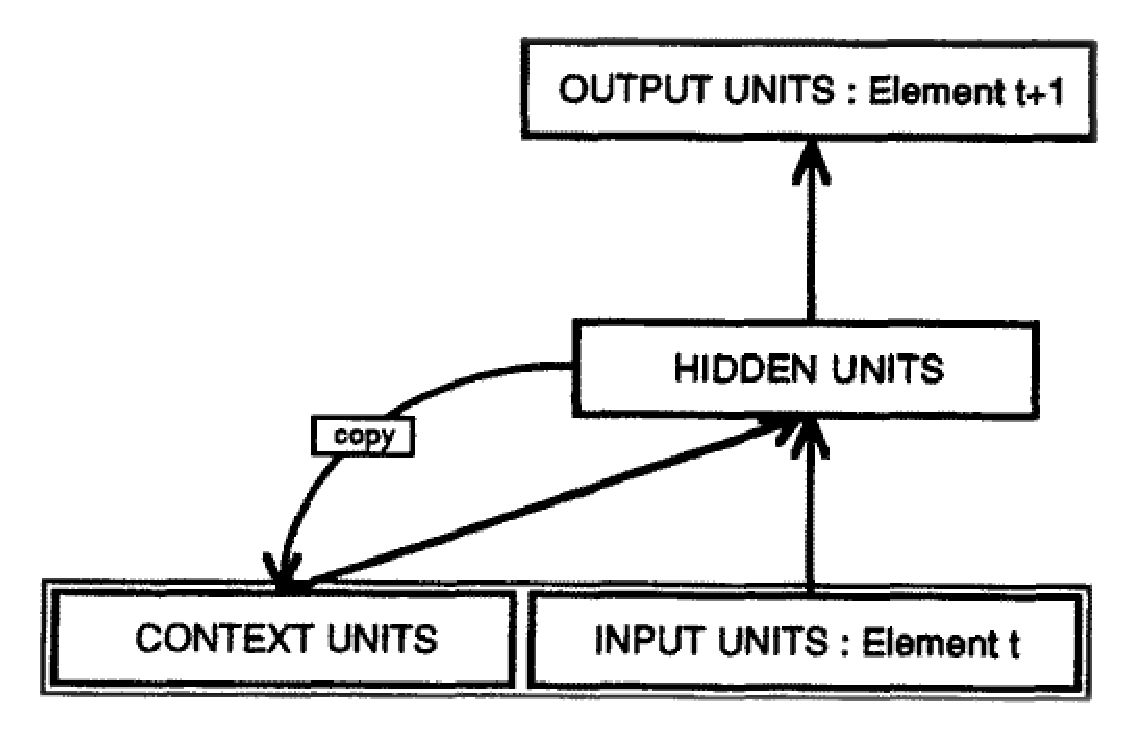
\includegraphics[width=85mm]{figures/srn.eps}
%\end{center}
%\caption{General structure of a Simple Recurrent Network (SRN) model.  Image adapted from Cleeremans and McClelland (1991).}
%\label{SRN-Model}
%\end{figure} 

\begin{figure}[t]
\begin{center}
	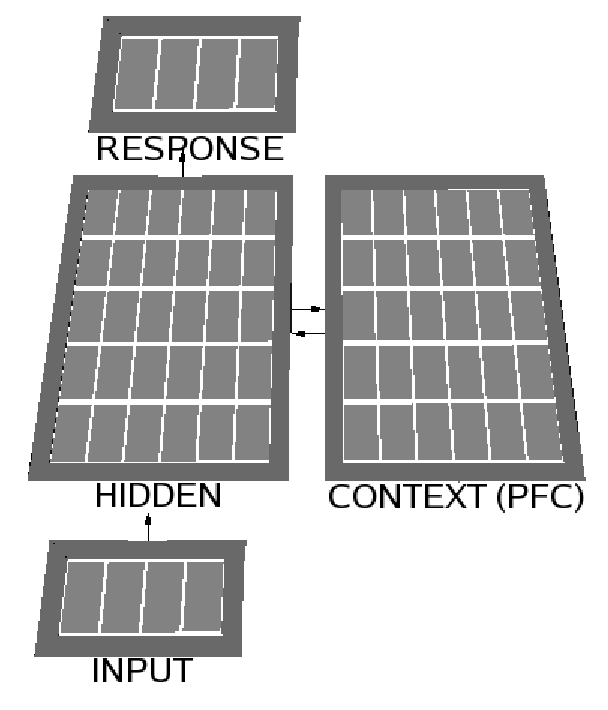
\includegraphics[width=75mm]{figures/srtt_network.eps}
\end{center}
\caption{Network Diagram of SRTT Model} 
\label{network-diagram-srtt}
\end{figure}

% Since the hidden sequential structure in the intermediate blocks of the SRTT is often complex, the information provided by the context layer is vital for the success of the model.  Importantly,
The context layer in the Cleeremans \& McClelland model played an identical functional role to the PFC in other models, actively maintaining information to modulate an input-output mapping. In this case, the context layer actively maintained information about the preceding button presses, influencing the prediction of the next button. In our executive dysfunction model, described previously, the PFC was updated in a dynamic fashion, based on learned task contingencies. In this SRTT model, the context layer is updated with each new input. Thus, the SRN context layer is analogous to the PFC in XT, with the updating ``gate'' forced to open with each new input~\cite{OReillyRC:2000:Computational}.
%~\cite{OReillyRC:2006:MWMW}.
%Since the hidden sequential structure in the intermediate blocks of the SRTT is often complex, the information provided by the context layer is vital for the success of the model.  Importantly, the context layer in this model plays an identical functional role to the PFC in other models, actively maintaining information that can be used to modulate an input-output mapping.  In our previous executive dysfunction model, the PFC actively maintained information about the currently relevant stimulus dimension (e.g., ``focus on the ink color'' in Stroop or ``sort cards based on shape'' in WCST), so as to modulate performance.  In this model, the context layer actively maintains information about the preceding button presses, allowing that information to modulate the prediction of the next button.  In our previous model, the PFC was updated in a dynamic fashion, based on learned task contingencies.  In this model, the context layer is updated with each new input presentation.  Thus, the SRN context layer is analogous to the PFC in our previous model, with the updating ``gate'' forced to open with each new input~\cite{OReillyRC:2006:MWMW}.

In order to capture the relevant sequential information, the SRN model must update the context layer in a fast and appropriate manner. This flexible updating of contextual information is precisely the cognitive mechanism we hypothesize to be suspect in people with autism. By restricting the ability of the SRN to update the context layer, mirroring the PFC updating failures that arise with weakened PFC/DA interactions in our other models, we aimed to capture the performance of people with autism. We implemented this updating restriction with a single new parameter: a probability that context layer (PFC) updating will be successful with each new input. Healthy behavior was modeled by setting this probability to one, and the probability was reduced to model ASD performance. This manipulation is analogous to reducing the efficacy of the DA-based gating signal to the PFC.  Restricting the updating of the PFC, in this manner, makes the temporally extended information stored there much less reliable, hindering the learning of complex sequential structures in the ASD model.


\subsection{Implicit Learning Simulation Results}
Model simulations were repeated $100$ times in each of the experimental conditions, with initial synaptic connection strengths randomized for each repetition. Average performance results for each block were compared to previously reported response time data for both people with autism and typically developing controls~\cite{MostofskySH:2000:Procedural}. The context layer updating probability and the response time scaling parameters that produced the lowest sum-squared deviation from the human data were identified as the best fit model.

The resulting modeled reaction times, along with previously reported human data, appear in Figure~\ref{Model-Results}. The best-fit updating probability for the autism model was found to be $0.5$. A repeated measures ANOVA on blocks 1, 2, 3, and 4 of the model results showed a significant Group by Block interaction ($p < 0.000001$). This indicates that the ASD networks demonstrated significantly less learning over the crucial training blocks (2--4) than the networks allowed to reliably update their PFC-like context layers. Thus, clear implicit learning deficits were found in the autism model.

%The simulation results match human performance both qualitatively and quantitatively, providing evidence that impairments in PFC updating can result in implicit learning deficits like those seen in people with autism.  When the healthy network is restricted to perfectly update its Context Layer (i.e., with probability one), the corresponding best-fit probability for the autism network is $0.5$, with an SSE of $652$. The corresponding scaling parameter from error to reaction time is $261.4$, the healthy base time is $458.6$ msec, and the autism base time is $534.5$ msec.  The resulting modeled reaction times, along with human data from the literature, is shown in Figure~\ref{Model-Results}.

\begin{figure}[t]
\begin{center}
%%	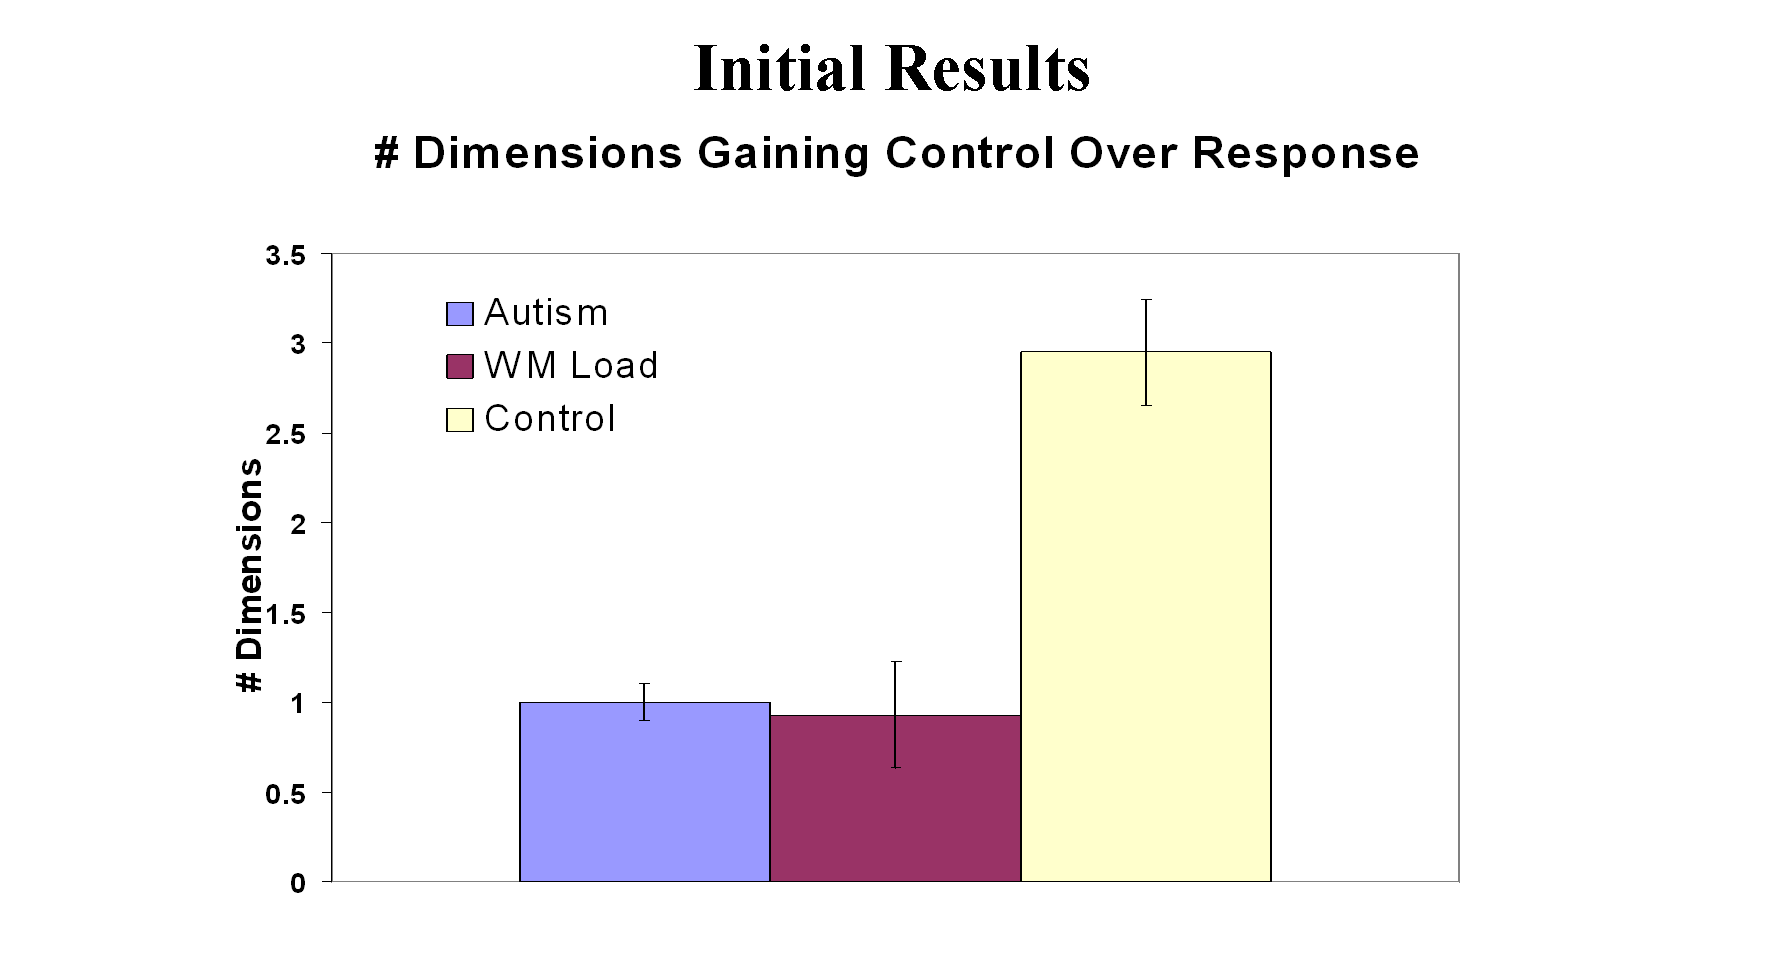
\includegraphics[width=125mm]{graphs/OS_initial_results.eps}
	\includegraphics[width=75mm]{graphs/srtt_chart.ps}
\end{center}
\caption{Model Results \& Human Behavioral Data from Mostofsky
         et al. (2000)} 
\label{Model-Results}
\end{figure} 

\subsection{Summary}

Our simulation results matched human performance both qualitatively and quantitatively, providing evidence that impairments in PFC updating can result in SRTT deficits like those seen in ASD. It is interesting to note that this account posits deficits in learning temporal patterns rather than in implicit learning, per se. More information about these simulations may be found in Kriete \& Noelle~(2009).\nocite{KrieteT:2009:SRTT}

%The modeling results presented in this section suggest that, in people with autism, implicit learning deficits may be driven largely by abnormalities in DA/PFC interactions, causing inflexibility in the updating of contextual information.  Without the proper updating of actively maintained contextual information, it is essentially impossible to properly integrate temporally separated pieces of information, such as the order of items in a sequence.  Thus, our computational account highlights how PFC/DA dysfunction can lead to problems with information integration.  This is particularly interesting, since one prominent behavioral theory of autism, \emph{Weak Central Coherence}, posits that deficits in integrating contextual information lay at the core of this disorder~\cite{HappeF:1999:WCC}.  



\section{Lexical Disambiguation}
\label{section:lexical}

%
% Lexical Disambiguation
%

\subsection{Using Sentential Context}
We have presented examples of how inflexible attentional modulation of posterior brain areas by the PFC, caused by deficient DA / PFC interactions, can account for an increasingly diverse set of behaviors including executive dysfunction and implicit learning differences in people with ASD.  In the previous section on implicit learning in autism, we showed how this deficit can lead to problems integrating information over temporally extended time frames.  Another situation that requires the integration of information across experiences is our ability to understand the meaning of ambiguous words in a sentence.  Homographs are words with one spelling, but different pronunciations and meanings, such as ``bow'' and ``tear''.  In order to determine the proper pronunciation (and meaning) of a homograph, we must rely on the sentential context. People with autism appear unable to properly utilize this context in order to correctly pronounce homographs.  Instead, they will rely on the statistically most frequent pronunciation~\cite{RefWorks:103,HappeF:1997:WCC_Homographs}.  
Contemporary connectionist models of sentence processing utilize an SRN which possess a ``context layer''.  The context layer provides a means to integrate past information, such as the previous words read, into an evolving representation of a sentence.  The information provided by the context layer is vital for the success of the model on tasks such as homograph pronunciation.  As before, the SRN must update the context layer in a fast and appropriate manner in order to provide the appropriate contextual information.  

\subsection{Lexical Ambiguity in Schizophrenia}
A possible clinical comparison group for lexical disambiguation performance in people with autism can be found in people with schizophrenia.  It is known that schizophrenics demonstrate problems utilizing context across a number of tasks, including language disambiguation tasks~\cite{CohenJD:1992:Schizophrenia}.  This is a very interesting comparison for a two reasons:

1.  While people with schizophrenia demonstrably possess problems utilizing context when disambiguating words in natural language processing, the specific pattern of deficits is qualitatively different than the same behavior observed in people with autism, as discussed in more detail below.

2.  Many of the symptoms of schizophrenia are believed to arise due to abnormal dopamine functioning~\cite{CohenJD:1992:Schizophrenia}.  

If schizophrenia is believed to have similar underlying deficits to autism, namely a dopamine abnormality, how can the two disorders produce qualitatively different deficits on this psychological task?  The answer lies in the details of the \emph{kind} of dopamine deficit that is posited by theorists in both disorders.  Dopamine is believed to have at least two different kinds of effects on cortical processing.  The first, known as ``tonic'', is believed to enact its effects over a relatively long time scale.  The second, known as ``phasic'', is argued to have rapid influence on cortical processing.  According to Cohen and Servan-Schreiber (1992), abnormal dopamine functioning in schizophrenia is associated with the slower effects of tonic DA.  However, the precise firing and timing of the mesolimbic dopamine cells that inspire the TD-Learning based account upon which our theory is based, are of the second type, phasic dopamine.  In the following we explore, computationally, how the inability to properly update the PFC can explain the psychological profile of people with autism on lexical disambiguation tasks, as well as how different kinds of DA processing may result in the qualitatively different, but still deficient, behavioral profiles of schizophrenia and autism. 

\subsection{Differences Disambiguating Context in Schizophrenia and ASD}
The same general psychological test has been used to test people with schizophrenia and ASD on their ability to utilize context when disambiguating the meaning of words~\cite{CohenJD:1992:Schizophrenia,RefWorks:103,HappeF:1997:WCC_Homographs}, the disambiguation of homongraphs. The ambiguous homographs have two different interpretations, one is the most common or high frequency interpretation, and the other is the least common, or low frequency version.  In this task, a sentence fragment is presented which contains one ambiguous word (e.g. ``without a PEN'') along with a sentence fragment which can disambiguate the meaning of the ambiguous word (e.g. ``You can't keep your chickens'').  The sentence fragments are created to enable the contextually relevant information to be presented before or after the ambiguous word.

The sentences are distributed across four conditions.  (1)  The low-frequency meaning is correct and the context comes last. (2)  The low-frequency meaning is correct and the context comes first.  (3)  The high-frequency meaning is correct and the context comes first (4) The high-frequency meaning is correct and the context comes last.

People with autism demonstrate problems utilizing context in both conditions (1) and (2), providing a significantly higher percentage of incorrect high-frequency responses compared with normally developing control groups~\cite{RefWorks:103,HappeF:1997:WCC_Homographs}.  (See Figure~\ref{asd-lexamb-study}.)  The autism group was not significantly different than controls on conditions (3) and (4), showing no obvious bias in determining the meaning of high-frequency words.  The profile for schizophrenics is slightly different.  People with schizophrenia do show an impairment in utilizing context, but only during condition (2), when the context is presented first. (See Figure~\ref{schiz-lexamb-study}.)  Theorists have interpreted this result as evidence for problems using temporally extended context in schizophrenia.  Condition (4) was not tested in the schizophrenic population, and therefore no human data is available.  
%To clarify, this suggests that in condition (1), the contextual information was temporally close enough to the required response to enable the subjects diagnosed with schizophrenia to correctly utilize this information and make a proper response.  Condition (4) was not tested in the schizophrenic population, and therefore no human data is available.  

\begin{figure}[tp]
\begin{center}
	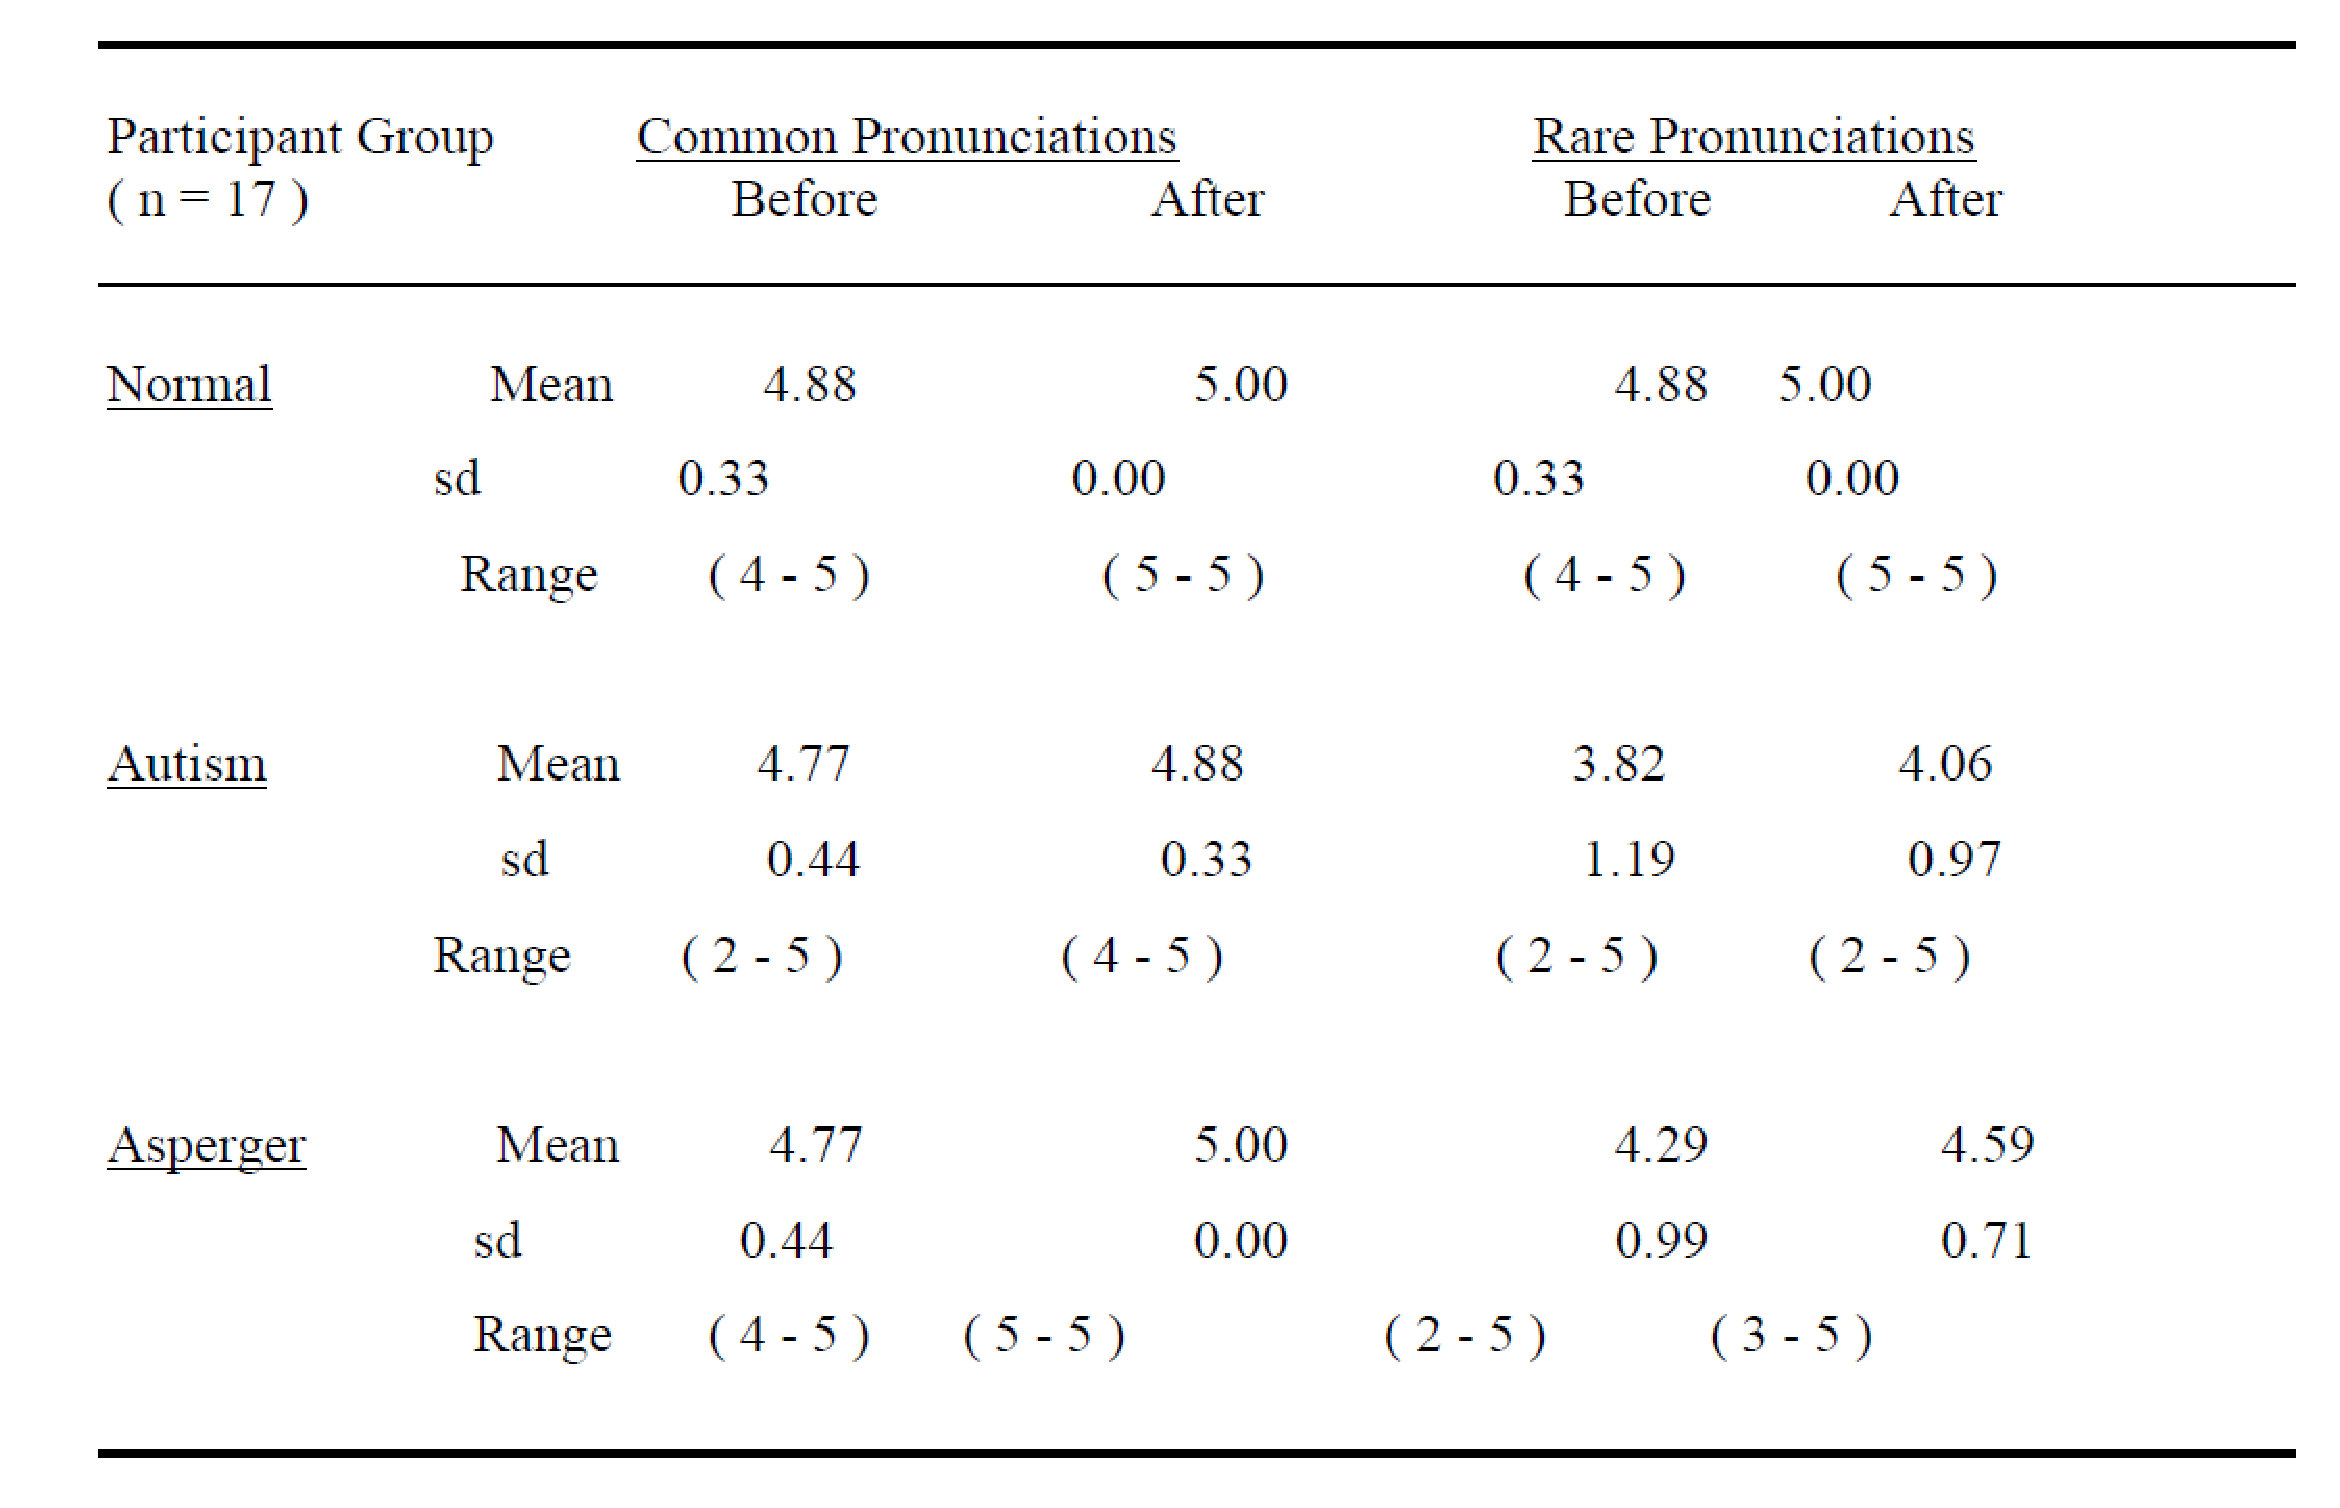
\includegraphics[width=115mm]{figures/asd_lexamb_study_results.eps}
\end{center}
\caption{Results from study on lexical disambiguation in people with ASD.  Common Before/After refers to a common interpretation of the homograph, and it occurring Before/After the contextual information respectively.  Similarly, Rare Before/After refers to a rare interpretation of the homograph, and it occurring Before/After the contextual information respectively.  Table from Jolliffe and Cohen (1999).}
\label{asd-lexamb-study}
\end{figure} 

\begin{figure}[tp]
\begin{center}
	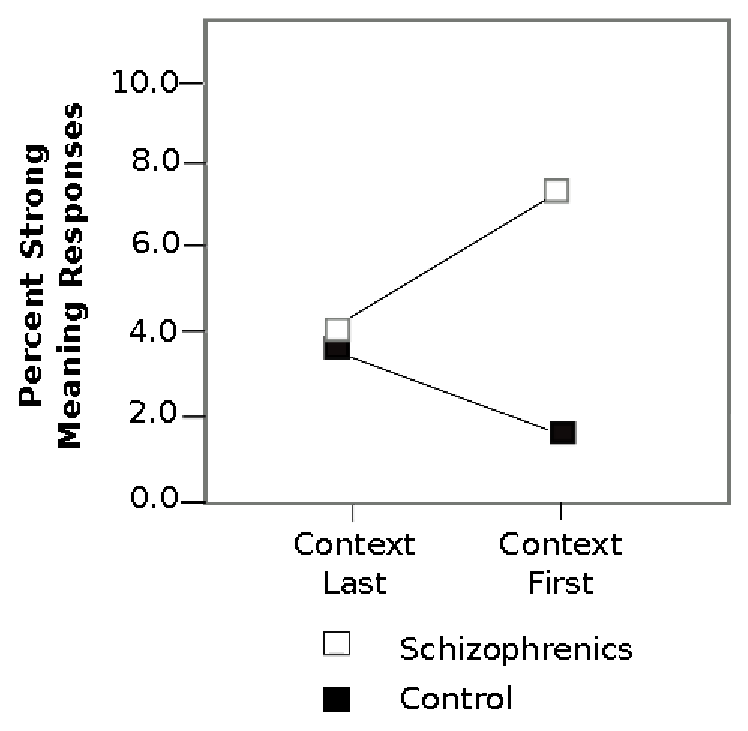
\includegraphics[width=100mm]{figures/schiz_lexamb_study_results.eps}
\end{center}
\caption{Results from study on lexical disambiguation in people with Schizophrenia.  Y-axis shows percentage of errors using the most common interpretation of the homograph, when the rare interpretation was correct.  Figure adapted from Cohen and Servan-Schreiber (1992).}
\label{schiz-lexamb-study}
\end{figure} 

\subsection{Modeling Lexical Disambiguation Effects in Autism}

\subsubsection{A Model of Word Sense Disambiguation}
The connectionist model utilized in Cohen and Servan-Schreiber (1992) was modified to investigate lexical disambiguity in people with autism and schizophrenia. (See Figure~\ref{cohen-servan-schreiber-model}.)  A localist code is used to represent words as inputs to the network.  The input layer also contains words that are used as the contextual cues to assist the network in the disambiguation task.  The output of the network (the ``Meaning Output Module'' in Figure~\ref{cohen-servan-schreiber-model}), also uses a localist code to represent the various possible meanings of the network.  Specifically, one unit is used to represent the interpretation of the word ``BANK'' as a ``financial Institution'', and one unit for the alternative meaning ``area next to a river'', etc.  The context layer (labeled ``Discourse Module'' in Figure~\ref{cohen-servan-schreiber-model}), was modified from its original version.  The original ``Discourse Module'' uses hand coded representations to encode sentential context information, meaning the very important process of learning representations which facilitate the integration of previous experience is hard wired.  we replaced the original ``Discourse Module'' version with a SRN layer, allowing the network to learn how to integrate temporally extended information through repeated experience. (See Figure~\ref{lexamb-model-task}.) 

\begin{figure}[tp]
\begin{center}
	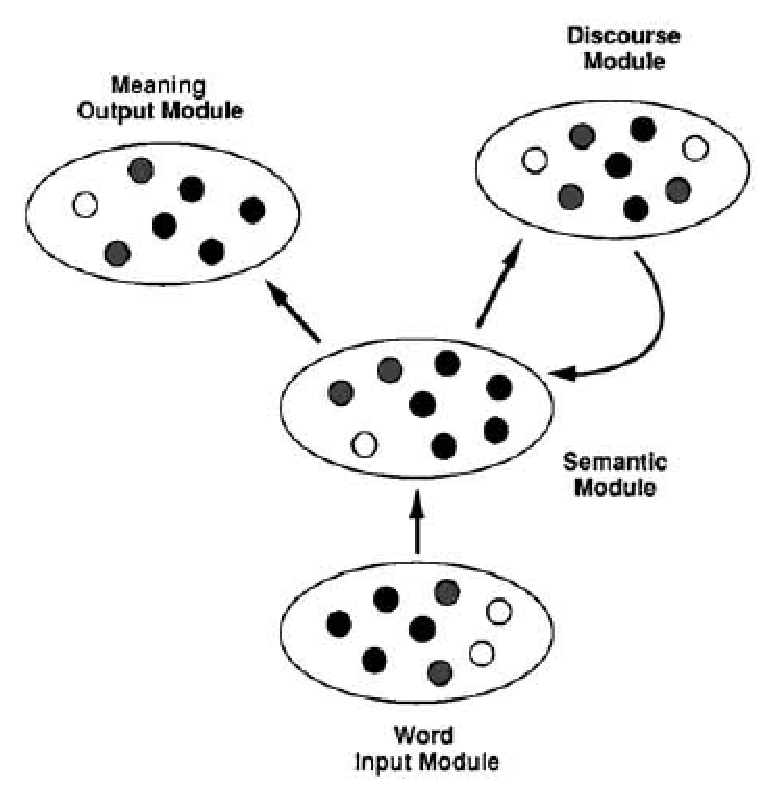
\includegraphics[width=100mm]{figures/Cohen_ServanSchreiber_Model.eps}
\end{center}
\caption{The original lexical ambiguity model. Image adapted from Cohen and Servan-Schreiber (1992).}
\label{cohen-servan-schreiber-model}
\end{figure} 

\subsubsection{Training}
The corpus used for training involved 50 input units representing 50 ambiguous homographs.  Also used as input to the network was 50 disambiguating context units.  Two context units were assigned to each of the 50 homograph units, resulting in each homograph unit being paired with two different context units. Also, each context unit is paired with two different homograph units, ensuring that every context unit is involved in two completely different disambiguation trials.  Setting up the input corpus in this manner prevents the network from learning a one-to-one association of a context unit to a specific homograph word meaning, removing any possibility that the network could solve the task while ignoring all of the homograph units, instead relying only on the information provided by the contextual units to disambiguate the meaning of a homograph.  One context unit was used for the more frequent use (strong) and one unit for the less frequent (weak) use of each homograph.  This will results in 150 possible outputs for the network (100 possible homograph interpretations and 50 context words used for disambiguation of the homographs).  Each possible output can be thought of as representing the proper ``meaning'' input words presented to the network.  (See Figure~\ref{lexamb-model-task}.)  %The network also used 100 units each within the Hidden layer and the Context Layer, it should be noted, however, that varying this value had little effect on the networks overall performance.

One word (input unit) is presented to the network at a time, requiring the network to make a response to every word independent of whether the input is supplied via a contextual or homograph unit.  On each trial, the network is presented with a mini-clause consisting of three words, including a context/homograph pair followed by a homograph probe. The pieces of each mini-clause should be thought of as representing the sentences presented to the subjects in the original study (the context and homograph units), followed by questioning the subjects on the meaning of the ambiguous word (the probe homograph unit).  The order of presentation for the context and homograph units were counterbalanced across all trials, ensuring equal experience with utilizing context at both the beginning and the end of mini-clauses.  The final probe homograph unit was always presented last, and was needed to assess if the network could properly disambiguate the meaning of the homograph after reading the mini-clause.  The network was trained to respond with the correct ``meaning'' for both input types, homograph and context units, by activating a single unit within the output layer which represents the proper semantic interpretation of the input word presented to the network. (See Figure~\ref{lexamb-model-task}.) The network was presented with the strong interpretation of the homographs on 70\% of the trials and the weak interpretation on 30\%.

\subsubsection{Testing}
The same testing procedures as Cohen and Servan-Schreiber (1992) were utilized.  The model was presented with a context and ambiguous word unit pair, one unit at a time.  The order of presentation was again counterbalanced across all testing trials.  After the presentation of the pair, the model was presented with the probe ambiguous homograph word unit.  Note that these are the same ``mini-clauses'' that were utilized throughout the training procedure. The main measure of interest is percentage of incorrect uses of the strong interpretation by the model during the presentation of the probe homograph unit, when the weak interpretation is correct based on the context provided in the mini-clause.  The results were separated into two groups, ``Context Presented First'' and ``Context Presented Last'' to enable comparison to the human subjects data.

\begin{figure}[tp]
\begin{center}
	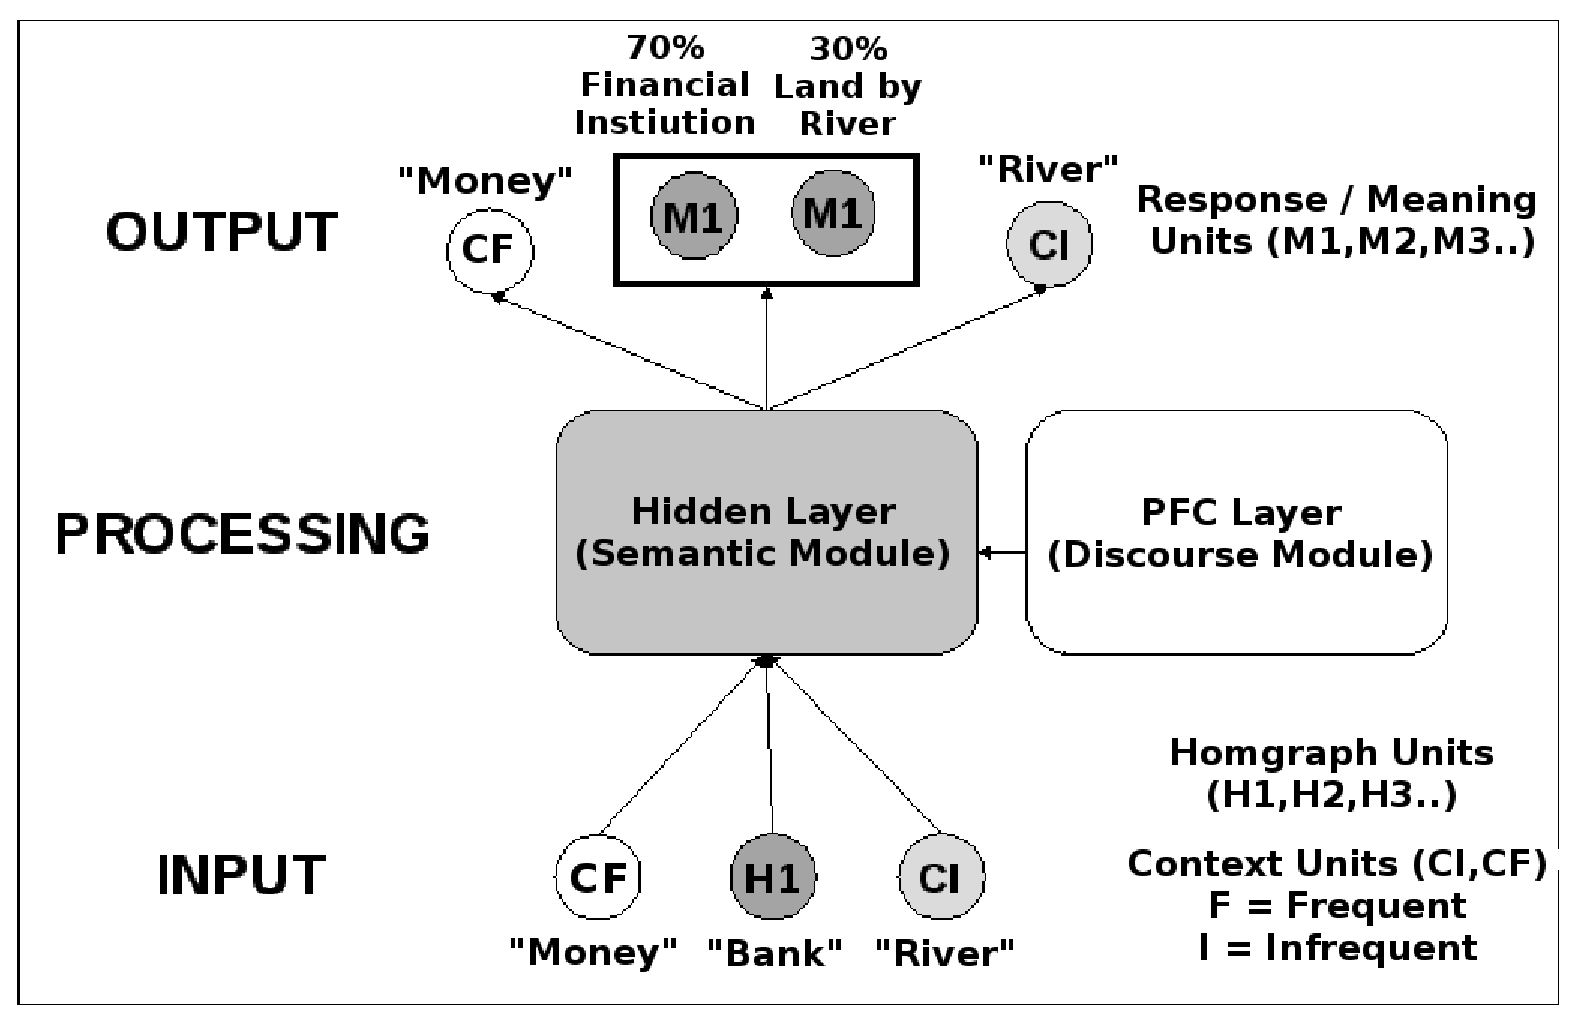
\includegraphics[width=115mm]{figures/lexAmb_network_cartoon.eps}
\end{center}
\caption{Cartoon of the lexical ambiguity model and task.  The task of the model is to correctly respond to any input word presented within the ``INPUT'' layer of the network by activating the unit representing the appropriate meaning at the ``OUTPUT'' layer of the network.  The context units are used to disambiguate the meaning of a specific homograph unit.  Words are presented to the network one at a time and it is the networks job to learn, through experience, to respond with the correct meaning via the ``OUTPUT'' layer of the network.}
%For instance, in this figure the ambiguous homograph input unit represents the word ``Bank'' and the frequent and infrequent context input units represent ``Money'' and ``River'' respectively.  When the infrequent context unit ``River'' is presented first to the network followed by the homograph unit for ``Bank'', the network was expected to learn to use the context unit's meaning to correctly respond ``Land by River''.  This response occurs during the final trial when the network is probed for the correct meaning of the ambiguous homograph unit after the initial mini-clause has been presented.}

\label{lexamb-model-task}
\end{figure} 

\subsubsection{Modeling Schizophrenia}
%We employed the same mechanism used by Cohen and Servan-Schreiber to model the effects of different levels of tonic dopamine on neural processing.  Namely, lowering the gain parameter on modeled neurons within the context layer of the model after initial training has taken place.   Figure~\ref{gain-manipulation} shows the overall effect of this manipulation.  As the gain parameter is increased, the overall effect of the input is heightened.  As the gain decreases, on the other hand, the effect of the net input decreases.  This is believed to mimic the potentiating effects of dopamine on target neurons.  
In the original model of schizophrenic performance of Cohen \& Servan-Schreiber, a hypothesized tonic DA deficit was instantiated by reducing the gain of the activation function on all modeled PFC units. Figure~\ref{gain-manipulation} shows the overall effect of this manipulation.  Coupled with the dynamics of the network, the result was a less stable PFC representation of the contextual information.  Thus, if the context were to come at a point temporally distant from homograph ``probe'', the contextual information maintained within the modeled PFC was more likely to degrade and be of little use to the network.  However, if the context was presented temporally close to the``probe'', the contextual information maintained within the PFC could still be used to disambiguate the meaning.  This manipulation successfully matched the pattern of behavior seen in schizophrenia.  Functionally analogous to the gain manipulation of Cohen \& Servan-Schreiber, we systematically reduced the ability of the Context Layer (PFC) to hold on to information over an extended period of time in order to model the performance of people with schizophrenia.  By systematically reducing the parameter that controls the amount of previous Context Layer activity retained from time step to time step, we can functionally reduce the stability of the contextual representations maintained within the modeled PFC.  This manipulation provides an extremely close approximation to the gain reduction performed by Cohen \& Servan-Schreiber.   Also, schizophrenia most often emerges after a significant amount of development has occurred, therefore this deficit was only instantiated after the network had been trained to criterion.  In the healthy model, the context maintenance parameter is set to ensure that 30\% percent of the previous Context Layer's activation was retained from the previous time step.  In order to investigate schizophrenic behavior we reduced this parameter to 20\%, 10\%, and 0\%, systematically destabilizing the modeled PFC Layer's maintained pattern of activity. 
%Under normal circumstances, the Context Layer has the ability to effectively hold onto previous information over multiple time steps.  In a standard SRN, a complete copy of the previous time steps Hidden Layer activity pattern is copied directly into the Context Layer upon every time step.  However, within the Leabra framework there are two mixing parameters responsible for allocating what percentage of the activation is a pure copy of the previous Hidden Layer activity and what percentage is maintained from the previous state of the Context Layer itself.  These parameters can be seen as manipulating how well the network updates the contents of the PFC and how well the network can actively maintain this information within the PFC respectively.  By systematically reducing the parameter that controls the amount of previous Context Layer activity retained from time step to time step, we can functionally reduce the stability of the contextual representations maintained within the modeled PFC.  This manipulation provides an extremely close approximation to the gain reduction performed by Cohen \& Servan-Schreiber.   Also, schizophrenia most often emerges after a significant amount of development has occurred, therefore this deficit was only instantiated after the network had been trained to criterion.  In the healthy model, the context maintenance parameter is set to ensure that 30\% percent of the previous Context Layer's activation was retained from the previous time step.  In order to investigate schizophrenic behavior we reduced this parameter to 20\%, 10\%, and 0\%, systematically destabilizing the modeled PFC Layer's maintained pattern of activity. 

\begin{figure}[tp]
\begin{center}
	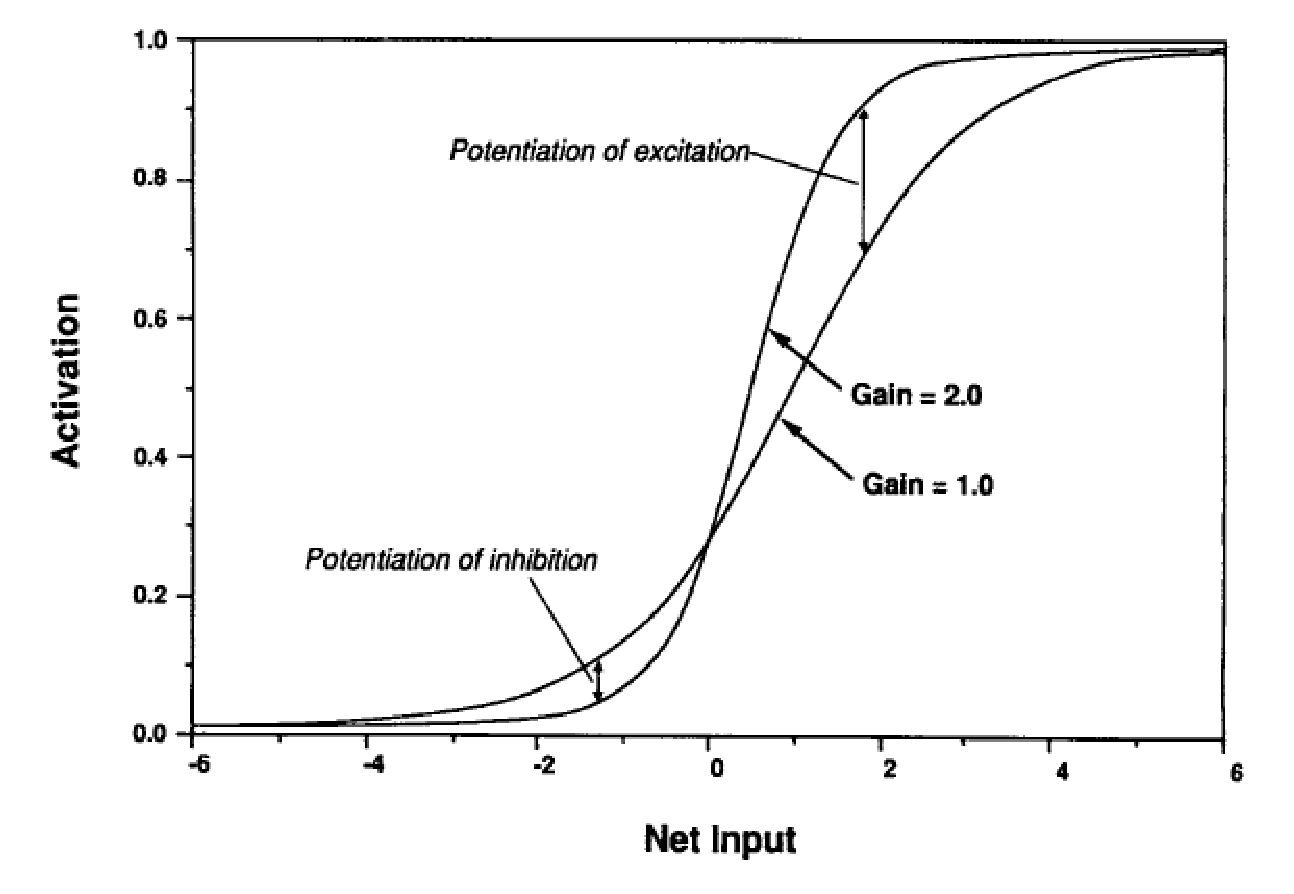
\includegraphics[width=100mm]{figures/gain_manipulation.eps}
\end{center}
\caption{Modeled effects of tonic DA on a standard activation function. An increase in the amount of DA heightens the effects of the net input, effectively increasing the signal-to-noise ratio in the network, while lower DA decreases the effects, reducing the signal-to-noise ratio. Image adapted from Cohen and Servan-Schreiber (1992).}
\label{gain-manipulation}
\end{figure} 

\subsubsection{Modeling Autism}
%In order to model the performance of people with autism, we propose to hinder the updating of the SRN context layer of the network as discussed previously.  Specifically, two distinct manipulations will be tested.  The first method will consist of gaussian noise being injected directly into the context layer of the SRN, resulting in contextual information which has been corrupted to varying degrees, based upon the amount of noise utilized.  In the second manipulation we will titrate the probability that the context layer is updated, mimicking a deficit flexible updating of the contents contained within the PFC.  This manipulation of the model is consistent with my proposed theory of impaired input and output gating of representations maintained within the PFC driven by DA interactions.  Importantly, this deficit will be instantiated from the beginning of development.  This is different than the modeled deficit proposed in Schizophrenia by Cohen and Servan-Schreiber, where the DA manipulation occurs after the task has been learned.   By instantiating a deficit in the context layer, the model may not be able to rely on temporally distant information, and, instead, must use the statistical regularities that are available at each time step.  The result should create a response bias towards the more frequently experienced words and a general inability to utilize context, as is observed in people with autism.

In order to model the performance of people with autism, we restricted the probability of successfully updating the Context Layer (PFC) upon each input presentation.  Specifically, we investigated successful PFC update probabilities of 100\% (control), 90\% and 80\%.  Preventing the updating of the PFC in this manner causes the temporally extended information normally contained within this layer to be much less reliable, making the learning of the sentential context difficult for the model to accomplish.  Without a reliable contextual representation of the previously presented information, the model will be forced to rely heavily the statistical frequency of the input corpus in order to learn the task.  Importantly, autism is believed to be a developmental disorder, with key neural differences likely present from very early on or even since birth.  To capture this fact, we restricted the ability of the modeled PFC layer to update throughout the entirety of training, simulating the deficit existing throughout key developmental periods.

\subsection{Lexical Dysambiguation Simulation Results}

\subsubsection{Overview}
Network simulations were repeated 10 times in each of the experimental conditions, with initial synaptic weights randomized for each repetition.  Each network experienced the entire training corpus 20 times.  The training corpus contains every potential context word / ambiguous homograph word pair, for a total of 200 different ``mini-clauses'', 100 with the contextual word presented first and 100 with the homograph occurring first in the clause.  Each of the ``mini-clauses'' are presented in a random order during each of the 20 blocks of training.  Lateral inhibition within the Output layer of network strongly encouraged the network to respond with a single ``word''.  The unit with the highest overall activation level was used as the model's response.  The key error measure across all conditions is the number of errors committed when assigning meaning to the ambiguous probe word and is visually presented in Figures~\ref{Schiz-Amb-Results} and \ref{ASD-Amb-Results}. The higher this measure, the worse the models performed on the disambiguation task.  

\subsubsection{Schizophrenia Model Results}
The model of homonym reading in schizophrenia was able to qualitatively match the behavioral data and reproduce the seminal modeling results of Cohen \& Servan-Schreiber (1992). (See Figure~\ref{Schiz-Amb-Results}.)  The ``Control'' network performed well regardless of the frequency of the meaning word (``Rare'' vs.``Common'').   Also, the ordering of contextual information had virtually no effect on model performance.  The model performed well regardless of if the context was presented early in the mini-clause (Context-First) or if it came later (Ambiguous-First).  However, as the PFC representations were systematically destabilized the error rate rose significantly. Importantly, this decrease in task performance only occurred when the context was presented first, but not when the context was presented last.  (See Figure~\ref{Schiz-Amb-Results}.)  
%Two-way ANOVAs were performed separately on each destabilization level -- 0\% Destabilized (Control), 33\% Destabilized, 66\% Destabilized, and 100\% Destabilized --, with frequency (``Rare'' vs. ``Common'') and ordering (``Context First'' vs. ``Meaning First'') as factors.  An effect of frequency was observed as the PFC was destabilized 33\%, 66\%, and 100\% (respectively, F(1,36) = 18.29, p $< .05$; F(1,36) = 57.48, p $< .05$; F(1,36) = 78.98, p $< .05$).  Also, an effect of ordering was observed for each condition (respectively, F(1,36) = 14.97, p $< .05$; F(1,36) = 77.72, p $< .05$; F(1,36) = 109.42, p $< .05$). Importantly, a there was a significant frequency by ordering interaction effect in all cases where the PFC was destabilized (respectively, F(1,36) = 11.99, p $< .05$; F(1,36) = 54.84, p $< .05$; F(1,36) = 73.49 p $< .05$).  This supports the observation that only the context first error rate rose significantly as a result of PFC destabilization. No effects were found in the control network results for either frequency F(1,36) = .64, p $>.05$; or ordering F(1,36) = 3.47, p $>.05$, and the frequency by ordering interaction was also non-significant F(1,36) = 1.77, p $>.05$.  This matches patterns of behavior reported in previous schizophrenia research~\cite{CohenJD:1992:Schizophrenia}, which demonstrated that people with schizophrenia have difficulty utilizing context when it is presented temporally distal from the homograph it is intended to disambiguate.    
%Two-way ANOVAs were performed separately on each destabilization level -- 0\% Destabilized (Control), 33\% Destabilized, 66\% Destabilized, and 100\% Destabilized --, with frequency (``Rare'' vs. ``Common'') and ordering (``Context First'' vs. ``Meaning First'') as factors.  An effect of frequency was observed as the PFC was destabilized 33\%, 66\%, and 100\% (respectively, F(1,36) = 18.29, p $< .05$; F(1,36) = 57.48, p $< .05$; F(1,36) = 78.98, p $< .05$).  Also, an effect of ordering was observed for each condition (respectively, F(1,36) = 14.97, p $< .05$; F(1,36) = 77.72, p $< .05$; F(1,36) = 109.42, p $< .05$). Importantly, a there was a significant frequency by ordering interaction effect in all cases where the PFC was destabilized (respectively, F(1,36) = 11.99, p $< .05$; F(1,36) = 54.84, p $< .05$; F(1,36) = 73.49 p $< .05$).  This supports my observation that only the context first error rate rose significantly as a result of PFC destabilization. No effects were found in the control network results for either frequency F(1,36) = .64, p $>.05$; or ordering F(1,36) = 3.47, p $>.05$, and the frequency by ordering interaction was also non-significant F(1,36) = 1.77, p $>.05$.  This matches patterns of behavior reported in previous schizophrenia research~\cite{CohenJD:1992:Schizophrenia}, which demonstrated that people with schizophrenia have difficulty utilizing context when it is presented temporally distal from the homograph it is intended to disambiguate.    

\subsubsection{Autism Model Results}
By restricting the ability of the Context Layer to update in a flexible manner, we was able to capture patterns of behavior consistent with previous findings of lexical disambiguation research in people with ASD~\cite{RefWorks:103,HappeF:1997:WCC_Homographs}. (See Figure~\ref{ASD-Amb-Results}.) Specifically, as the probability of updating the content of the modeled PFC layer was systematically reduced, the network became increasingly more reliant on the statistical frequency of the words.  Behaviorally this was manifested in a significantly higher error rate when the model needed to utilize contextual information, \emph{regardless of the temporal distance from the required response}, in order to correctly interpret the ``Rare'' meaning of the homograph in the sentence.  These results suggest that the model of autistic performance has difficulty utilizing contextual information to overcome a more frequent interpretation of a homograph, regardless of when it is presented in the sentence.  (See Figure~\ref{asd-lexamb-study}.) 
%Two-way ANOVAs were performed separately on each level of PFC updating  -- 100\% probability to update PFC (Control), 90\% probability to update PFC, and 80\% probability to update PFC -- with frequency (``Rare'' vs. ``Common'') and ordering (``Context First'' vs. ``Meaning First'') as factors.  An effect of frequency was observed in the ``autistic-like'' condition, where the PFC is restricted to update only 90\% and 80\% of the time (respectively, F(1,36) = 64.52, p $< .05$; F(1,36)=116.58, p $< .05$). However, an effect of ordering was not observed (respectively, F(1,36) = 0.35, p $> .05$; F(1,36) = 0.31, p $> .05$). Also, the frequency by ordering interaction was not significant in either case (respectively, F(1,36) = 0.87, p $. .05$; F(1,36) = 0.31, p $> .05$). These results suggest that the model of autistic performance has difficulty utilizing contextual information to overcome a more frequent interpretation of a homograph, regardless of when it is presented in the sentence.  No effects were found in the control network results for either frequency F(1,36) = .64, p $>.05$; or ordering F(1,36) = 3.47, p $>.05$, and the frequency by ordering interaction was also non-significant F(1,36) = 1.77, p $>.05$.  It is important to note that as the probability of updating the Context Layer was reduced, the model of autistic behavior performed worse overall when compared to the control network, including common interpretations of the homographs.   This pattern was not reported in the behavioral study of people with ASD.  However, the extremely low number of sentences in each condition (5) may be resulting in ceiling effects, limiting the ability to reliably detect this difference in their sample. (See Figure~\ref{asd-lexamb-study}.) 

%\& Servan-Schreiber (1992). See Figures~\ref{Schiz-Amb-First} \& \ref{Schiz-Context-First}.)  The ``Control'' network performed well regardless of the frequency of the meaning word (``Rare'' vs.``Common'') as well as if the contextual information came early in the mini-clause(Context-First) or if it came later (Ambiguous-First).  However, as the PFC representations were systematically destabilized (as is hypothesized to occur in schizophrenia due to tonic-DA dysfunction), the error rate rose significantly for when the context was presented first, but not when the context was presented last.  This matches patterns of behavior reported in previous schizophrenia research~\cite{CohenJD:1992:Schizophrenia}
%Also, the model added to the original modeling effort by allowing the contextual representations in the modeled PFC be learned from experience, instead of being hand-coded by the modeler.



\begin{figure}[tp]
\begin{center}
	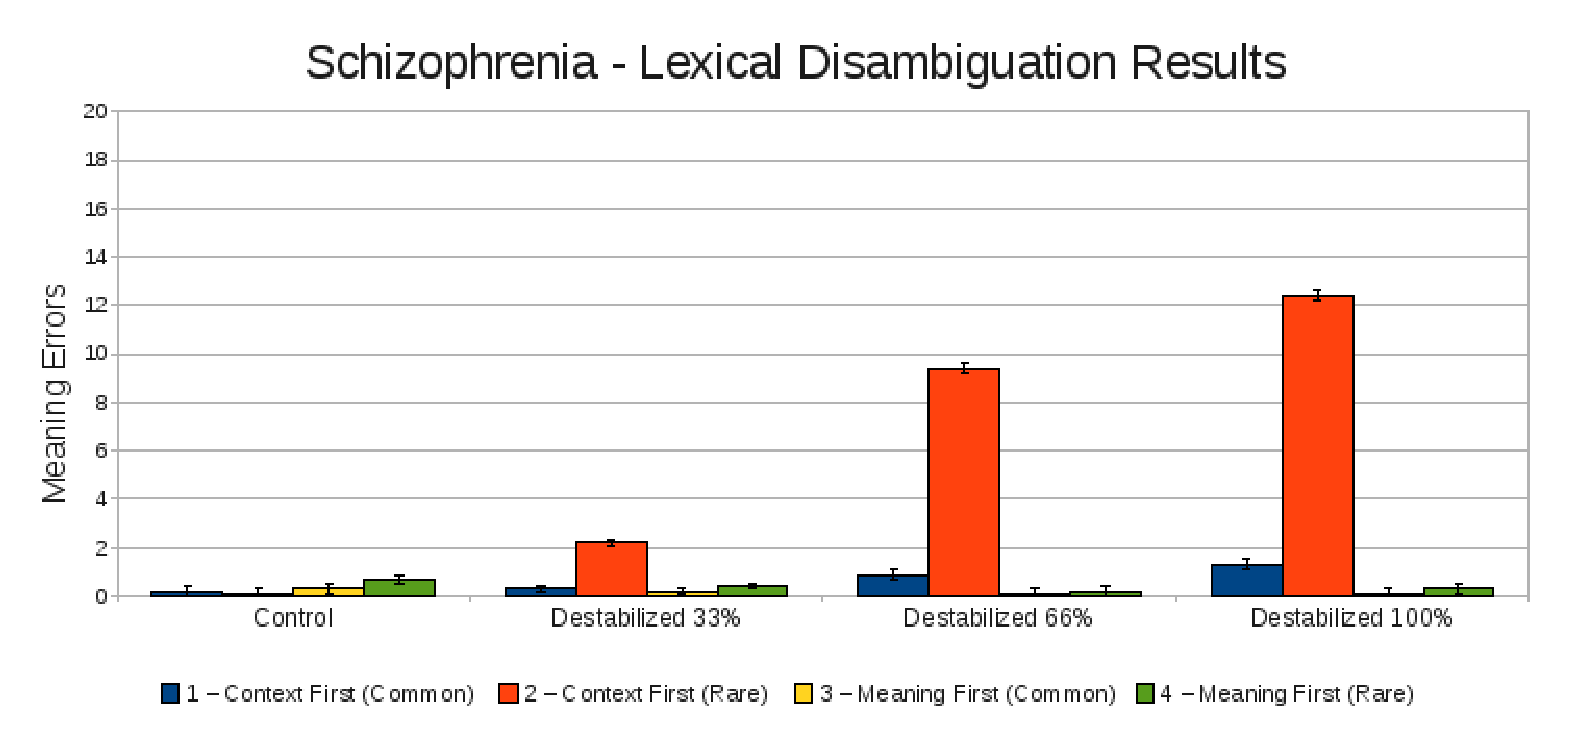
\includegraphics[width=140mm]{graphs/schiz_lexamb_results.eps}
\end{center}
\caption{Schizophrenia Model Results. As the modeled PFC is destabilized, the model performs selectively worse on condition (2).  In this condition the contextual information is presented first and the model must use this information to override the more common interpretation of the homograph. } 
\label{Schiz-Amb-Results}
\end{figure} 

\begin{figure}[tp]
\begin{center}
	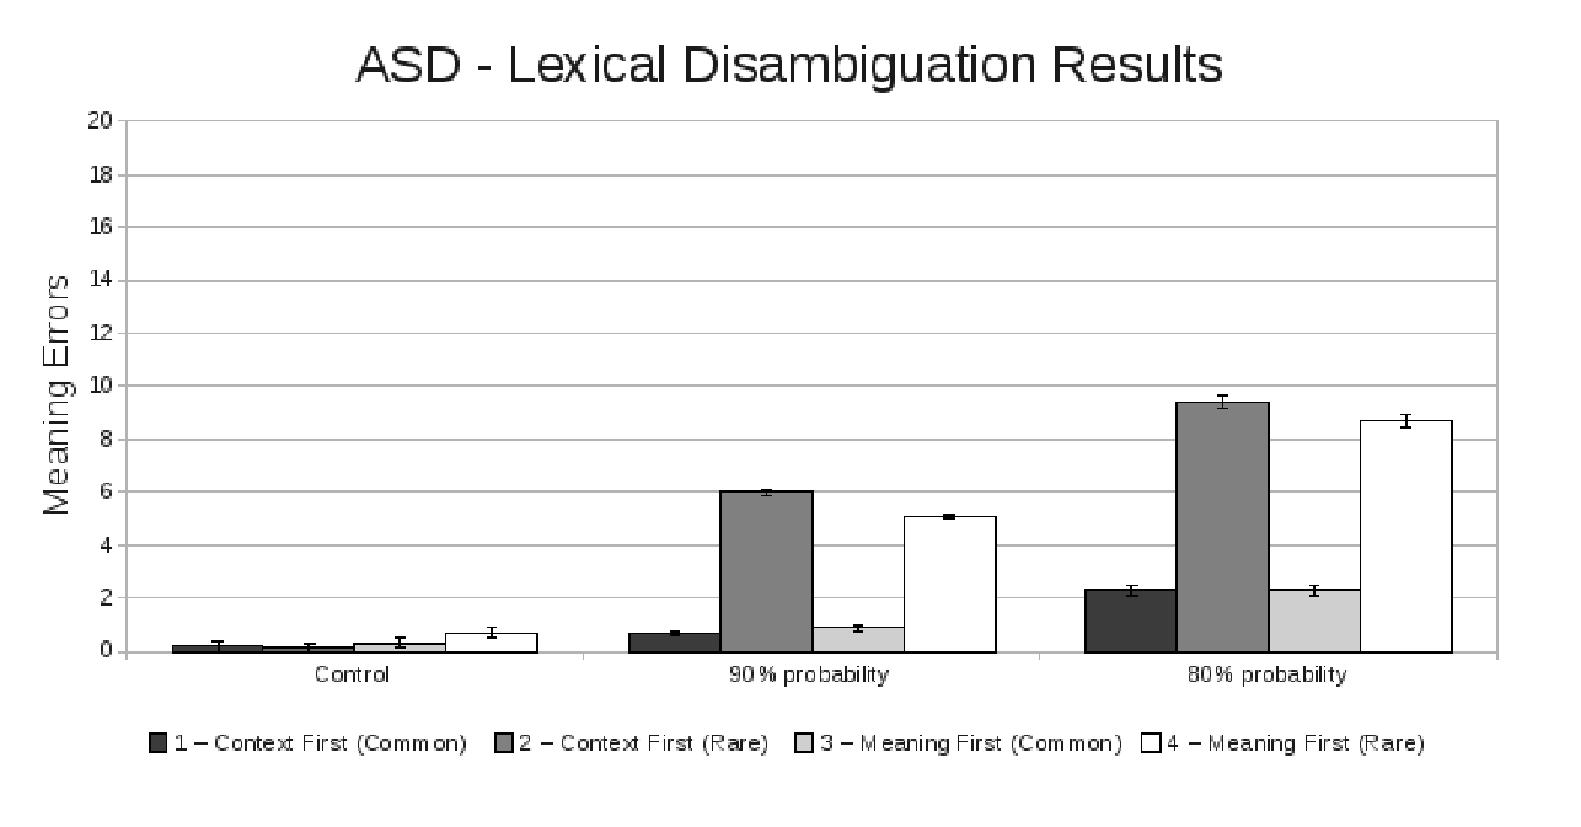
\includegraphics[width=140mm]{graphs/asd_lexamb_results.eps}
\end{center}
\caption{ASD Model Results. Systematically reducing the ability of the modeled PFC to update its contents resulted in worse performance on conditions (2) and (4).  These are the conditions that require the use of contextual information in order to override the more common interpretation of the homograph. } 
\label{ASD-Amb-Results}
\end{figure} 

%\subsection{Summary}
%In this chapter modeling results were presented demonstrating how a specific neural difference, dysfunctional interactions between the mid-bran DA system and PFC, can capture patterns of dysfunction in people with autism when utilizing sentential context to disambiguate the meaning of homographs.  Our work suggests that improper DA / PFC interactions lead to problems flexibly updating the contents of the PFC, and difficulties arise due to the lack of reliable contextual representations.  This causes the model to rely more heavily on statistical regularities in the environment.  In other words, the model adopts a policy of responding with the most common interpretation of a homograph in order to minimize errors, in lieu of appropriate contextual guidance from the Context Layer.  A previously published and theoretically justified computational model of lexical disambiguation was modified in a manner consistent with my hypothesis in order to capture the behavior of people with autism~\cite{CohenJD:1992:Schizophrenia}.  Interestingly, the Cohen \& Servan-Schreiber model was originally developed as an investigation into lexical disambiguation difficulties in people with Schizophrenia.  This provided my investigation with an interesting clinical comparison group, especially considering the qualitatively different behavioral profiles of the two disorders coupled with the suggestion of DA dysfunction underlying each respective pattern.  By positing the disorders actually have different \emph{kinds of DA dysfunction}, namely tonic DA dysfunction in schizophrenia and phasic DA abnormalities in ASD, the model is capable of explaining both the original findings of Cohen \& Servan-Schreiber and the patterns of behavior found in people with ASD~\cite{RefWorks:103,HappeF:1997:WCC_Homographs}.  




\section{Prototype Formation}
\label{section:prototype}

%
% Prototype Formation
%

\subsection{Category Learning in Autism}
Prototype formation is invaluable for learning concepts and categories. A category prototype is a kind of representational average of the features of category members that have been seen. Some studies have suggested that, when learning a new concept or category, children with autism are less likely to form a prototype representation than typically developing children~\cite{KlingerLG:2001:Prototype,GastgebHZ:2009:Prototype}. Difficulty identifying an abstract prototype is argued to underly the generalization problems found in ASD.

Typically developing children exhibit a ``prototype effect'' when they are shown objects in a category and are then asked to categorize novel objects. This effect involves more reliably and/or more quickly identifying a prototype object as a member of a target category, in comparison to other test objects. Klinger \& Dawson~(2001) \nocite{KlingerLG:2001:Prototype} found that people with ASD do not exhibit the ``prototype effect''.

In the Klinger and Dawson (2001) experiment, paricipants viewed cartoon pictures of imaginary animals, with each animal belonging to one of a small set of fictional animal categories. The members of each category of animal varied in four features. For example, animals in the ``Mip'' category varied in the sizes of horns, wings, mouths, and feet. Each feature could take on one of five discrete values, ordered 1 to 5 (e.g., horns always were of one of five specific sizes). Thus, individual cartoons could be specified by four feature values (e.g., ``5115'' for largest horns, smallest wings, smallest mouth, and largest feet). Different animal categories had distinct sets of four features, as illustrated in Figure~\ref{prototype-categories}.

The children initially learned to classify a target category of animals (e.g., ``Mip'') in contrast to a single non-target category (e.g., ``Pev''). A member of the target category was first dislayed, and the target category name was provided (e.g., ``This is a Mip.''). Participants were then presented with a series of target and non-target stimuli, one at a time, and they were asked to identify the members of the target category. As is clear from Figure~\ref{prototype-categories}, this category learning task was easy, as different animal categories possessed different sets of features. Corrective feedback was provided after each response. During this learning process, the presented target category stimuli only used feature values 1, 2, 4, and 5, but never 3. (See Figure~\ref{mip-familiarization}.) Only a subset of the possible combinations of feature values appeared, but the average value used for each feature in the target category was 3, making the unobserved ``3333'' stimulus object the prototype for the category.

Immediately following this learning process, participants were tested for the ``prototype effect''. On each test trial, two animals from the target category were juxtaposed, and participants were asked to select one as the ``best'' category member (e.g., ``Which is the best Mip?''). The trials of interest involved pairing the prototype (``3333'') with either a previously viewed animal or one that was novel but was composed only of previously viewed feature values (e.g., ``1425''). Typically developing children chose the prototype at a rate significantly higher than chance ($79\%$). However, children with autism selected the prototype at a rate indistinguishable from chance ($54\%$).
% (See Figure~\ref{klinger_results}.)
Klinger and Dawson argued that these results demonstrated a lack of prototype formation in ASD.

\begin{figure}[ht]
\begin{center}
	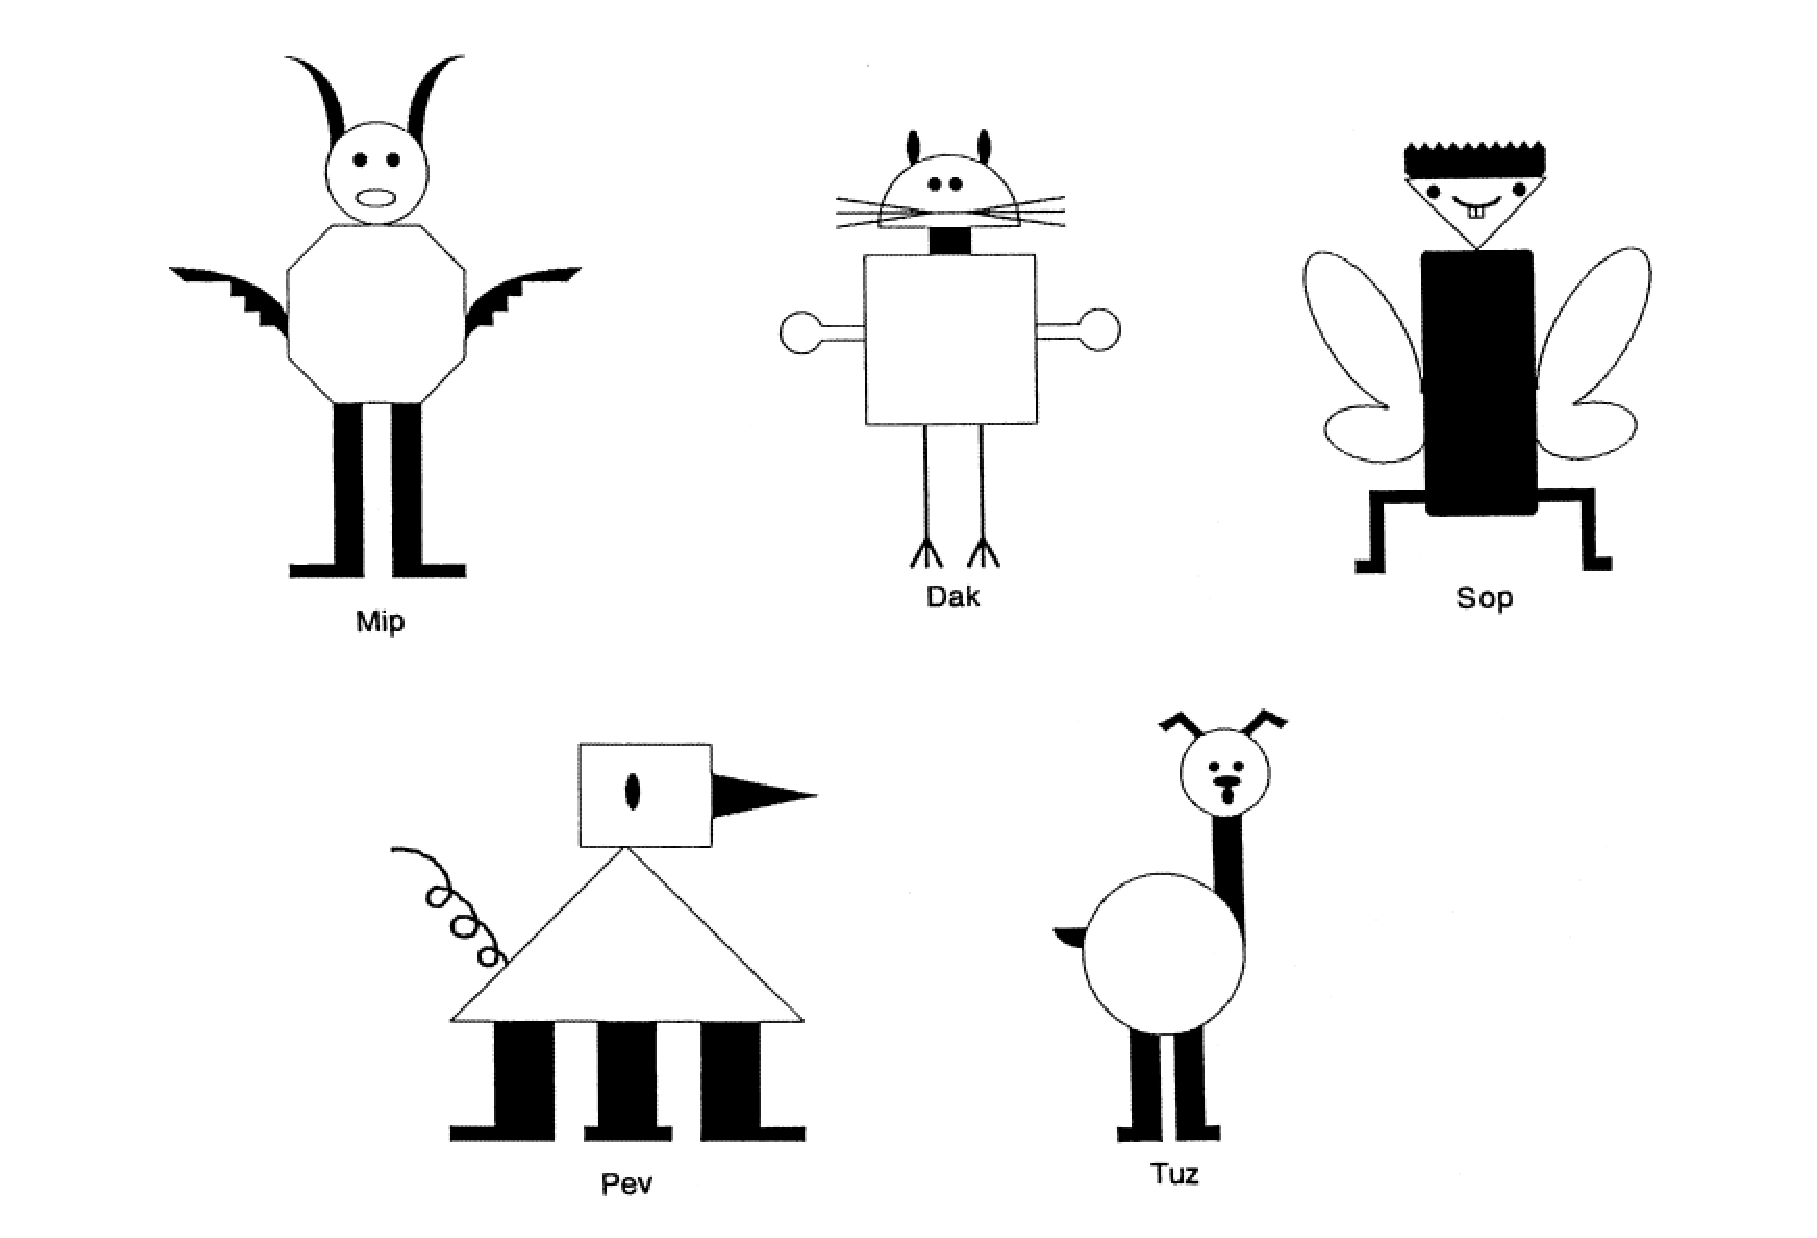
\includegraphics[width=160mm]{figures/prototype_categories.eps}
\end{center}
\caption{Prototypes for Different Stimulus Categories. Note that each participant observed members from only two categories. Image adapted from Klinger \& Dawson (2001).}
\label{prototype-categories}
\end{figure} 

\begin{figure}[ht]
\begin{center}
	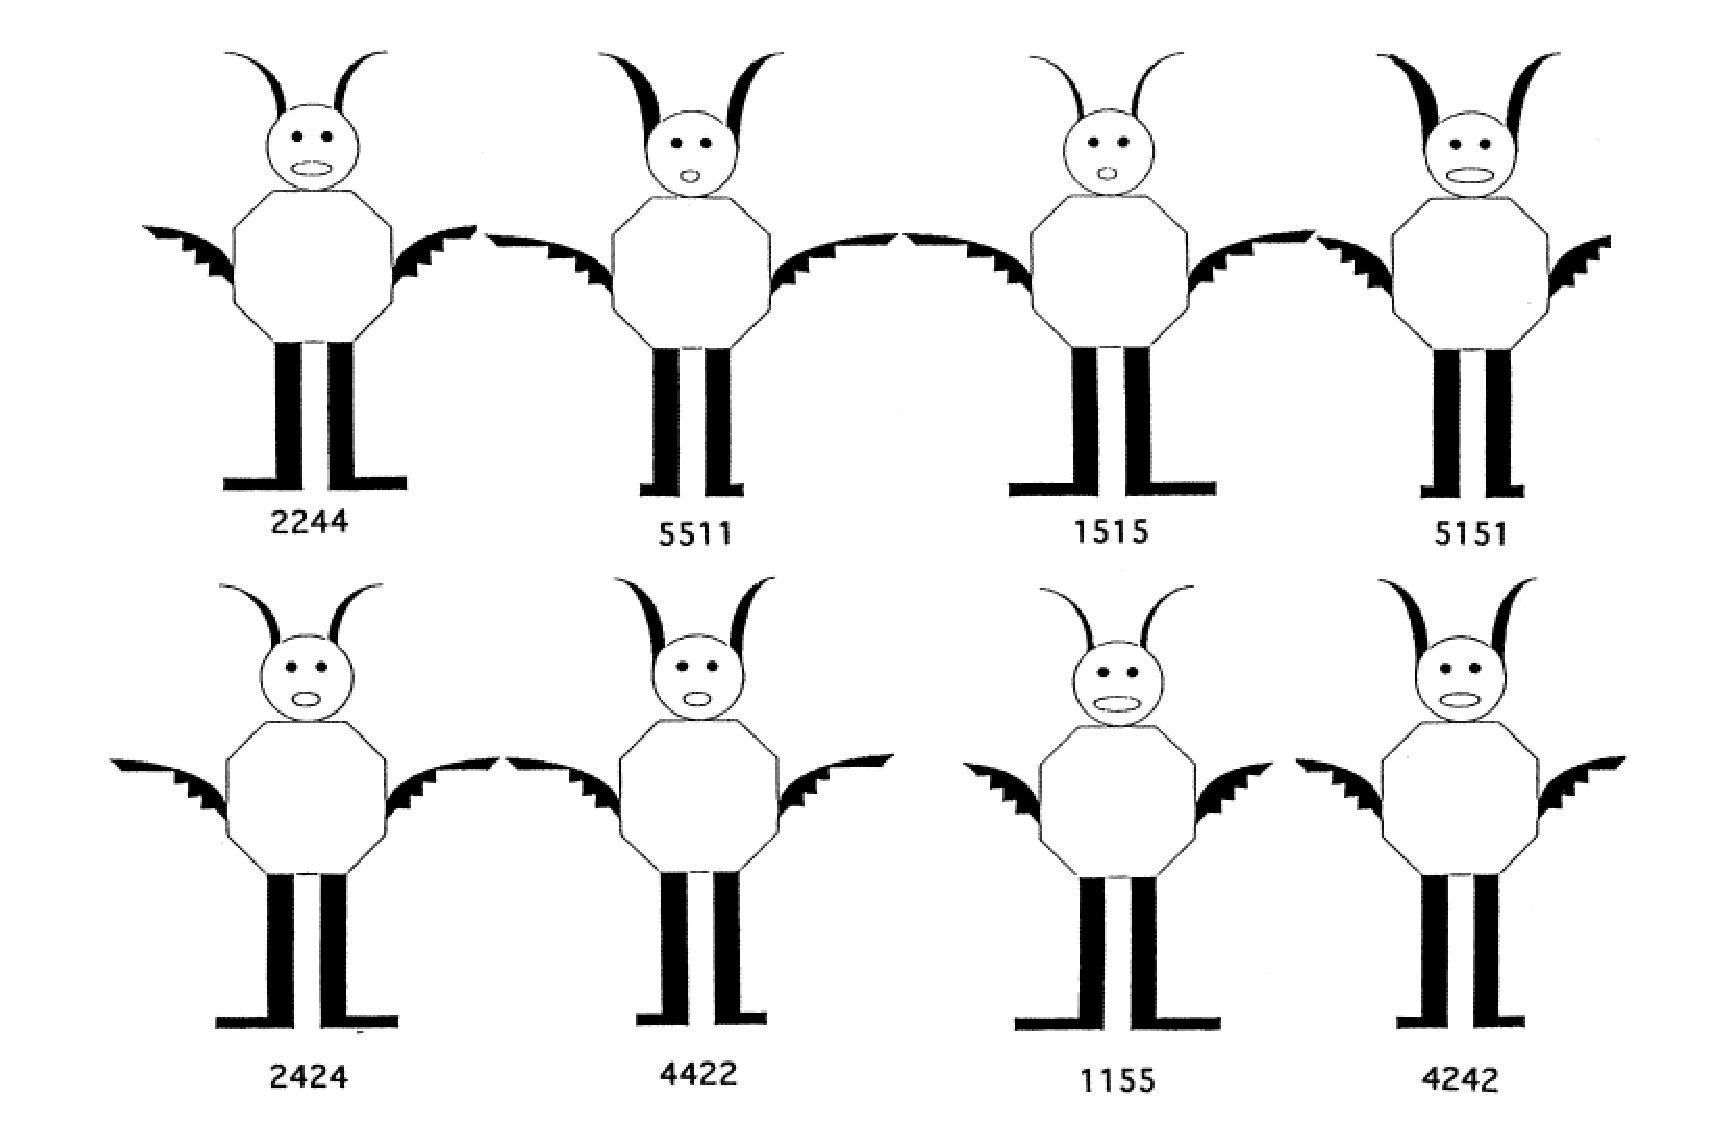
\includegraphics[width=160mm]{figures/mip_familiarization.eps}
\end{center}
\caption{Variation Within a Category. Image adapted from Klinger \& Dawson (2001).}
\label{mip-familiarization}
\end{figure} 

% DCN: WE NEED TO RECREATE THIS FIGURE WITH ONLY THE PROTOTYPE RESULTS!
% WE CAN ALSO LEAVE OUT THE DOWN SYNDROME BAR. THIS LEAVES SUCH A SIMPLE
% FIGURE THAT WE MIGHT WANT TO ELIDE THE GRAPH AND JUST REPORT THE 54 AND
% 79 PERCENT VALUES. INDEED, THAT IS WHAT I HAVE DONE.
% \begin{figure}[ht]
% \begin{center}
% 	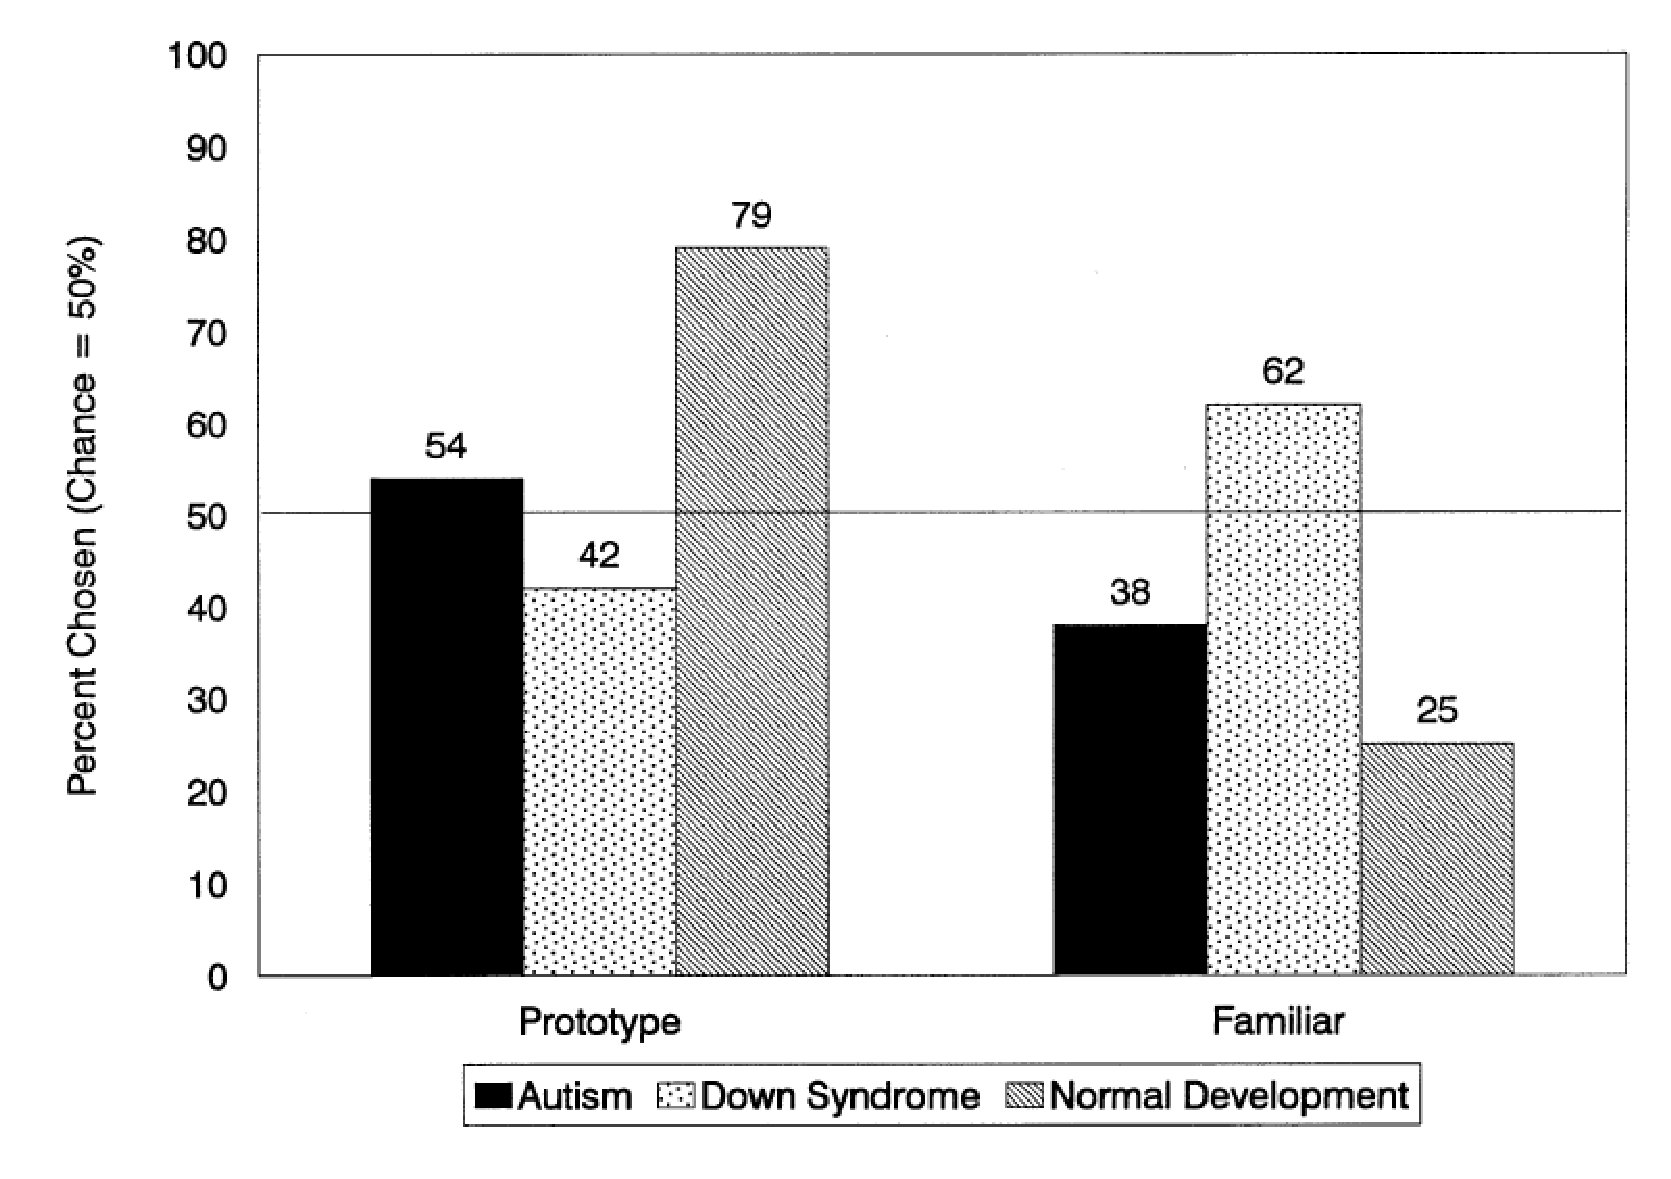
\includegraphics[width=110mm]{figures/klinger_results.eps}
% \end{center}
% \caption{Prototype Formation Results. The vertical axis shows the frequency with which the prototype was chosen over either a familiar or novel stimulus from the same category. Graph adapted from Klinger and Dawson (2001).}
% \label{klinger_results}
% \end{figure} 

\subsection{Modeling Category Learning with ALCOVE}
ALCOVE is a highly successful computational model of human performance on category learning tasks~\cite{KruschkeJK:1992:ALCOVE}. ALCOVE learns to categorize stimuli from corrective feedback on practice trials. There are three main processing layers in ALCOVE. An input layer represents the features of a current stimulus object. A hidden layer contains exponentially decaying radial basis function units, each of which becoming active to the degree that the current input is similar to that unit's preferred stimulus. The output layer contains one unit per category, with activation calculated as a weighted sum of hidden unit activity. The output activation levels are transformed into a probability distribution over category choices using a Luce choice ratio~\cite{LuceRD:1963:Ratio}. Learning arises from the adjustment of connection weights so as to reduce error~\cite{KruschkeJK:1992:ALCOVE}.

Importantly, ALCOVE also learns a set of attentional ``weights'' that reflect the relative importance of the various stimulus features for producing accurate categorization decisions. There is one weight value per stimulus feature (or ``dimension''), constrained to be between 0 and 1, with larger values indicating more sensitivity to variation in the given feature. ALCOVE's attentional weights determine the relative focus of the model on specific aspects of the stimulus, and are, therefore, analogous to the hypothesized role of PFC in directing top-down attentional control. (Consider the role of PFC in the previously described XT account of Stroop and WCST performance, focusing processing on specific aspects of the stimulus.) In the ALCOVE framework, PFC perseveration would involve restricting the attentional weights, limiting focus to one or a small number of the stimulus features.  

\begin{figure}[ht]
\begin{center}
	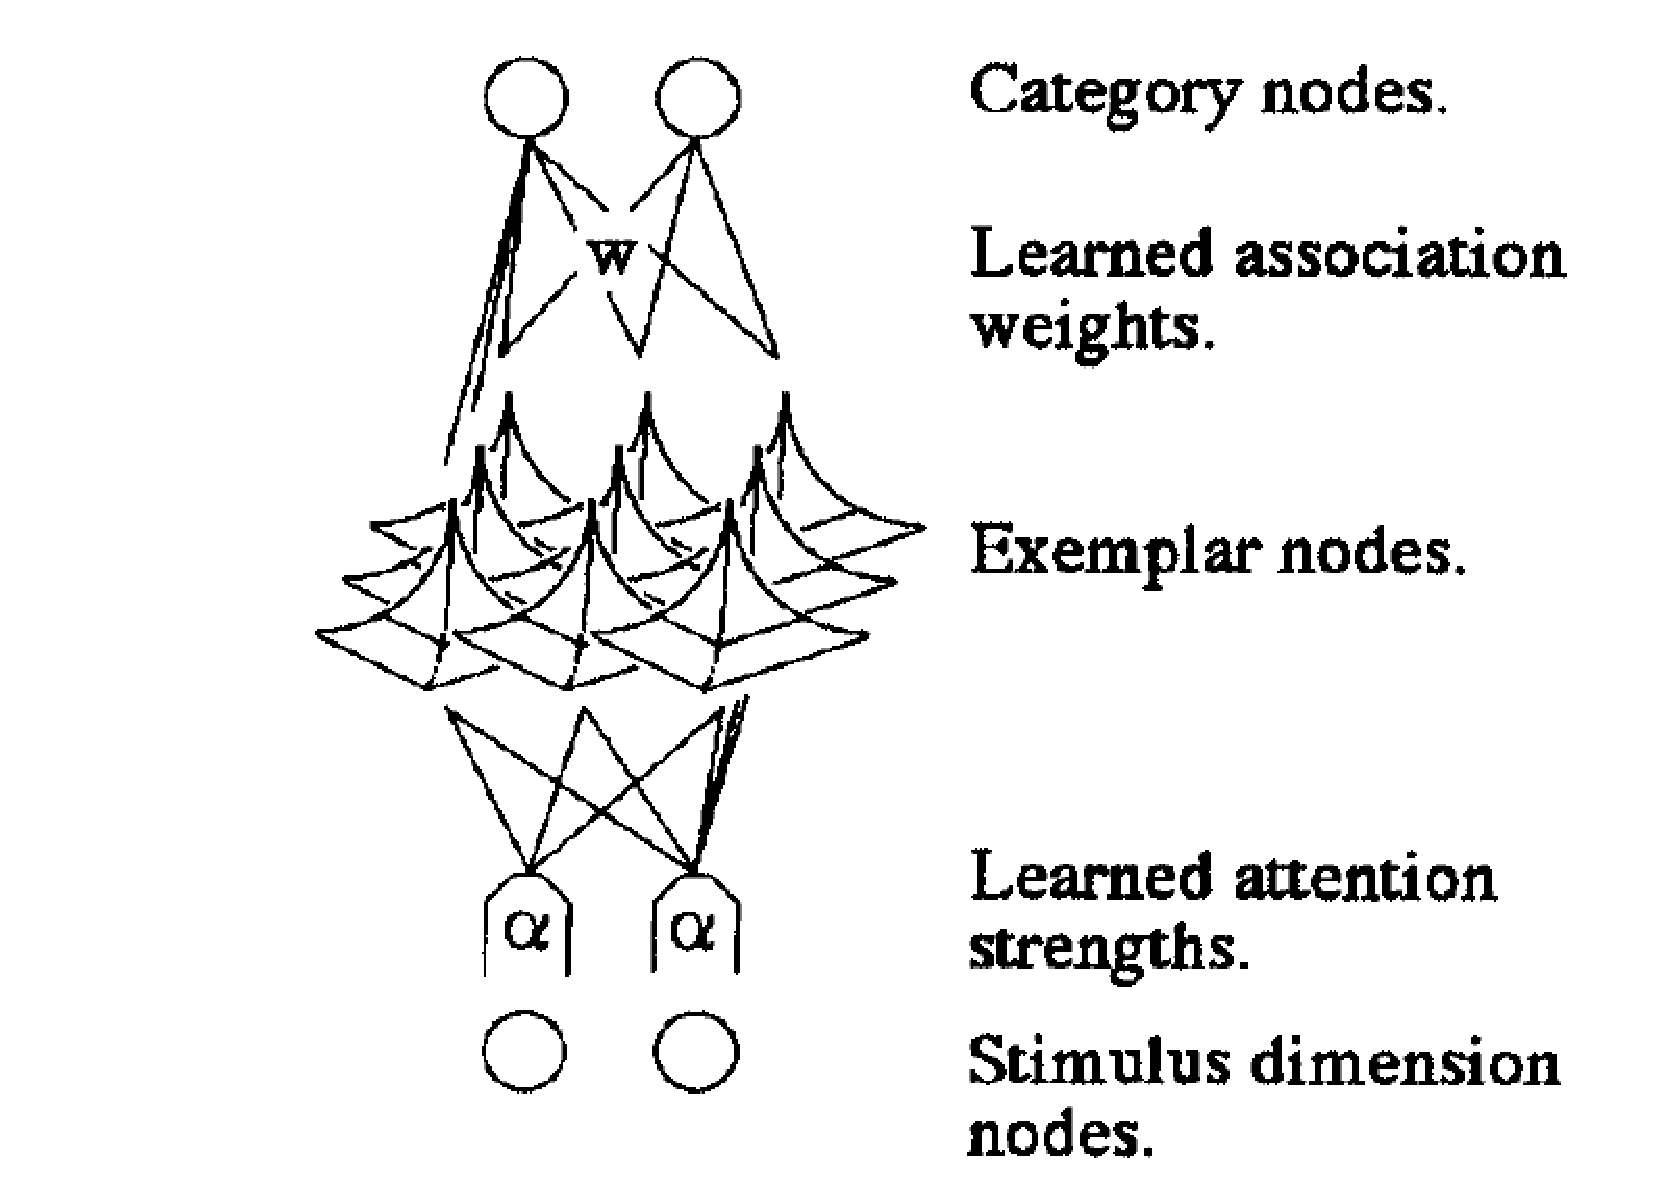
\includegraphics[width=100mm]{figures/alcove.eps}
\end{center}
\caption{Structure of ALCOVE (Attention Learning CoVEring map). Image adapted from Kruschke (1992).}
\label{alcove}
\end{figure} 

\subsection{Prototype Learning in ALCOVE}
We used ALCOVE to model the prototype formation study of Klinger \& Dawson (2001). Two output category units were used (e.g., ``Mip'' \& ``Non-Mip''). Four inputs, each with its own attentional weight, captured the four features that varied across members of the target category, with the 1--5 feature levels linearly scaled to 0.2--1.0 activations. (An activation of 0.0 was used to indicate the absence of a feature.) The model learned the target category from the same stimuli that were presented to children in Klinger \& Dawson (2001), with the standard ALCOVE error correction learning mechanism used to determine attentional and connection weights. Learning was disabled during subsequent testing for prototype formation.

% The training and testing of ALCOVE was modeled after the Klinger et al. study described above.  The training corpus was based on examples identical, in principal, to the target categories used during the familiarization trials. (See Figure~\ref{mip-familiarization}.)  As in the original study, eight familiarization trials were presented to the network during training.  On each presentation, the model labeled each target stimulus (e.g. this is a ``Mip'').  Only two response units, ``Mip'' \& ``Non-Mip'', were required.  Four input units, each with dimensional attention weights, were activated for each example presented to the network.  The four input units represent the four features used within each category in the study.  The level of activation for each input varied in a systematic fashion in accordance with the feature value of the stimulus.  For instance, if the stimuli presented has feature values (1551), the input vector presented to the network used the values (.20 1.0 1.0 .20). The standard ALCOVE error correction weight adjustments were used during the entirety of training.   After training ALCOVE on the familiarization stimuli, testing proceeded with all learning disabled in the model.  

Testing involved presenting the trained model with certain key stimulus objects and recording the activation of the target category output unit for each of them. The stimuli of interest included the prototype (``3333''), a stimulus seen during training (e.g., ``1515''), and a novel stimulus (e.g., ``1551''). For each pair of the prototype and another stimulus object, the recorded output activations were transformed into selection probabilities using a Luce choice ratio~\cite{LuceRD:1963:Ratio}. The mean probability of selecting the prototype over non-prototype stimuli was the measure compared to available experimental results.

% During testing, the prototype (3333) and the non-prototype test items, a novel stimuli (e.g. 1551) and a previously seen familiarization stimuli (e.g. 1515), were presented to ALCOVE separately.  The overall activation level of the output unit for the target category was recorded and used to determine which stimuli type was the ``preferred'' category example for ALCOVE. In order to compare model preference between prototype and non-prototype stimuli the activation levels were scaled to response probabilities using a Luce Choice Rule.   The average response probability for prototype versus non-prototype stimuli is the measure used in the comparison to the actual experiment results. 

\subsection{Modeling Autism in ALCOVE}
The ALCOVE model was modified in two ways to simulate neural differences in autism. First, we biased one randomly selected attentional weight to be high by initializing its value to $0.9$. The other attentional weights were initialized to $0.1$. This manipulation captures, at a gross level, our conjecture that deficient DA based gating of PFC results in overly perseverative control over top-down attention, effectively restricting the features used during processing. In the control version of the model, the attentional weights were all initialized to $0.1$, as is standard in ALCOVE. Attentional weights were adjusted during the category learning process, using the standard ALCOVE method for doing so. The second modification reflected the claim that ASD involves hyper-specific perception and behavior~\cite{HappeF:1999:WCC}. The ALCOVE ``specificity'' parameter, which controls the rate of exponential decay in the activation function of the hidden units, was increased from its standard value of $1.0$ to $2.5$ in the autism model. This caused each hidden unit in the autism model to become strongly active for a more restricted range of stimuli.

%One additional ALCOVE parameter was adjusted in order to better simulate the performance of people with autism on the categorization task.  The standard ALCOVE equation for the activation levels of the exponentially decaying hidden units contains a multiplicative scaling parameter referred to  by Kruschke as ``specificity''.  Increasing the specificity parameter makes the hidden units hyper-specific, sensitive to a more-restrictive range of features in the environment.  This is interesting because many researchers have argued that people with autism exhibit hyper-specific behavior in their everyday lives~~\cite{McClellandJL:2000:Autism,HappeF:1999:WCC}.  In the results described next, the specificity parameter in ALCOVE was adjusted from 1.0 in the control network to 2.5 for the network modeling behavior of people with ASD.  

%The simulated performance of people with autism will be contrasted with the control case, believed to capture normally developing people's performance on such tasks.  The performance of both autistic and control ALCOVE models will be directly compared to the data collected by Klinger and Dawson (2001). 

\subsection{Simulation Results}
Model simulations were repeated $80$ times in each experimental condition, with each repetition treated as an individual subject for data analysis. The control network exhibited the ``prototype effect'' observed in typically developing children, choosing the prototype over the non-prototype $70.52\%$ of the time.
% (See Figure~\ref{alcove-results}.)
For consistency, we used the same analysis as Klinger \& Dawson (2001), a one-sample T-test, in order to determine if the model's preference for the prototype was reliably different than chance (50\%). Analysis of the control model's performance indicated that the ``prototype effect'' was reliably larger than chance ($p < 0.0001$). The ASD model, however, preferred the prototype only $52.91\%$ of the time, which was not reliably different than chance ($p > 0.30$). This matches the lack of a ``prototype effect'' in people with autism reported in previous studies~\cite{KlingerLG:2001:Prototype,GastgebHZ:2009:Prototype}.

% DCN: Once again, it doesn't seem to make sense to have a figure for
% the display of only two values, given our space constraints.
% \begin{figure}[ht]
% \begin{center}
% 	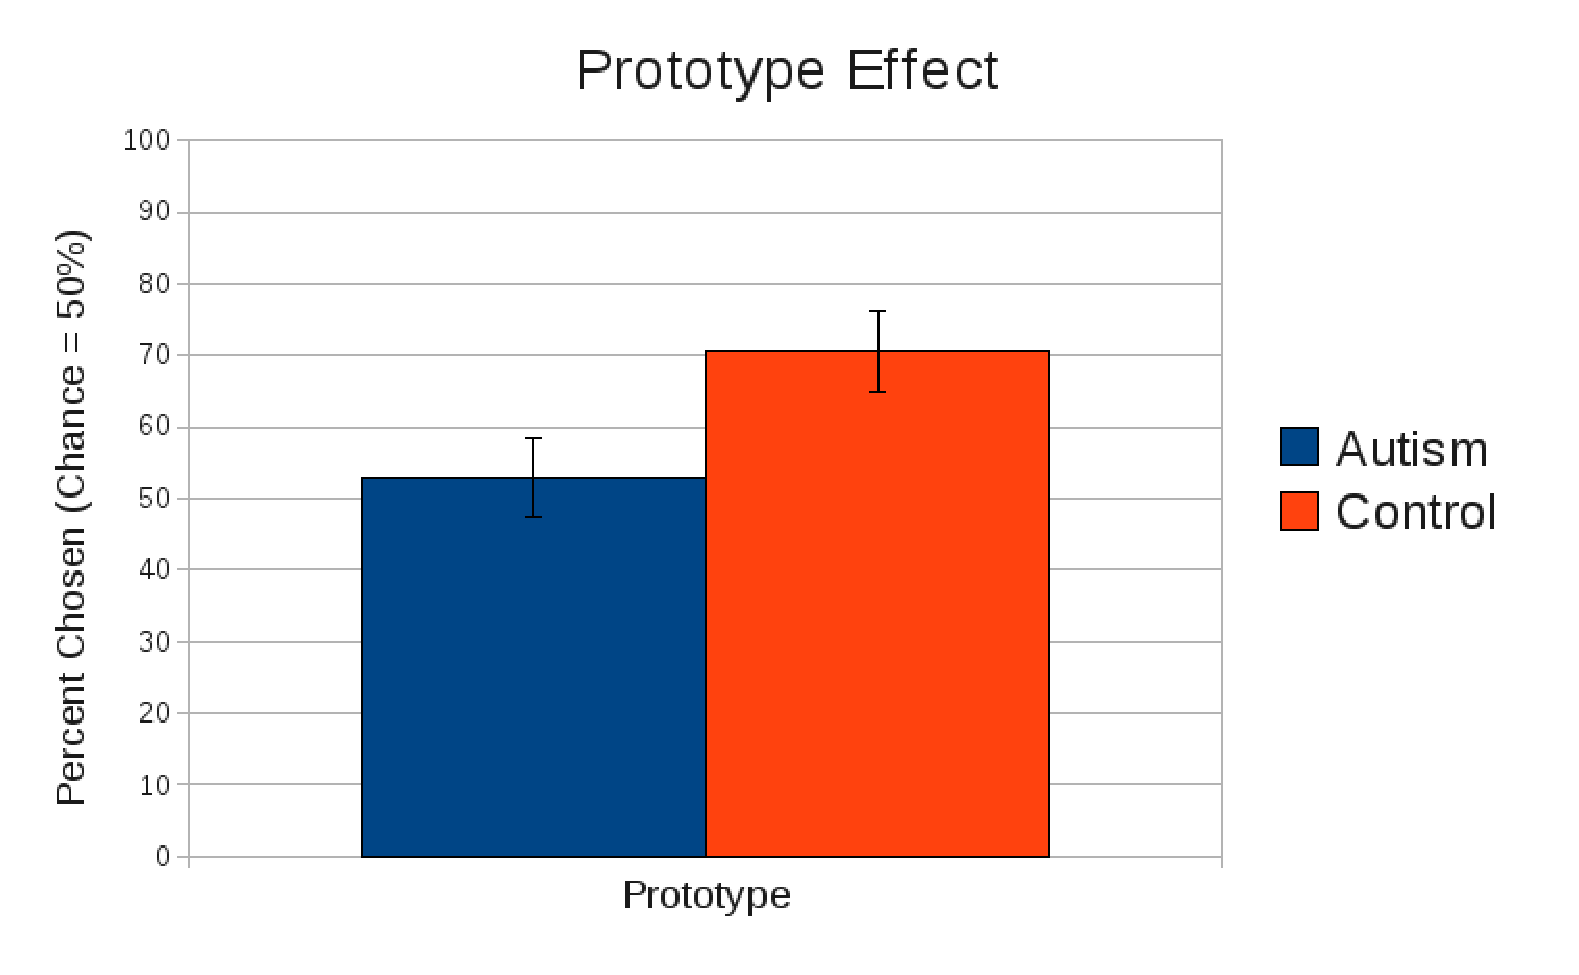
\includegraphics[width=100mm]{graphs/alcove_results.eps}
% \end{center}
% \caption{ALCOVE Model Results.  The measure on the y-axis is the percentage times that the prototypical animal was chosen by the model over the non-prototype choices.  In the control network, the prototype was chosen 70.52\% of the time on average, demonstrating a strong prototype effect and matching the human subject experiment results.  However, the model of autistic performance chose the prototype on average only 52.91\% of the time over the non-prototype stimuli.  Statistical analysis reveal that the control network chose the prototype at a rate significantly greater than chance ($p < .0001$) while the ASD network was not statistically distinguishable from chance ($p > .30$).}
% \label{alcove-results}
% \end{figure} 

\subsection{Summary}
These results show that failures at prototype formation in autism can be explained in terms of our hypothesized DA/PFC deficit. Restricting ALCOVE's attentional mechanism to hinder the flexible consideration of all stimulus features results in a lack of prototype preference. It is worth noting that matching the specificity parameter of the control model to match that of the autism model ($2.5$) does not change the presented pattern of results. This is evidence that it was the adjustment of initial attentional weights in the autism model, reflecting perseveration in PFC guided attention, that drove the observed difference.




\section{Future Directions}
\label{section:future}

%
% Future Work
%

\textbf{FILL ME IN, OR REMOVE THIS SECTION}




\section{The Utility of Computational Models for Understanding Autism}
\label{section:modeling}

%
% The Utility of Computational Models for Understanding Autism
%

\subsection{Computational Cognitive Neuroscience}
An important contribution of this work involves the fact that it uses a relatively novel tool in ASD research: the methods of computational cognitive neuroscience. These methods provide a way to formalize how differences in the underlying neural circuitry give rise to the patterns of behavior found in people with autism. Specifically, we modified previously published and validated computational models of human behavior in accordance with the hypothesis that autism involves dysfunctional PFC/DA interactions, hindering updating of PFC contents. These modified models were shown to capture the behavioral performance of people with autism. This approach allowed us to offer a unified biological explanation for autistic behavior in the diverse areas of executive dysfunction, an implicit learning task, lexical disambiguation, and category learning. Indeed, the strength of the work presented here is not in any single model, but in providing a unified, plausible, precise neural mechanism that is capable of providing a kind of intertheorhetic reduction previously absent in ASD research. This work provides an example of the important role that computational cognitive neuroscience can play in improving our understanding of autism and other developmental disorders.

\subsection{Previous Computational Models of Autism}
The formal and explicit nature of computational cognitive modeling offers a novel approach to autism research. In order for computational models to be useful in this endeavor, they must be constrained by both bottom-up (neurobiological mechanisms) and by top-down (observed behavior) considerations, providing a formal characterization of the relationship between these levels of analysis. While there have been some previous computational models of ASD, it is not at all clear that they have offered such an explicit and detailed connection between biology and behavior.

Some previous computational models have attempted to address specific behavioral aspects of autism, including poor generalization~\cite{CohenIL:1994:AutismLearning,GustafssonL:1997:AutismMaps}, Weak Central Coherence~\cite{OLoughlinC:2000:Coherence}, and overselectivity~\cite{McClellandJL:2000:Autism}. One ambitious computational framework, developed by Grossberg \& Seidman (2006)~\nocite{GrossbergS:2006:Autism}, offers an explanation of multiple aspects of autism, including poor generalization, as well as cognitive and emotional issues.

A shortcoming of many of the existing models of autism is their fairly abstract nature, making little contact with specific neurobiological properties or measures~\cite{CohenIL:1994:AutismLearning,McClellandJL:2000:Autism,OLoughlinC:2000:Coherence}. Models that have incorporated biology have, thus far, only matched qualitative patterns of behavior rather than attempting to account for any quantitative behavioral data~\cite{GustafssonL:1997:AutismMaps,GrossbergS:2006:Autism}. Models that are more tightly constrained by both neurobiological mechanisms and quantitative behavioral data, such as the models presented in this chapter, may have a more profound impact on our understanding of autism.



\section{Conclusion}
\label{section:conclusion}

%
% Conclusion
%

As awareness and resources continue to grow, so does the overall number of diagnoses of people with ASD.  At the same time, ASD continues to pose a massive challenge to researchers.  While great progress is being made in areas such as early identification of ASD, as well as intervention techniques, to date there is no sign of a converging consensus as to the true neural underpinnings of ASD.  Further complicating our understanding of the mechanisms that may underly autism is a staggeringly diverse behavioral profile as well as multiple physical abnormalities that often accompany a diagnosis.  In this document, we have presented a program of research in an attempt to address some of these issues.  Dopamine has diffuse and widespread effects of throughout the human cortex. This coupled with strong ties to multiple clinical populations as well as numerous ties to human behavior make it an intriguing initial candidate for a disorder possessing a profile like that of autism.  However, it is not until we recognize the myriad of ties between DA and core autistic behavioral differences that we begin to see the true potential of the DA dysfunction hypothesis of ASD.  Increased seizure rates, motor abnormalities, stereotyped and repetitive behaviors, executive dysfunction, abnormal gaits, problems learning to follow eye gaze, and attentional abnormalities are all key components of behavior in autism, and all are linked tightly to the mid-brain dopamine system~\cite{RefWorks:99,RefWorks:100,RefWorks:102,HillEL:2004:AutismExecutiveDysfunction,RefWorks:1,RefWorks:3,RefWorks:5,RefWorks:2,RefWorks:109}, supporting the argument for a role for the dopaminergic system in the etiology of autism. Importantly, we have argued that perturbed DA / PFC interactions may lead to overly perseverative attention in autism, providing a neurally precise and plausible mechanism that might link previously disjoint theories in autism research. 

By separating the mechanisms responsible for cognitive control and the flexible adjustment of control, perplexing aspects of the specific executive dysfunction profile demonstrated by people with autism are nicely captured.  Cognitive control is instantiated via actively maintained control representations within the prefrontal cortex.  Cognitive flexibility is implemented via interactions between PFC and the mid-brain dopamine system.  These interactions are suspect in autism, resulting in problems in flexibly updating the control instantiated via the PFC and capturing the problematic profile demonstrated by people with ASD~\cite{HillEL:2004:AutismExecutiveDysfunction}.  Developmentally, executive dysfunction does not appear until later in childhood.  My modeling efforts indicate that this may occur due to the protracted development of the PFC.  In our model, early performance is driven largely by non-frontal, more posterior, brain systems which are largely unaffected by the posited DA-related abnormalities in autism.  As the PFC becomes more effective, differences in PFC/DA interactions are unmasked.  

%Stimulus overselectivity, where a restricted subset of possible items or features in the environment dominate behavior in people with ASD, can also be subsumed under the same theoretical framework.  We hypothesize that frequent and flexible updating of the attentional and control representations stored in the PFC is necessary in order to prevent an overly restricted subset of items in the environment from gaining control over our behavior.  Under this account, inflexible and infrequent updating results in a restricted subset of features from the environment dominating the contents maintained within the PFC.  Subsequently, through an associative learning process, the restricted subset comes to possess stronger ``association weights'' and thus dominate responding compared to the other features in the environment.

In another area of interest, weak central coherence theorists posit that people with autism have difficulties integrating pieces of information into a coherent whole or ``gestalt''\cite{FrithU:1989:AutismWCC,HappeF:1999:WCC}.  A major contribution of this work is demonstrating how top-down PFC-like mechanisms may influence the representations learned in other cortical areas.  As such, WCC may be recast not as a problem in the integration of information per se, but rather as integrating the \emph{wrong} information, due to the inflexible updating of attentional / control representations stored within the PFC.   Problems with implicit learning as well as using contextual information to disambiguate sentential context can both be explained utilizing this account.  Tasks investigating implicit learning, such as the Serial Response Time Task (SRTT), depend on previous information about the sequence to be readily available on subsequent time steps in order for normal learning to occur.  Without reliable contextual information, neural systems will struggle to integrate the past information in an appropriate manner.  The same is true when determining the meaning of ambiguous words in a sentence, without an appropriate representation of the context, the best we can do is to rely on the statistical frequency of the words we experience.   

Finally, people with autism also demonstrate an atypical prototype effect when learning category structures~\cite{RefWorks:113,StraussMS:2009:Prototype}.   It is reasonable to assume that in order to correctly form and use a prototype, we must have the ability to spread our attention out somewhat evenly across the relevant features of a stimulus or category example.  If, as would be caused by inflexible attentional of the PFC, we highlight and learn to ``over-value'' a restricted subset of the features, the representation that is learned would likely not represent the standard mathematical average of psychological feature values as is argued to occur during prototype formation.  In this case, an individual may become ``overselective'' and weight the restricted subset of feature values more highly during category determination.  

The convergence of data supporting dopamine's role in autism, combined with the possibility of providing a conceptual bridge spanning multiple theories in autism, is extremely encouraging.  Computational modeling results presented in this document help to demonstrate the potential for formal computational models investigating the links between possible neural underpinnings and behavior in people with ASD.  Using simulations, constrained and informed by both biology and observed behavior, precise and testable predictions of underlying mechanisms can be made, providing a theoretical bridge between psychological and anatomic theories of ASD.   Namely, our modeling efforts suggest that dysfunctional interactions between the mid-brain DA system and the PFC may lead to overly perseverative top-down attentional effects in people with ASD.  By casting the PFC as key player in both attention and in the shaping of posterior cortical areas, our theory provides a way to unify multiple previously disparate behavioral phenomena observed in people with ASD.



\bibliography{ed,thesis_ref}

\end{document}

